% !TEX program = xelatex
\documentclass[12pt,a4paper,fontset=fandol]{ctexart}
\usepackage[left=22mm,right=22mm,top=22mm,bottom=22mm]{geometry}
\usepackage{amsmath,amssymb,bm,mathtools}
\usepackage{graphicx,xcolor,booktabs,longtable,array}
\usepackage{tikz}
\usetikzlibrary{arrows.meta,calc,decorations.pathmorphing}
\usepackage{setspace,enumitem,fancyhdr}
\usepackage[unicode,hidelinks]{hyperref}
\setstretch{1.24}
\setlength{\parindent}{2em}
\setlength{\parskip}{.35em}
\setlength{\emergencystretch}{2em}
\setlist{nosep,leftmargin=2em}
\setcounter{secnumdepth}{-1}
\ctexset{section={format=\Large\bfseries,beforeskip=1em,afterskip=.7em},
subsection={format=\large\bfseries,beforeskip=.8em,afterskip=.4em},
subsubsection={format=\normalsize\bfseries,beforeskip=.7em,afterskip=.3em}}
\allowdisplaybreaks[2]
\tikzset{arr/.style={-{Stealth[length=2mm]},semithick},
dot/.style={circle,fill,inner sep=1.5pt}}
\providecommand{\tightlist}{\setlength{\itemsep}{0pt}\setlength{\parskip}{0pt}}
\providecommand{\pandocbounded}[1]{#1}
\newsavebox{\diagrambox}
\pagestyle{fancy}
\fancyhf{}
\renewcommand{\headrulewidth}{0pt}
\fancyfoot[C]{\small \thepage}
\setlength{\headheight}{16pt}
\begin{document}
\begin{titlepage}
\thispagestyle{empty}
\vspace*{27mm}
\begin{center}
{\LARGE\bfseries 第43届全国中学生物理竞赛\par}
\vspace{8mm}
{\LARGE\bfseries 复赛理论试题\par}
\vspace{17mm}
{\Large 教师备课版\par}
\end{center}
\vfill
\end{titlepage}
\setcounter{page}{1}
\section{第 1
题　非线性正四面体电阻网络}\label{ux7b2c-1-ux9898-ux975eux7ebfux6027ux6b63ux56dbux9762ux4f53ux7535ux963bux7f51ux7edc}

如图1-1，六个非线性电阻连成正四面体网络，顶点为
\(A,B,C,D\)，导线电阻忽略不计。连接 \(i,j\) 两顶点的电阻满足
\(I=c_{ij}V^3\)，其中 \(V\) 为沿电流方向的电压降，\(c_{ij}>0\)。已知

\[
c_{AB}=\frac{\kappa}{9},\quad c_{AC}=c_{DB}=16\kappa,\quad
c_{AD}=c_{CB}=\kappa,\quad c_{CD}=8\kappa.
\]

在 \(A,B\) 两点间施加恒定电压 \(V_0>0\)，总电流由 \(A\) 流入、由 \(B\)
流出。求总电流 \(I_{\text{总}}\) 和端口等效电阻
\(R_{\rm eq}\)。本题45分。

\begin{center}
\begin{minipage}{\linewidth}
\centering\begingroup
\sbox{\diagrambox}{\small
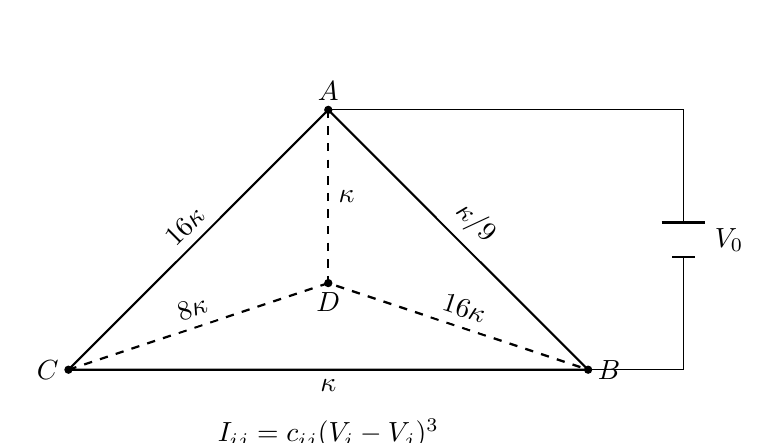
\begin{tikzpicture}[x=1.1cm,y=1.1cm]
\coordinate (A) at (0,3); \coordinate (B) at (3,0);
\coordinate (C) at (-3,0); \coordinate (D) at (0,1);
\draw[thick] (A)--node[fill=white,sloped,above] {$16\kappa$}(C)
 --node[fill=white,below] {$\kappa$}(B)
 --node[fill=white,sloped,above] {$\kappa/9$}(A);
\draw[thick,dashed] (A)--node[fill=white,right] {$\kappa$}(D);
\draw[thick,dashed] (C)--node[fill=white,sloped,above] {$8\kappa$}(D)
 --node[fill=white,sloped,above] {$16\kappa$}(B);
\foreach \p/\pos in {A/above,B/right,C/left,D/below}
 {\fill (\p) circle (1.5pt); \node[\pos] at (\p) {$\p$};}
\draw (A)--(4.1,3)--(4.1,1.7);
\draw (B)--(4.1,0)--(4.1,1.3);
\draw[thick] (3.85,1.7)--(4.35,1.7);
\draw[thick] (3.97,1.3)--(4.23,1.3);
\node[right] at (4.35,1.5) {$V_0$};
\node at (0,-.75) {$I_{ij}=c_{ij}(V_i-V_j)^3$};
\end{tikzpicture}
}
\ifdim\wd\diagrambox>.88\linewidth
\sbox{\diagrambox}{\resizebox{.88\linewidth}{!}{\usebox{\diagrambox}}}
\fi
\ifdim\ht\diagrambox>.29\textheight
\resizebox{!}{.29\textheight}{\usebox{\diagrambox}}
\else\usebox{\diagrambox}\fi
\par\smallskip{\small 图1-1　正四面体的六条支路及其非线性系数；线段在投影中的交叉处不连接。\par}
\endgroup\end{minipage}
\end{center}

\subsection{一、题型定位}\label{ux4e00ux9898ux578bux5b9aux4f4d}

这是非线性电阻网络的节点电势问题。各支路的电流由电压降的三次方决定，不能先把它们换成一组固定电阻，再直接使用普通电桥的串并联计算。

解题的第一层任务是求内部节点 \(C,D\) 的电势。第二层任务是把由端口 \(A\)
流出的三条支路电流相加。网络存在交换
\(A\leftrightarrow B\)、\(C\leftrightarrow D\)
的结构对称性，但这种对称性给出的是 \(V_C+V_D=V_0\)，并不表示
\(V_C=V_D\)。

\subsection{二、知识点}\label{ux4e8cux77e5ux8bc6ux70b9}

\begin{itemize}
\tightlist
\item
  稳恒电流满足节点电流守恒，非线性伏安关系不改变基尔霍夫定律。
\item
  采用有向电压时，可统一写
  \(I_{ij}=c_{ij}(V_i-V_j)^3\)，负值表示实际电流反向。
\item
  电势参考点可以任取，物理量只依赖电势差。
\item
  严格单调函数取值相等时，自变量相等。
\item
  端口比值电阻 \(V_0/I_{\text{总}}\) 与微分电阻 \(dV_0/dI_{\text{总}}\)
  是不同的量。
\item
  同一端口条件下，所有支路均单调耗散的连通网络具有唯一的内部电势解。
\end{itemize}

\subsection{三、物理图像}\label{ux4e09ux7269ux7406ux56feux50cf}

规定
\(V_B=0\)、\(V_A=V_0\)。由于所有系数为正，内部节点不会具有高于两端最大电势或低于两端最小电势的电势。例如，若
\(C\) 是严格高于所有相邻节点的最大电势点，则由 \(C\)
流向每个邻点的电流均为正，而流入电流不能抵消它们，违反节点电流守恒。

因此可以预期 \(0<V_C,V_D<V_0\)。不过，\(C,D\)
谁高谁低仍须计算。图1-2表示最后求得的电势层级；箭头依据电势差确定，不能依据画面上的上下位置判断电流方向。

\begin{center}
\begin{minipage}{\linewidth}
\centering\begingroup
\sbox{\diagrambox}{\small
\begin{tikzpicture}[x=1cm,y=1cm]
\node[dot,label=above:{$A:\ V_0$}] (A) at (0,3) {};
\node[dot,label=left:{$C:\ 2V_0/3$}] (C) at (-2,2) {};
\node[dot,label=right:{$D:\ V_0/3$}] (D) at (2,1) {};
\node[dot,label=below:{$B:\ 0$}] (B) at (0,0) {};
\draw[arr] (A)--node[fill=white,above left] {$16/27$}(C);
\draw[arr] (A)--node[fill=white,above right] {$8/27$}(D);
\draw[arr] (C)--node[fill=white,below left] {$8/27$}(B);
\draw[arr] (D)--node[fill=white,below right] {$16/27$}(B);
\draw[arr] (C)--node[fill=white,above] {$8/27$}(D);
\draw[arr,dashed] (A)--node[fill=white,right,pos=.28] {$1/9$}(B);
\node at (0,-.9) {电流标签的单位：$\kappa V_0^3$};
\end{tikzpicture}
}
\ifdim\wd\diagrambox>.88\linewidth
\sbox{\diagrambox}{\resizebox{.88\linewidth}{!}{\usebox{\diagrambox}}}
\fi
\ifdim\ht\diagrambox>.29\textheight
\resizebox{!}{.29\textheight}{\usebox{\diagrambox}}
\else\usebox{\diagrambox}\fi
\par\smallskip{\small 图1-2　求解后各节点的电势及六条支路的电流方向。\par}
\endgroup\end{minipage}
\end{center}

令

\[
x=\frac{V_C}{V_0},\qquad y=\frac{V_D}{V_0}.
\]

每个电流均含有公共因子
\(\kappa V_0^3\)。内部电势比例只由六个系数的比例决定，不随电源电压大小变化。

\subsection{四、解题入口}\label{ux56dbux89e3ux9898ux5165ux53e3}

分别对 \(C,D\) 列节点方程，保留 \(C\to D\) 电流的有向表达式。两式都有
\(8(x-y)^3\)，先消去这个共同项，再寻找一元函数的对称关系。求出内部电势后，回到端口
\(A\) 计算总电流。

采用这个顺序，可以把两个耦合三次方程降为一个三次方程。中间无需猜测哪条支路可以删除，也无需把非线性元件误当作固定阻值。

\subsection{五、解析}\label{ux4e94ux89e3ux6790}

（1）逐条写出节点电流。

在 \(C\) 点，\(A\to C\) 电流为

\[
I_{AC}=16\kappa(V_0-V_C)^3.
\]

由 \(C\) 流向 \(B,D\) 的有向电流分别为

\[
I_{CB}=\kappa V_C^3,\qquad I_{CD}=8\kappa(V_C-V_D)^3.
\]

节点电流守恒给出

\[
16\kappa(V_0-V_C)^3=\kappa V_C^3+8\kappa(V_C-V_D)^3.
\]

除以 \(\kappa V_0^3\)，得到

\[
16(1-x)^3=x^3+8(x-y)^3. \tag{1}
\]

在 \(D\) 点，\(A\to D\) 的有向电流为 \(\kappa(V_0-V_D)^3\)；\(C\to D\)
电流仍为上面定义的 \(I_{CD}\)；\(D\to B\) 电流为
\(16\kappa V_D^3\)。所以

\[
(1-y)^3+8(x-y)^3=16y^3. \tag{2}
\]

这里同一个 \(I_{CD}\)
在两节点方程中分别作为流出和流入项。若把两处都写成流出项而仍使用同一符号，便会破坏电流守恒。

（2）消去共同项，建立电势和的关系。

由式（1）、（2）分别解出 \(8(x-y)^3\)：

\[
16(1-x)^3-x^3=16y^3-(1-y)^3. \tag{3}
\]

定义辅助函数

\[
F(t)=16(1-t)^3-t^3.
\]

右端正好等于 \(F(1-y)\)，因而式（3）成为 \(F(x)=F(1-y)\)。对任意实数
\(t\)，

\[
F'(t)=-48(1-t)^2-3t^2<0. \tag{4}
\]

两个平方项不可能同时为零，故导数在整个实数轴上严格为负，\(F\)
严格递减。因此

\[
x=1-y,\qquad V_C+V_D=V_0. \tag{5}
\]

只发现一组使方程成立的数，还不能据此声称它是唯一解。式（4）的单调性把电势和关系落实为必然结果，而不是靠对应项相等的猜测。

（3）降为一元方程并筛选实根。

把 \(y=1-x\) 代入式（1）：

\[
16(1-x)^3=x^3+8(2x-1)^3.
\]

逐项展开：

\[
\begin{aligned}
16(1-3x+3x^2-x^3)
&=x^3+8(8x^3-12x^2+6x-1),\\
24-96x+144x^2-81x^3&=0,\\
27x^3-48x^2+32x-8&=0.
\end{aligned}
\]

因式分解得

\[
(3x-2)(9x^2-10x+4)=0. \tag{6}
\]

二次因子的判别式为

\[
\Delta=(-10)^2-4\times9\times4=-44<0,
\]

所以它没有实根。唯一实根是 \(x=2/3\)，从而

\[
\boxed{V_C=\frac23V_0,\qquad V_D=\frac13V_0}. \tag{7}
\]

两电势均在 \(0,V_0\) 之间，且 \(V_C>V_D\)，因此 \(CD\) 支路确实有电流由
\(C\) 流向 \(D\)。

（4）计算六条支路并核对两个内部节点。

由式（7），六条支路的电压降及电流为

\[
\begin{array}{c|c|c}
\text{支路方向}&\text{电压降}&\text{电流}/(\kappa V_0^3)\\ \hline
A\to B&V_0&1/9\\
A\to C&V_0/3&16/27\\
A\to D&2V_0/3&8/27\\
C\to B&2V_0/3&8/27\\
D\to B&V_0/3&16/27\\
C\to D&V_0/3&8/27
\end{array}
\]

在 \(C\) 点，\(16/27=8/27+8/27\)；在 \(D\)
点，\(8/27+8/27=16/27\)。因此两个节点的电流平衡均成立。

（5）在端口处求总电流和比值电阻。

总电流必须在端口 \(A\) 或 \(B\) 统计。在 \(A\) 点，

\[
\begin{aligned}
I_{\text{总}}
&=I_{AB}+I_{AC}+I_{AD}\\
&=\kappa V_0^3\left(\frac19+\frac{16}{27}+\frac8{27}\right)\\
&=\boxed{\kappa V_0^3}.
\end{aligned} \tag{8}
\]

由题目所求端口等效电阻的定义，

\[
\boxed{R_{\rm eq}(V_0)=\frac{V_0}{I_{\text{总}}}
=\frac{1}{\kappa V_0^2}}. \tag{9}
\]

它随端口电压变化。把 \(R_{\rm eq}\)
用作固定电阻去预测另一个电压下的电流，会得到错误结果；预测新工作点应使用式（8）。

（6）功率与量纲检查。

\(I=cV^3\) 要求 \([\kappa]={\rm A\,V^{-3}}\)，所以 \(\kappa V_0^3\)
为电流，\(1/(\kappa V_0^2)\) 为电阻。输入功率为

\[
P_{\rm in}=V_0I_{\text{总}}=\kappa V_0^4.
\]

每条支路耗散功率是 \(c_{ij}(V_i-V_j)^4\ge0\)。直接相加得到

\[
\begin{aligned}
P_{\rm diss}
&=\kappa V_0^4\left[
\frac19+2\frac{16}{81}+2\frac{16}{81}+\frac8{81}\right]\\
&=\kappa V_0^4=P_{\rm in}.
\end{aligned}
\]

这项检查同时检验了网络连线、电流分配和电压降。\(V_0\to0\)
时电流趋于零，比值电阻趋于无穷，符合三次伏安关系在原点斜率为零的特征。

（7）从一个标量函数重新推出节点方程。

固定 \(V_A=V_0,V_B=0\)，定义逐支路构造的函数

\[
\mathcal F(V_C,V_D)=\frac14\sum_{\langle ij\rangle}
c_{ij}(V_i-V_j)^4.
\]

每条无向边只计一次。\(\mathcal F\)
的单位为功率，但它是用来求稳恒电势的辅助函数，不能把它当作电路储存的能量。对内部电势求偏导，只有与该节点相连的三条支路参与：

\[
\frac{\partial\mathcal F}{\partial V_C}
=16\kappa(V_C-V_0)^3+\kappa V_C^3
+8\kappa(V_C-V_D)^3,
\]

\[
\frac{\partial\mathcal F}{\partial V_D}
=\kappa(V_D-V_0)^3+16\kappa V_D^3
+8\kappa(V_D-V_C)^3.
\]

令两偏导为零，正是各内部节点全部有向流出电流之和为零。节点方程因此成为
\(\mathcal F\)
的驻点条件。这条路线把守恒方程、唯一性与微小扰动放在同一框架内，不依赖三次式恰好能因式分解。

归一化后，辅助函数具体写成

\[
\frac{4\mathcal F}{\kappa V_0^4}
=\frac19+16(1-x)^4+(1-y)^4
+x^4+16y^4+8(x-y)^4.
\]

\(t^4\)
是严格凸函数。两组内部电势不同，至少有一条连接固定端口的边的电压差不同，沿两组电势之间的插值，上式便满足严格凸不等式。所以
\(\mathcal F\)
至多有一个驻点，且为唯一的全局最小点。任一内部电势的绝对值趋于无穷时，连接端口的四次项使
\(\mathcal F\to\infty\)，最小点确实存在。这分别补出了``有解''和``唯一''的依据。

（8）求解工作点附近的线性网络。

设端口电压增加微小量 \(\delta V\)，内部电势改变
\(\delta V_C,\delta V_D\)。对任一支路，记原电压差为 \(U_{ij}\)，有

\[
\begin{aligned}
\delta I_{ij}
&=c_{ij}\big[(U_{ij}+\delta U_{ij})^3-U_{ij}^3\big]\\
&=3c_{ij}U_{ij}^2\delta U_{ij}+O(\delta U_{ij}^2).
\end{aligned}
\]

因此在原工作点，一阶响应可以用线性电导

\[
g_{ij}=3c_{ij}U_{ij}^2
\]

表示。它取决于工作点，仅能在小扰动范围内视为常量。使用已求得的电压差，按
\(AB,AC,AD,CB,DB,CD\) 排列，电导依次为

\[
(g_{AB},g_{AC},g_{AD},g_{CB},g_{DB},g_{CD})
=\frac{\kappa V_0^2}{3}(1,16,4,4,16,8).
\]

例如
\(g_{AC}=3(16\kappa)(V_0/3)^2=16\kappa V_0^2/3\)。原非线性系数与微分电导既不同量，也不同单位，不能直接互换。

对两内部节点列增量方程，约去公共因子：

\[
\begin{aligned}
28\delta V_C-8\delta V_D&=16\delta V,\\
-8\delta V_C+28\delta V_D&=4\delta V.
\end{aligned}
\]

第一式乘以7，第二式乘以2，相加后消去 \(\delta V_D\)，得到
\(180\delta V_C=120\delta V\)。代回第二式，得到

\[
\delta V_C=\frac23\delta V,\qquad
\delta V_D=\frac13\delta V.
\]

再从端口统计电流：

\[
\begin{aligned}
\delta I_{\text{总}}
&=g_{AB}\delta V+g_{AC}(\delta V-\delta V_C)
+g_{AD}(\delta V-\delta V_D)\\
&=\kappa V_0^2\left(\frac13+\frac{16}{9}+\frac89\right)\delta V\\
&=3\kappa V_0^2\delta V.
\end{aligned}
\]

这与对端口特性求导一致，但这里重新求解了内部网络，检查了内部电势如何随电源改变。

（9）区分缩放规律、交换对称与电流统计。

若端口电压乘以正数 \(\lambda\)，全部节点电势同乘
\(\lambda\)，所有支路电流同乘
\(\lambda^3\)，内部节点方程仍成立。唯一性保证这就是新工作点：

\[
V_i(\lambda V_0)=\lambda V_i(V_0),\qquad
I_{\text{总}}(\lambda V_0)=\lambda^3I_{\text{总}}(V_0).
\]

若电源反向，三次伏安关系的奇性使有向电流也反向；比值电阻和耗散功率仍为正：

\[
R_{\rm eq}(-V_0)=R_{\rm eq}(V_0),\qquad
P(-V_0)=P(V_0).
\]

缩放来自所有支路具有相同幂指数；\(V_C+V_D=V_0\)
来自特定系数的交换对称；\(V_C>V_D\)
来自实际求根。三者有不同的逻辑来源，不能用一个代替另一个。

任取把 \(A\) 与 \(B\)
分开的网络割集，穿过该割集的有向电流之和均等于端口电流。例如把 \(A,C\)
放在一侧，\(B,D\) 放在另一侧，需要计入 \(AB,AD,CB,CD\)：

\[
\frac{I_{\text{总}}}{\kappa V_0^3}
=\frac19+\frac8{27}+\frac8{27}+\frac8{27}=1.
\]

因此可以换截面统计总电流，但不能漏计穿过截面的支路，也不能把各内部支路电流无方向地全部相加。

\subsection{六、关键洞察}\label{ux516dux5173ux952eux6d1eux5bdf}

对称性可以提供另一条证明式（5）的路线。交换 \(A,B\) 并交换 \(C,D\)
后，六条边的系数不变。随后把所有电势取负，再整体加
\(V_0\)，得到一个端口条件仍为 \(V_A=V_0,V_B=0\) 的新候选电势场：

\[
(V_A,V_B,V_C,V_D)
\longmapsto(V_0,0,V_0-V_D,V_0-V_C).
\]

三次伏安函数是奇函数，故电势取负会使电流反向；整体平移不改变电压差。这三个操作保持节点方程成立。最后还需要唯一性，才能比较新旧候选解。

设有两组解 \(V_i,W_i\)，把两组内部节点方程相减，再乘以 \(V_i-W_i\)
后对内部节点求和，可合并为

\[
\sum_{\langle ij\rangle}
c_{ij}\big[(V_i-V_j)-(W_i-W_j)\big]
\big[(V_i-V_j)^3-(W_i-W_j)^3\big]=0.
\]

因为 \(u^3\)
严格递增，每项均非负，且只有两个电压差相等时才能为零。因此连通网络各条边的电势差都相同；两端边界固定以后，两组解完全相同。由此再次得到
\(V_C=V_0-V_D\)。

这一证明适用于任意连通、严格单调的耗散支路，不依赖本题恰好能分解三次多项式。也可用
\(\frac14\sum c_{ij}(V_i-V_j)^4\) 的严格凸性理解电势解的唯一性。

\subsection{七、易错点}\label{ux4e03ux6613ux9519ux70b9}

最常见的误判是把 \(CD\) 当作``平衡电桥的无流支路''。本题
\(V_C-V_D=V_0/3\)，该支路电流为
\(8\kappa V_0^3/27\)，并不为零。删掉它会改变内部电势和端口特性。

另一处容易混淆的是等效电阻的定义。题目要求
\(V_0/I_{\text{总}}\)；若问小信号响应，应先对端口特性求导。两个结果相差三倍，但都可以正确描述各自定义的量。

算出内部节点后必须回到端口求总电流。\(I_{AB}+I_{AC}+I_{AD}\) 是 \(A\)
点的电流平衡，而不是 \(C\) 点的方程。下标和所选节点须对应。

\subsection{八、课堂讲解建议}\label{ux516bux8bfeux5802ux8bb2ux89e3ux5efaux8bae}

先让学生在网络上标出六条边，并使用有向电压列两个内部节点方程。保留
\(CD\)
电流的同一个符号，比较它在两式中的位置，可以直接检查流入、流出约定。

讲解消元时，先写共同项再构造 \(F(t)\)，让学生验证 \(F(1-y)\)
的展开式。对称性法放在直接计算之后，重点补出``端口不变''和``解唯一''两步。

最后安排电流表和功率检查。将比值电阻与微分电阻并列，要求学生说明每个量所回答的物理问题。

\subsection{九、变式训练}\label{ux4e5dux53d8ux5f0fux8badux7ec3}

\subsubsection{变式1　端口的小信号响应}\label{ux53d8ux5f0f1-ux7aefux53e3ux7684ux5c0fux4fe1ux53f7ux54cdux5e94}

端口电压在 \(V_0\) 附近叠加一个很小的变化
\(\delta V\)。求微分电阻，并比较电压加倍后的输入功率。

由 \(I=\kappa V^3\)，

\[
\delta I=3\kappa V_0^2\delta V+O(\delta V^2),\qquad
\boxed{r_d=\frac{1}{3\kappa V_0^2}=\frac13R_{\rm eq}}.
\]

功率 \(P(V)=\kappa V^4\)，故
\(P(2V_0)=16P(V_0)\)。也可在工作点将每条支路线性化为微分电导
\(g_{ij}=3c_{ij}(V_i-V_j)^2\)，重新解线性节点网络；所得端口电导同为
\(3\kappa V_0^2\)。

\subsubsection{变式2　断开内部支路}\label{ux53d8ux5f0f2-ux65adux5f00ux5185ux90e8ux652fux8def}

断开 \(CD\) 支路，其余支路不变，求内部电势和端口电流。

两条串联路线分别满足 \(16(1-x)^3=x^3\)、\((1-y)^3=16y^3\)。记
\(s=\sqrt[3]{16}\)，可得

\[
x=\frac{s}{1+s},\qquad y=\frac{1}{1+s}.
\]

\(A\to C\to B\) 路线电流为
\(\kappa V_0^3s^3/(1+s)^3\)，另一条路线相同，故

\[
\boxed{I_{\text{开}}=\kappa V_0^3
\left[\frac19+\frac{32}{(1+\sqrt[3]{16})^3}\right]}.
\]

这与原题电流不同，说明原 \(CD\)
支路确实参与了传导。两串联元件的电压不能按固定电阻比例分配，而应从电流相等的三次关系求出。

\subsubsection{变式3　短接内部支路}\label{ux53d8ux5f0f3-ux77edux63a5ux5185ux90e8ux652fux8def}

把 \(CD\) 改为理想导线。求端口电流，并求导线上 \(C\to D\) 电流。

短路使 \(V_C=V_D=V_*\)。对合并节点列方程，

\[
17\kappa(V_0-V_*)^3=17\kappa V_*^3,
\]

得到 \(V_*=V_0/2\)。于是

\[
\boxed{I_{\text{短}}=\kappa V_0^3
\left(\frac19+\frac{17}{8}\right)
=\frac{161}{72}\kappa V_0^3}.
\]

单独检查 \(C\) 点：流入 \(I_{AC}=2\kappa V_0^3\)，流出到 \(B\) 的电流为
\(\kappa V_0^3/8\)，差额沿导线流向 \(D\)，所以

\[
\boxed{I_{CD}^{\text{短}}=\frac{15}{8}\kappa V_0^3}.
\]

导线电压为零而电流可以非零，不能再对该理想导线套用原来的三次伏安关系。

\begin{samepage}
\subsubsection{变式4　改变伏安关系的指数}\label{ux53d8ux5f0f4-ux6539ux53d8ux4f0fux5b89ux5173ux7cfbux7684ux6307ux6570}

将所有元件改为 \(I=c_{ij}V^p\)，其中 \(p\) 为正奇数；取
\(c_{AC}=c_{DB}=2^{p+1}\kappa_p\)、\(c_{AD}=c_{CB}=\kappa_p\)、\(c_{CD}=2^p\kappa_p\)、\(c_{AB}=\gamma\kappa_p\)，\(\gamma>0\)。求端口特性。

严格递增的奇次伏安关系仍保证唯一性和 \(x+y=1\)。代入
\(x=2/3,y=1/3\)，\(C\) 节点两侧分别为

\[
\frac{2^{p+1}}{3^p},\qquad
\left(\frac23\right)^p+\frac{2^p}{3^p}
=\frac{2^{p+1}}{3^p},
\]

故这组电势就是唯一解。端口电流为

\[
\boxed{I_{\text{总}}=\kappa_pV_0^p
\left[\gamma+3\left(\frac23\right)^p\right]},
\qquad
\boxed{R_{\rm eq}=
\frac{V_0^{1-p}}{\kappa_p[\gamma+3(2/3)^p]}}.
\]

取 \(p=3,\gamma=1/9\) 回到原题；取 \(p=5,\gamma=1/9\) 则
\(I_{\text{总}}=(41/81)\kappa_5V_0^5\)。\(\kappa_p\) 的单位随 \(p\)
改变，不能把不同指数下的系数当作同一物理常量。


\end{samepage}
\clearpage

\section{第 2
题　弹簧腿机器人的一次支撑过程}\label{ux7b2c-2-ux9898-ux5f39ux7c27ux817fux673aux5668ux4ebaux7684ux4e00ux6b21ux652fux6491ux8fc7ux7a0b}

机器人在刚性水平地面上跑步，可简化为质量为 \(m\) 的质点与一根劲度系数为
\(k\)
的轻质直弹簧腿相连。整个运动始终在同一竖直平面内，每次着地时腿与地面的夹角均为
\(\alpha_0\)，它小于但接近
\(90^\circ\)。从着地到离地，腿与地面的接触点不动，腿可伸缩但不弯曲，长度变化量远小于自由长度
\(l_0\)。腿同时绕接触点转动，与地面的夹角始终接近 \(90^\circ\)。

某次刚着地时，腿长为 \(l_0\)，绕接触点顺时针转动的角速度大小为
\(\omega\)。以地面为重力势能零点，系统机械能为 \(E\)，并以刚着地时为
\(t=0\)。求：

（1）支撑过程中腿长随时间的变化关系，以及刚离地的时刻 \(t'\)；

（2）腿转过的角度 \(\Delta\varphi\)，须保留到非零结果。

已知重力加速度为
\(g\)，\(\omega^2>g/l_0\)。接触点无摩擦力矩，忽略空气阻力。腿与地面夹角的正弦可近似取1，但角度的时间变化率不可忽略；计算只保留弹簧腿相对形变量的一阶小量。本题45分。

\begin{center}
\begin{minipage}{\linewidth}
\centering\begingroup
\sbox{\diagrambox}{\small
\begin{tikzpicture}
\draw[thick] (-1,0)--(5,0); \node[below] at (4.6,0) {地面};
\coordinate (O) at (0,0); \coordinate (P) at (.75,3.5);
\draw[thick,decorate,decoration={zigzag,segment length=5pt,amplitude=2pt}] (O)--(P);
\fill (O) circle (2pt) node[below] {$O$};
\fill (P) circle (4pt) node[above] {$m$};
\draw[arr] (O)--(3,0) node[below] {$x$};
\draw[arr] (0,0)--(0,4.1) node[left] {竖直};
\draw[arr] (P)--(.75,2.55) node[right] {$mg$};
\draw[arr] (P)--(1.8,3.27) node[right] {$r\dot\varphi\,\hat{\boldsymbol e}_\varphi$};
\draw[arr] (.3,3.65)--(.07,2.58) node[left] {$\dot r\,\hat{\boldsymbol e}_r$};
\draw[<->] (-.9,.1)--(-.15,3.6) node[midway,left] {$r$};
\draw[arr] (1.1,0) arc(0:78:1.1) node[midway,right] {$\varphi$};
\draw[arr] (.1,3.1) arc(100:60:1.2);
\node[right] at (1.4,3.9) {顺时针};
\end{tikzpicture}
}
\ifdim\wd\diagrambox>.88\linewidth
\sbox{\diagrambox}{\resizebox{.88\linewidth}{!}{\usebox{\diagrambox}}}
\fi
\ifdim\ht\diagrambox>.29\textheight
\resizebox{!}{.29\textheight}{\usebox{\diagrambox}}
\else\usebox{\diagrambox}\fi
\par\smallskip{\small 图2-1　触地后的极坐标、径向速度与顺时针转动方向。\par}
\endgroup\end{minipage}
\end{center}

\subsection{一、题型定位}\label{ux4e00ux9898ux578bux5b9aux4f4d-1}

这是一道带有小形变近似的平面极坐标动力学题。腿的伸缩与转动耦合：径向加速度包含离心项，角速度又随长度变化。处理时应先保留这个耦合，再在
\(r-l_0\) 上作一阶展开。

问题的关键不是普通竖直弹簧振子，而是离心项对有效振动频率的贡献。另一个关键是从周期运动中选出第一次恢复自然长度的时刻；这个时刻对应弹簧推力刚降为零。

\subsection{二、知识点}\label{ux4e8cux77e5ux8bc6ux70b9-1}

\begin{itemize}
\tightlist
\item
  极坐标径向加速度为 \(\ddot r-r\dot\varphi^2\)，切向加速度为
  \(r\ddot\varphi+2\dot r\dot\varphi\)。
\item
  轻质弹簧的作用力沿腿方向，不对接触点产生力矩。
\item
  腿近似竖直时，重力径向分量约为 \(-mg\)，重力矩在本题角度近似下忽略。
\item
  机械能决定着地瞬间速度的大小；还要用``开始压缩''选择径向速度的负根。
\item
  首次离地条件是长度从小于 \(l_0\) 的一侧回到
  \(l_0\)，不能选择初始根或更晚的根。
\item
  角位移由瞬时角速度积分得到，即使角度接近
  \(90^\circ\)，也不能把其变化率置零。
\end{itemize}

\subsection{三、物理图像}\label{ux4e09ux7269ux7406ux56feux50cf-1}

取固定接触点为极坐标原点 \(O\)，\(r\) 为腿长，\(\varphi\)
为从水平向右方向逆时针计量的角度。于是初始角速度为
\(\dot\varphi(0)=-\omega\)，而顺时针转过的角度大小为

\[
\Delta\varphi=-\int_0^{t'}\dot\varphi\,dt.
\]

用 \(\delta=r-l_0\) 表示伸长量。支撑期内
\(\delta<0\)，弹簧处于压缩状态。地面不能把腿向下拉住，因此不能把恢复长度后的数学解继续当作支撑运动。

\begin{center}
\begin{minipage}{\linewidth}
\centering\begingroup
\sbox{\diagrambox}{\small
\begin{tikzpicture}[x=1.6cm,y=1.1cm]
\draw[arr] (-.2,0)--(4.15,0) node[right] {$t$};
\draw[arr] (0,-2.35)--(0,.8) node[above] {$r-l_0$};
\draw[blue!65!black,thick,domain=0:2.65164,samples=100]
 plot(\x,{.5*(1-cos(57.29578*\x))-2*sin(57.29578*\x)});
\draw[dashed] (1.32582,0)--(1.32582,-1.56);
\fill (1.32582,-1.56155) circle (1.5pt);
\node[below] at (1.32582,-1.65) {$-d_{\max}$};
\node[above] at (1.32582,0) {$t'/2$};
\node[above] at (2.65164,0) {$t'$};
\node[below left] at (0,0) {$0$};
\node at (2.5,-2.3) {支撑期：$r<l_0$};
\end{tikzpicture}
}
\ifdim\wd\diagrambox>.88\linewidth
\sbox{\diagrambox}{\resizebox{.88\linewidth}{!}{\usebox{\diagrambox}}}
\fi
\ifdim\ht\diagrambox>.29\textheight
\resizebox{!}{.29\textheight}{\usebox{\diagrambox}}
\else\usebox{\diagrambox}\fi
\par\smallskip{\small 图2-2　一次支撑中的长度变化：初始压缩、最短长度、首次恢复自然长度。\par}
\endgroup\end{minipage}
\end{center}

在径向上，弹簧力为 \(-k\delta\)，重力为 \(-mg\)。转动给出向外的运动学项
\(r\dot\varphi^2\)。题给
\(\omega^2l_0>g\)，意味着在自然长度处径向加速度向外；压缩之所以发生，是因为着地瞬间具有足够的向内径向速度。

\subsection{四、解题入口}\label{ux56dbux89e3ux9898ux5165ux53e3-1}

先由初始机械能求向内速度大小 \(u\)，然后用接触点角动量近似守恒得到
\(\dot\varphi=-\omega l_0^2/r^2\)。把它代入径向方程，展开
\(r^{-3}\)，解带常量驱动的简谐方程。离地时间用半角公式处理；最后积分角速度，保留长度变化造成的一阶修正。

为缩短代数，定义

\[
u=\sqrt{\frac{2E}{m}-l_0^2\omega^2-2gl_0},\qquad
a=\omega^2l_0-g,\qquad
\Omega^2=\frac{k}{m}+3\omega^2.
\]

其中 \(u\) 的单位是速度，\(a\) 的单位是加速度，\(\Omega\)
的单位是角频率。本题有效的非零支撑过程要求 \(u>0\)。

\subsection{五、解析}\label{ux4e94ux89e3ux6790-1}

（1）由能量确定初始径向速度。

刚着地时，弹簧没有弹性势能，质点高度为
\(l_0\sin\alpha_0\simeq l_0\)。速度分成互相垂直的径向与切向两部分，切向速率为
\(l_0\omega\)，因此

\[
E=\frac{m}{2}\left[\dot r(0)^2+l_0^2\omega^2\right]+mgl_0.
\]

解出

\[
\dot r(0)^2=\frac{2E}{m}-l_0^2\omega^2-2gl_0=u^2.
\]

刚着地随后压缩，故选择
\(\dot r(0)=-u\)。若根号内为负，题给初始状态不能实现；若 \(u=0\)，因
\(a>0\)，腿在自然长度处立即趋向伸长，不能形成题设的有限压缩阶段。

（2）把转动方程化成角动量关系。

接触点固定，腿力不产生力矩。重力矩为

\[
\tau_O=-mgr\cos\varphi.
\]

在题给的近竖直角度近似下，取 \(\cos\varphi\simeq0\)，因此

\[
\frac{d}{dt}(mr^2\dot\varphi)\simeq0.
\]

由初始条件确定常数：

\[
mr^2\dot\varphi=-ml_0^2\omega,
\qquad
\dot\varphi=-\frac{l_0^2\omega}{r^2}.
\tag{2.1}
\]

这里的近似角动量守恒只用于本题规定的近竖直过程。若腿摆过很大角度，重力矩不能忽略，便不能沿用式（2.1）。

（3）建立并线性化径向方程。

沿向外的径向取正，有

\[
m(\ddot r-r\dot\varphi^2)=-k(r-l_0)-mg.
\]

代入式（2.1），得到

\[
\ddot r=\frac{l_0^4\omega^2}{r^3}-\frac{k}{m}(r-l_0)-g.
\]

令 \(r=l_0+\delta\)，并用

\[
\frac{1}{r^3}
=\frac{1}{l_0^3}\left(1+\frac{\delta}{l_0}\right)^{-3}
\simeq\frac{1}{l_0^3}\left(1-\frac{3\delta}{l_0}\right).
\]

于是

\[
\ddot\delta=\omega^2l_0-3\omega^2\delta-\frac{k}{m}\delta-g,
\]

即

\[
\ddot\delta+\Omega^2\delta=a.
\tag{2.2}
\]

\(3\omega^2\) 来自角动量守恒下的离心项展开。如果先把 \(\dot\varphi\)
固定为
\(-\omega\)，会得到不同的线性系数；那样舍弃了与本题所保留形变同阶的角速度变化。

（4）解初值问题。

式（2.2）的常数特解为 \(a/\Omega^2\)，通解写成

\[
\delta=\frac{a}{\Omega^2}+A\cos\Omega t+B\sin\Omega t.
\]

由 \(\delta(0)=0\) 和 \(\dot\delta(0)=-u\)，有
\(A=-a/\Omega^2\)、\(B=-u/\Omega\)。故

\[
\boxed{r(t)=l_0+\frac{a}{\Omega^2}(1-\cos\Omega t)
-\frac{u}{\Omega}\sin\Omega t,\quad 0\le t\le t'.}
\tag{2.3}
\]

初始导数为 \(-u\)，初始二阶导数为
\(a\)，均与先前动力学一致。对很小的正时间，\(\delta=-ut+at^2/2+\cdots<0\)，确实先压缩。

（5）选择第一次离地的根。

离地时 \(\delta(t')=0\)。令 \(q=\Omega t'\)，则

\[
a(1-\cos q)=\Omega u\sin q.
\]

使用 \(1-\cos q=2\sin^2(q/2)\) 与
\(\sin q=2\sin(q/2)\cos(q/2)\)，除去初始根 \(\sin(q/2)=0\)，得

\[
\tan\frac q2=\frac{\Omega u}{a}.
\]

因 \(a,u>0\)，首次非零根位于 \(0<q<\pi\)，因此

\[
\boxed{t'=\frac{2}{\Omega}\arctan\frac{\Omega u}{a}.}
\tag{2.4}
\]

不存在把反正切加上 \(\pi\)
的自由：那会选到已经离地后的数学延拓。代回速度表达式

\[
\dot\delta=\frac a\Omega\sin\Omega t-u\cos\Omega t,
\]

使用半角关系可得 \(\dot\delta(t')=u>0\)，说明长度在向外恢复。

（6）积分求顺时针角位移。

由式（2.1），在形变一阶精度内

\[
-\dot\varphi=\omega\left(1+\frac{\delta}{l_0}\right)^{-2}
\simeq\omega\left(1-\frac{2\delta}{l_0}\right).
\]

因此

\[
\Delta\varphi=\omega t'-\frac{2\omega}{l_0}\int_0^{t'}\delta(t)\,dt.
\tag{2.5}
\]

将式（2.3）逐项积分：

\[
\int_0^{t'}\delta\,dt
=\frac{a}{\Omega^2}\left(t'-\frac{\sin q}{\Omega}\right)
+\frac{u}{\Omega^2}(\cos q-1).
\]

令 \(z=\Omega u/a\)，则
\(\sin q=2z/(1+z^2)\)、\(\cos q-1=-2z^2/(1+z^2)\)。积分中的两个三角项合并为

\[
-\frac{a\sin q}{\Omega}+u(\cos q-1)
=-\frac{2u}{1+z^2}-\frac{2uz^2}{1+z^2}=-2u.
\]

故

\[
\int_0^{t'}\delta\,dt=\frac{at'-2u}{\Omega^2}.
\]

代入式（2.5），得到

\[
\boxed{\Delta\varphi
=\omega\left[\left(1-\frac{2a}{l_0\Omega^2}\right)t'
+\frac{4u}{l_0\Omega^2}\right].}
\tag{2.6}
\]

消去 \(t'\) 后，也可写成

\[
\boxed{\Delta\varphi=\frac{2\omega}{\Omega}
\left[\left(1-\frac{2a}{l_0\Omega^2}\right)
\arctan\frac{\Omega u}{a}+\frac{2u}{l_0\Omega}\right].}
\]

这里 \(\Delta\varphi\) 是顺时针转角的正值；以逆时针为正的有向角变化为
\(-\Delta\varphi\)。

（7）检查近似和物理趋势。

支撑期内 \(\delta<0\)，因此角速度大小大于 \(\omega\)，式（2.5）给出
\(\Delta\varphi>\omega t'\)。这一不等式可在积分前判断，有助于检查一阶修正的符号。

最小长度对应 \(\dot\delta=0\)，首次发生在

\[
\Omega t_{\min}=\arctan\frac{\Omega u}{a}=\frac{\Omega t'}2.
\]

代入式（2.3），最大压缩量为

\[
d_{\max}=-\delta_{\min}
=\frac{\sqrt{a^2+\Omega^2u^2}-a}{\Omega^2}.
\tag{2.7}
\]

计算结果须满足 \(d_{\max}/l_0\ll1\)；同时 \(\Delta\varphi\)
及初始偏离竖直的角度均须足够小，才符合近竖直假设。这是两个不同的近似条件，不能只检查弹簧压缩量。

还可以用式（2.2）的积分验证回程速度：乘以 \(\dot\delta\)，得到

\[
\frac12\dot\delta^2+\frac12\Omega^2\delta^2-a\delta=\frac12u^2.
\]

在首次返回 \(\delta=0\) 时，速度大小恢复为
\(u\)；经过压缩后的回程应取正根，与离地状态一致。

（8）由有效势独立推导径向方程。

在近竖直模型中，角动量大小 \(\ell=ml_0^2\omega\)
固定。消去切向速度后，能量写成

\[
\frac m2\dot r^2+U_{\rm eff}(r)=E,
\qquad
U_{\rm eff}=\frac{k}{2}(r-l_0)^2+mgr+\frac{\ell^2}{2mr^2}.
\]

最后一项已经包含切向动能，不能再额外加上 \(mr^2\omega^2/2\)。重力势
\(mgr\) 使用 \(\sin\varphi\simeq1\)，与之前忽略重力矩的角度近似配套。

令 \(r=l_0+\delta\)，转动能展开为

\[
\frac{\ell^2}{2mr^2}
=\frac{ml_0^2\omega^2}{2}
\left[1-\frac{2\delta}{l_0}
+\frac{3\delta^2}{l_0^2}
+O\left(\frac{\delta^3}{l_0^3}\right)\right].
\]

合并各项，

\[
U_{\rm eff}
=U_{\rm eff}(l_0)-ma\delta+\frac m2\Omega^2\delta^2
+O\left(\frac{m\omega^2|\delta|^3}{l_0}\right).
\]

从 \(m\ddot\delta=-\partial U_{\rm eff}/\partial\delta\) 再次得到
\(\ddot\delta+\Omega^2\delta=a\)。方程保留形变一阶，势能却须保留到二阶，因为求导降一阶；只展开势能的一次项会丢失恢复系数。

（9）用能量积分确定支撑过程。

定义偏移中心和振幅

\[
\delta_c=\frac a{\Omega^2},\qquad
D=\sqrt{a^2+\Omega^2u^2},\qquad
A_r=\frac D{\Omega^2}.
\]

能量积分配方后成为

\[
\dot\delta^2+\Omega^2(\delta-\delta_c)^2=\Omega^2A_r^2.
\]

这是一条相平面椭圆。初始点为 \((0,-u)\)，最短长度对应
\(\delta_{\min}=\delta_c-A_r<0\)。另一个数学转折点 \(\delta_c+A_r>0\)
在自然长度之外，支撑早已结束，不属于本次接触运动。

压缩阶段取速度负根，回程取正根，两段时间相等：

\[
t'=2\int_{\delta_{\min}}^0
\frac{d\delta}{\sqrt{u^2+2a\delta-\Omega^2\delta^2}}.
\]

令 \(\delta-\delta_c=-A_r\cos\psi\)。从最短长度回到自然长度，\(\psi\)
从0增到 \(\psi_0\)，其中

\[
\cos\psi_0=\frac aD,\qquad
\sin\psi_0=\frac{\Omega u}{D}.
\]

分母变为 \(\Omega A_r\sin\psi\)，分子为 \(A_r\sin\psi\,d\psi\)，故

\[
t'=\frac2\Omega\int_0^{\psi_0}d\psi
=\frac2\Omega\arctan\frac{\Omega u}{a}.
\]

这条推导独立于先前的时间函数求根。它解释了最短长度为什么出现在
\(t'/2\)，也说明支撑时间一般不等于半个简谐周期。

（10）用平均压缩量检查角位移。

定义支撑过程的平均压缩量

\[
\overline d=-\frac1{t'}\int_0^{t'}\delta\,dt
=\frac{2u-at'}{\Omega^2t'}.
\]

角位移可写成

\[
\Delta\varphi=\omega t'\left(1+\frac{2\overline d}{l_0}\right).
\]

支撑期 \(-d_{\max}\le\delta\le0\)，且除个别时刻外为严格不等式，所以

\[
0<\overline d<d_{\max},\qquad
1<\frac{\Delta\varphi}{\omega t'}
<1+\frac{2d_{\max}}{l_0}.
\]

这是无需重复积分的检验区间。若计算结果落在区间之外，应检查角速度展开的符号、离地根和积分端点。

也可直接证明平均压缩为正。令 \(z=\Omega u/a>0\)，利用

\[
\arctan z=\int_0^z\frac{ds}{1+s^2}<z,
\]

有 \(at'=2a\arctan z/\Omega<2u\)，因此
\(2u-at'>0\)。这里不是把一个负的形变量直接当作负的压缩量，二者定义正好相反。

（11）分别估计形变和角度近似。

用 \(\eta=d_{\max}/l_0\) 衡量形变，用 \(\zeta=\omega t'\)
衡量基本转角。\(\eta\ll1\) 控制 \(r^{-3},r^{-2}\) 展开的误差；\(\zeta\)
加上初始偏离竖直的角度，控制重力分解和重力矩近似。两个条件不能互相替代。

径向方程舍弃的离心项首项为 \(6\omega^2\delta^2/l_0\)。与保留的恢复项
\(\Omega^2|\delta|\) 比较，

\[
\frac{6\omega^2\delta^2/l_0}{\Omega^2|\delta|}
=\frac{6\omega^2}{\Omega^2}\frac{|\delta|}{l_0}
\le2\eta.
\]

角速度展开的下一项为
\(3\omega\delta^2/l_0^2\)，在支撑期的积分绝对值不超过
\(3\omega t'\eta^2\)。这给出一阶角位移所舍弃项的量级。

若 \(\varphi=\pi/2+\gamma\)，径向重力为
\(-mg\cos\gamma=-mg[1+O(\gamma^2)]\)，重力矩却为
\(mgr\sin\gamma\)，从角度一阶开始影响角动量。因此``正弦接近1''本身不能精确证明角动量守恒；守恒是本题近竖直、短支撑模型采用的领先阶近似，所得转角须反过来接受这一条件检验。

更高精度的运动须同时保留

\[
\begin{aligned}
m(\ddot r-r\dot\varphi^2)&=-k(r-l_0)-mg\sin\varphi,\\
\frac d{dt}(mr^2\dot\varphi)&=-mgr\cos\varphi,
\end{aligned}
\]

并在恢复自然长度后切换为飞行阶段。只提高一处展开阶数、仍忽略另一处同量级效应，不能保证整体精度提高。

\subsection{六、关键洞察}\label{ux516dux5173ux952eux6d1eux5bdf-1}

弹簧的自由长度是离地界面，数学振动中心却在
\(\delta=a/\Omega^2>0\)。两者不重合，所以支撑期一般不是半个简谐周期。\(t'\)
的半角公式描述的恰好是围绕偏移平衡点运动的第一次回归。

有效势中的二次项包含转动效应。角动量固定时，转动能为
\(m l_0^4\omega^2/(2r^2)\)；它对 \(r\) 的二阶导数在 \(l_0\) 处为
\(3m\omega^2\)，从能量法也能得到 \(\Omega^2=k/m+3\omega^2\)。

\subsection{七、易错点}\label{ux4e03ux6613ux9519ux70b9-1}

\begin{itemize}
\tightlist
\item
  把题给机械能 \(E\) 当成动能，会丢掉 \(mgl_0\)。
\item
  由平方关系取 \(\dot r(0)=+u\)，会得到从触地即伸长的错误过程。
\item
  一边用角动量守恒，一边在径向方程把角速度当作常量，精度不一致。
\item
  除去半角因子时忘记解释被舍弃的 \(t=0\) 根。
\item
  把 \(\sin\varphi\simeq1\) 理解为
  \(\dot\varphi=0\)，从而错误地得到零转角。
\item
  角位移修正符号写成负值；压缩使转动加快，修正必须为正。
\end{itemize}

\subsection{八、课堂讲解建议}\label{ux516bux8bfeux5802ux8bb2ux89e3ux5efaux8bae-1}

先只画着地瞬间的径向和切向速度，让学生从能量求出 \(u\)
并选择符号。随后写极坐标方程，保留原始非线性离心项，再展开到一阶。这样可以说明系数3的来源。

推导离地时间时，在图2-2上标出初始点、最小长度和首次回到自然长度的位置。把
\(t'=t_{\min}\times2\)
作为求根后的检查，而不是预设``半周期''。角度部分先判断修正为正，再做积分和半角化简。

最后用最大压缩量和转角检查参数是否落在题设近似范围内。这一步可区分``方程解得出来''与``该解适用于所给机器人''。

\subsection{九、变式训练}\label{ux4e5dux53d8ux5f0fux8badux7ec3-1}

\subsubsection{变式1　离心项刚好抵消重力}\label{ux53d8ux5f0f1-ux79bbux5fc3ux9879ux521aux597dux62b5ux6d88ux91cdux529b}

把题给条件改为 \(\omega^2l_0=g\)，保持 \(u>0\)
和其余近似。求支撑时间和转角。

\textbf{解答。} 此时 \(a=0\)，但 \(\Omega^2=k/m+3\omega^2\)
不为零。式（2.2）变成齐次振子：

\[
\delta=-\frac{u}{\Omega}\sin\Omega t.
\]

它在 \(0<t<\pi/\Omega\) 内为负，首次回零为 \(t'=\pi/\Omega\)。积分为

\[
\int_0^{t'}\delta\,dt=-\frac{u}{\Omega^2}
\int_0^\pi\sin q\,dq=-\frac{2u}{\Omega^2}.
\]

因此

\[
\Delta\varphi=\omega\left(\frac{\pi}{\Omega}
+\frac{4u}{l_0\Omega^2}\right).
\]

这也等于原式在 \(a\to0^+\)、\(u\) 固定时的极限，不能在原式中直接把
\(\Omega u/a\) 当成普通有限数。

\subsubsection{变式2　求最大地面支持力}\label{ux53d8ux5f0f2-ux6c42ux6700ux5927ux5730ux9762ux652fux6301ux529b}

原条件下，求最大压缩量、出现时刻以及弹簧传给接触点的最大力。

\textbf{解答。} 令 \(\dot\delta=0\)，首次根满足
\(\tan(\Omega t_{\min})=\Omega u/a\)，故 \(t_{\min}=t'/2\)。令
\(D=\sqrt{a^2+\Omega^2u^2}\)，该时刻
\(\cos\Omega t_{\min}=a/D\)、\(\sin\Omega t_{\min}=\Omega u/D\)。于是

\[
\delta_{\min}=\frac a{\Omega^2}
-\frac{a^2+\Omega^2u^2}{\Omega^2D}
=\frac{a-D}{\Omega^2}.
\]

轻质腿传递的轴向压缩力为 \(k(-\delta)\)，所以最大轴向力为

\[
F_{\max}=\frac{k}{\Omega^2}(D-a).
\]

近竖直条件下，其竖直分量约等于这个值；并不需要额外再加
\(mg\)。重力已通过质点运动方程影响
\(\delta\)，地面力等于腿传递的弹簧力。

\subsubsection{变式3　由允许压缩量反求初始能量}\label{ux53d8ux5f0f3-ux7531ux5141ux8bb8ux538bux7f29ux91cfux53cdux6c42ux521dux59cbux80fdux91cf}

给定允许的最大压缩量 \(d\ll l_0\)，求恰好压到该值时的向内初速和机械能。

\textbf{解答。} 在 \(\delta=-d\)、\(\dot\delta=0\) 处使用有效能量积分：

\[
\frac12\Omega^2d^2+ad=\frac12u^2.
\]

所以

\[
u=\sqrt{\Omega^2d^2+2ad},\qquad
E=mgl_0+\frac m2
\left(l_0^2\omega^2+\Omega^2d^2+2ad\right).
\]

若已知 \(u\) 而设计 \(k\)，可解出

\[
k=m\left(\frac{u^2-2ad}{d^2}-3\omega^2\right).
\]

右侧必须为正，还须检查转角是否足够小。一个正的机械能并不自动保证给出的压缩指标与正劲度弹簧相容。

\begin{samepage}
\subsubsection{变式4　增加弹簧劲度会怎样}\label{ux53d8ux5f0f4-ux589eux52a0ux5f39ux7c27ux52b2ux5ea6ux4f1aux600eux6837}

固定 \(m,l_0,\omega,u\)，证明支撑时间随 \(k\)
增大而减小，并求很硬弹簧的首项。

\textbf{解答。} 令 \(x=\Omega u/a>0\)，把 \(t'=2\arctan x/\Omega\) 对
\(\Omega\) 求导：

\[
\frac{dt'}{d\Omega}
=\frac{2}{\Omega^2}
\left[\frac{x}{1+x^2}-\arctan x\right].
\]

定义 \(f(x)=\arctan x-x/(1+x^2)\)，则 \(f(0)=0\)，且

\[
f'(x)=\frac{2x^2}{(1+x^2)^2}>0.
\]

所以括号内为负，\(dt'/d\Omega<0\)。又 \(d\Omega/dk=1/(2m\Omega)>0\)，故
\(dt'/dk<0\)。

当 \(\Omega\to\infty\)，

\[
\arctan\frac{\Omega u}{a}
=\frac{\pi}{2}-\frac{a}{\Omega u}+O(\Omega^{-3}),
\]

从而

\[
t'=\frac{\pi}{\Omega}-\frac{2a}{\Omega^2u}+O(\Omega^{-4}),
\quad d_{\max}=\frac{u}{\Omega}-\frac a{\Omega^2}+O(\Omega^{-3}).
\]

转角的首项为
\(\Delta\varphi\simeq\pi\omega/\Omega\)。较硬的弹簧同时缩短支撑时间与压缩量，但最大力的首项
\(ku/\Omega\simeq u\sqrt{km}\) 会增大；降低压缩并不意味着降低冲击力。


\end{samepage}
\clearpage

\section{第 3
题　磁偶极子在平面介质上方的镜像与稳定取向}\label{ux7b2c-3-ux9898-ux78c1ux5076ux6781ux5b50ux5728ux5e73ux9762ux4ecbux8d28ux4e0aux65b9ux7684ux955cux50cfux4e0eux7a33ux5b9aux53d6ux5411}

一大小可忽略的磁偶极子固定在 \((0,0,h)\)，\(h>0\)，其磁矩限制在 \(xz\)
平面内：

\[
\boldsymbol m=m(\sin\theta\,\hat{\boldsymbol x}+\cos\theta\,\hat{\boldsymbol z}),
\qquad m>0.
\]

磁矩大小恒定，\(\theta\) 为磁矩方向与 \(z\) 轴正方向的夹角。\(z>0\)
为真空，\(z<0\)
为超导体或介质。真空区域的磁场可等效为该磁偶极子与一个镜像磁偶极子的场的叠加。已知真空中磁偶极子的场为

\[
\boldsymbol B(\boldsymbol r)=\frac{\mu_0}{4\pi r^3}
\left[3(\boldsymbol m\cdot\hat{\boldsymbol r})\hat{\boldsymbol r}
-\boldsymbol m\right],
\]

其中 \(\boldsymbol r\) 从偶极子指向场点，\(\mu_0\) 为真空磁导率。

（1.1）下半空间为理想超导体，其内部磁感应强度为零，求镜像磁矩
\(\boldsymbol m_{\rm S}\)。

（1.2）下半空间为磁导率 \(\mu\to\infty\) 的理想软磁体，求镜像磁矩
\(\boldsymbol m_{\rm I}\)。

（2）求两种情况下真实偶极子受到的力矩
\(\boldsymbol\tau_{\rm S}\)、\(\boldsymbol\tau_{\rm I}\)。

（3）若真实偶极子可在 \(xz\)
平面内转动，并受微弱阻尼，分别求最终可能的稳定取向。本题45分。

\begin{center}
\begin{minipage}{\linewidth}
\centering\begingroup
\sbox{\diagrambox}{\small
\begin{tikzpicture}
\fill[gray!12] (-3,-1) rectangle (3,0);
\draw[thick] (-3,0)--(3,0);
\draw[arr] (0,-1.3)--(0,3.4) node[above] {$z$};
\draw[arr] (-3.3,0)--(3.4,0) node[right] {$x$};
\coordinate (P) at (0,2);
\fill (P) circle (2pt);
\draw[arr,thick] (P)--(1.1,3.1) node[right] {$\boldsymbol m$};
\draw[dashed] (P)--(0,3.1);
\draw[arr] (0,2.65) arc(90:45:.65) node[midway,above] {$\theta$};
\draw[<->] (-.6,0)--(-.6,2) node[midway,left] {$h$};
\node at (2,1) {真空 $\mu_0$};
\node at (0,-.6) {超导体或软磁体};
\end{tikzpicture}
}
\ifdim\wd\diagrambox>.88\linewidth
\sbox{\diagrambox}{\resizebox{.88\linewidth}{!}{\usebox{\diagrambox}}}
\fi
\ifdim\ht\diagrambox>.29\textheight
\resizebox{!}{.29\textheight}{\usebox{\diagrambox}}
\else\usebox{\diagrambox}\fi
\par\smallskip{\small 图3-1　真实偶极子与平面边界，磁矩分解为切向分量和法向分量。\par}
\endgroup\end{minipage}
\end{center}

\subsection{一、题型定位}\label{ux4e00ux9898ux578bux5b9aux4f4d-2}

镜像法把介质的磁响应转化为一个等效场源。真正决定镜像方向的是界面的场边界条件：超导体要求真空侧法向
\(B\) 为零；理想软磁体要求真空侧切向 \(H\) 为零。

镜像偶极子是求真空场的辅助对象，并非另一个可以独立转动的真实磁体。力矩可直接用镜像场计算；若进一步用能量讨论稳定性，则必须考虑镜像随真实磁矩改变而改变。

\subsection{二、知识点}\label{ux4e8cux77e5ux8bc6ux70b9-2}

\begin{itemize}
\tightlist
\item
  磁感应强度的法向分量在界面连续。
\item
  无自由面电流时，磁场强度的切向分量连续；在真空中
  \(\boldsymbol H=\boldsymbol B/\mu_0\)。
\item
  理想软磁体在 \(\mu\to\infty\) 的有限磁场极限下，内部切向 \(H\)
  趋于零。
\item
  磁偶极子的外场力矩为
  \(\boldsymbol\tau=\boldsymbol m\times\boldsymbol B_{\text{外}}\)。
\item
  绕 \(+y\) 轴转动使磁矩从 \(+z\) 转向 \(+x\)，故本题 \(\theta\)
  的正变化对应 \(+y\) 力矩。
\item
  平衡角需满足力矩为零；稳定性还要检查角度受到小扰动后的恢复方向。
\end{itemize}

\subsection{三、物理图像}\label{ux4e09ux7269ux7406ux56feux50cf-2}

写 \(m_x=m\sin\theta\)、\(m_z=m\cos\theta\)。镜像位置是
\((0,0,-h)\)。两个场源到界面同一场点的距离相等，而它们的法向位移符号相反。因此，平行和垂直于界面的磁矩分量通常要采用不同的镜像符号。

\begin{center}
\begin{minipage}{\linewidth}
\centering\begingroup
\sbox{\diagrambox}{\small
\begin{tikzpicture}
\foreach \xx/\txt/\sgn in {0/超导体/-1,5/软磁体/1} {
 \begin{scope}[shift={(\xx,0)}]
 \fill[gray!10] (-1.8,-2.4) rectangle (1.8,0);
 \draw[thick] (-1.8,0)--(1.8,0);
 \fill (0,1.4) circle(2pt); \fill (0,-1.4) circle(2pt);
 \draw[arr,thick] (0,1.4)--(1,2.2) node[right] {$\boldsymbol m$};
 \ifnum\sgn=-1
  \draw[arr,thick] (0,-1.4)--(1,-2.2) node[right] {$\boldsymbol m_{\rm S}$};
 \else
  \draw[arr,thick] (0,-1.4)--(-1,-.6) node[left] {$\boldsymbol m_{\rm I}$};
 \fi
 \draw[dashed] (0,1.4)--(0,-1.4);
 \node[left] at (0,1.15) {$h$}; \node[left] at (0,-1.15) {$-h$};
 \node at (0,2.85) {\txt};
 \end{scope}
}
\end{tikzpicture}
}
\ifdim\wd\diagrambox>.88\linewidth
\sbox{\diagrambox}{\resizebox{.88\linewidth}{!}{\usebox{\diagrambox}}}
\fi
\ifdim\ht\diagrambox>.29\textheight
\resizebox{!}{.29\textheight}{\usebox{\diagrambox}}
\else\usebox{\diagrambox}\fi
\par\smallskip{\small 图3-2　两种镜像：超导体保留切向磁矩、反转法向磁矩；软磁体反之。\par}
\endgroup\end{minipage}
\end{center}

在真实偶极子的位置，镜像到它的矢量沿 \(+z\)，距离为
\(2h\)。因此该点的镜像场有一个较简单的形式：切向磁矩贡献为其负值，法向磁矩贡献为其两倍。先确定镜像，再使用这一轴线上的场，可以减少向量代数。

\subsection{四、解题入口}\label{ux56dbux89e3ux9898ux5165ux53e3-2}

在界面任意点 \((x,y,0)\) 写出真实场和镜像场，分别令总 \(B_z=0\) 或总
\(B_x=B_y=0\)。不能只在原点检验，因为原点会使含 \(x,y\) 的条件自动消失。

确定镜像后，计算其在 \((0,0,h)\) 的场，再作叉乘。最后在线性扰动下检查
\(\tau_y(\theta)\) 的导数，区分稳定与不稳定的零力矩方向。

\subsection{五、解析}\label{ux4e94ux89e3ux6790-2}

（1）在整个平面上建立边界条件。

设镜像磁矩为 \((m_x',0,m_z')\)。对界面点 \((x,y,0)\)，定义

\[
R=\sqrt{x^2+y^2+h^2},\quad
\boldsymbol R=(x,y,-h),\quad
\boldsymbol R'=(x,y,h).
\]

真实偶极子的法向场为

\[
B_z=\frac{\mu_0}{4\pi R^5}
\left[-3hx m_x+(3h^2-R^2)m_z\right],
\]

镜像的法向场为

\[
B_z'=\frac{\mu_0}{4\pi R^5}
\left[3hx m_x'+(3h^2-R^2)m_z'\right].
\]

理想超导体内部 \(B_z=0\)；由法向连续性，界面真空侧也要满足
\(B_z+B_z'=0\)。把同类项合并：

\[
3hx(m_x'-m_x)+(3h^2-R^2)(m_z+m_z')=0.
\]

该等式须对所有 \(x,y\) 成立。因此

\[
m_x'=m_x,\qquad m_z'=-m_z,
\]

得到

\[
\boxed{\boldsymbol m_{\rm S}
=m(\sin\theta\,\hat{\boldsymbol x}-\cos\theta\,\hat{\boldsymbol z}).}
\tag{3.1}
\]

超导表面允许出现维持磁通排斥的屏蔽面电流，所以不能在这里额外强加``切向
\(H\) 连续且为零''的软磁体条件。

（2）理想软磁体的镜像。

软磁体界面无外加自由面电流，在理想极限下，真空侧切向场为零。真实与镜像的
\(x\) 分量相加后为

\[
B_x+B_x'=\frac{\mu_0}{4\pi R^5}
\left[(3x^2-R^2)(m_x+m_x')+3hx(m_z'-m_z)\right].
\]

要求对所有场点为零，给出

\[
m_x'=-m_x,\qquad m_z'=m_z.
\]

还须检查另一切向分量：

\[
B_y+B_y'=\frac{3\mu_0y}{4\pi R^5}
\left[x(m_x+m_x')+h(m_z'-m_z)\right]=0.
\]

同一组镜像满足两个切向条件，故

\[
\boxed{\boldsymbol m_{\rm I}
=m(-\sin\theta\,\hat{\boldsymbol x}+\cos\theta\,\hat{\boldsymbol z}).}
\tag{3.2}
\]

（3）求真实位置的镜像场。

真实偶极子自身的场不作为外场代入力矩。取

\[
C=\frac{\mu_0}{4\pi(2h)^3}=\frac{\mu_0}{32\pi h^3}.
\]

在镜像的 \(z\) 轴线上，任意镜像磁矩给出

\[
\boldsymbol B'=C(-m_x'\hat{\boldsymbol x}+2m_z'\hat{\boldsymbol z}).
\]

所以

\[
\boldsymbol B_{\rm S}'=-C(m_x\hat{\boldsymbol x}+2m_z\hat{\boldsymbol z}),
\qquad
\boldsymbol B_{\rm I}'=C(m_x\hat{\boldsymbol x}+2m_z\hat{\boldsymbol z}).
\]

（4）逐项计算力矩。

对 \(\boldsymbol m=m_x\hat{\boldsymbol x}+m_z\hat{\boldsymbol z}\)、
\(\boldsymbol B'=B_x'\hat{\boldsymbol x}+B_z'\hat{\boldsymbol z}\)，

\[
\boldsymbol m\times\boldsymbol B'
=(m_zB_x'-m_xB_z')\hat{\boldsymbol y},
\]

因为
\(\hat{\boldsymbol z}\times\hat{\boldsymbol x}=\hat{\boldsymbol y}\)、
\(\hat{\boldsymbol x}\times\hat{\boldsymbol z}=-\hat{\boldsymbol y}\)。代入两种场：

\[
\boxed{\boldsymbol\tau_{\rm S}
=Cm_xm_z\hat{\boldsymbol y}
=\frac{\mu_0m^2}{64\pi h^3}\sin2\theta\,\hat{\boldsymbol y},}
\tag{3.3}
\]

\[
\boxed{\boldsymbol\tau_{\rm I}
=-Cm_xm_z\hat{\boldsymbol y}
=-\frac{\mu_0m^2}{64\pi h^3}\sin2\theta\,\hat{\boldsymbol y}.}
\tag{3.4}
\]

两者只差一个符号，但这个符号决定稳定方向是否互换。

（5）由小扰动判断稳定性。

定义
\(A=Cm^2>0\)。对于超导体，\(\tau_y=A\sin\theta\cos\theta\)。零力矩方向为
\(\theta=0,\pi/2,\pi,3\pi/2\)。

在 \(\theta=0+\epsilon\) 附近，\(\tau_y\simeq A\epsilon\)，推动
\(\epsilon\) 继续增大，因而不稳定。在 \(\theta=\pi/2+\epsilon\)
附近，\(\tau_y\simeq-A\epsilon\)，产生恢复力矩，因而稳定。同理，\(\theta=\pi\)
不稳定、\(\theta=3\pi/2\) 稳定。

软磁体力矩反号，所以其稳定方向为 \(\theta=0,\pi\)，不稳定方向为
\(\theta=\pi/2,3\pi/2\)。因此

\[
\boxed{\text{超导体：磁矩平行于界面，沿 }\pm\hat{\boldsymbol x};}
\]

\[
\boxed{\text{软磁体：磁矩垂直于界面，沿 }\pm\hat{\boldsymbol z}.}
\]

微弱阻尼使一般初始状态的摆动能量逐渐减少，最终趋向某个稳定方向。若理想模型中恰好从不稳定平衡静止释放，而且完全没有扰动，它仍可停在那里；这不使该方向成为稳定取向。

（6）用能量检查力矩。

对线性诱导响应，体系的取向能量为

\[
U=-\frac12\boldsymbol m\cdot\boldsymbol B'.
\]

因 \(\boldsymbol m\cdot\boldsymbol B_{\rm S}'=-C(m_x^2+2m_z^2)\)，

\[
U_{\rm S}=\frac A2(1+\cos^2\theta),\qquad
U_{\rm I}=-\frac A2(1+\cos^2\theta).
\]

分别计算 \(-\partial U/\partial\theta\)，得到
\(\pm A\sin\theta\cos\theta\)，与叉乘完全一致。超导体的能量最小处为
\(\cos\theta=0\)；软磁体的能量最小处为 \(|\cos\theta|=1\)。

这里的因子 \(1/2\)
来自场源的诱导性质。若把镜像误当作固定的独立永久磁体，在随 \(\theta\)
同时变化的镜像场中直接使用 \(-\boldsymbol m\cdot\boldsymbol B'\)
求导，就会把力矩算大一倍。

（7）用法向投影重写镜像和力矩。

设界面指向真空的单位法向为
\(\boldsymbol n=\hat{\boldsymbol z}\)。任意磁矩可以分解为

\[
\boldsymbol m_\perp=(\boldsymbol m\cdot\boldsymbol n)\boldsymbol n,\qquad
\boldsymbol m_\parallel=\boldsymbol m-\boldsymbol m_\perp.
\]

两种镜像分别为

\[
\boldsymbol m_{\rm S}=\boldsymbol m_\parallel-\boldsymbol m_\perp,\qquad
\boldsymbol m_{\rm I}=-\boldsymbol m_\parallel+\boldsymbol m_\perp.
\]

镜像到真实源的方向沿 \(\boldsymbol n\)，故该处镜像场的一般式为

\[
\boldsymbol B'=C\big[
3(\boldsymbol m'\cdot\boldsymbol n)\boldsymbol n-\boldsymbol m'\big].
\]

超导体情形化为

\[
\boldsymbol B'_{\rm S}
=-C\big[\boldsymbol m+(\boldsymbol m\cdot\boldsymbol n)\boldsymbol n\big],
\]

软磁体场反号。因为
\(\boldsymbol m\times\boldsymbol m=0\)，只有法向投影项产生力矩：

\[
\boldsymbol\tau_{\rm S}
=-C(\boldsymbol m\cdot\boldsymbol n)(\boldsymbol m\times\boldsymbol n),
\qquad
\boldsymbol\tau_{\rm I}=-\boldsymbol\tau_{\rm S}.
\]

代回本题磁矩，\(\boldsymbol m\times\boldsymbol n=-m_x\hat{\boldsymbol y}\)，得到超导体力矩
\(+Cm_xm_z\hat{\boldsymbol y}\)。这同时检查叉乘方向，并说明规则适用于面内任意方位。

（8）边界条件为何必须在整个平面成立。

在 \((x,y)=(0,0)\)，超导体法向边界条件只含
\(m_z+m_z'\)，切向磁矩的信息完全消失。仅用这个点求镜像，会留下一个没有确定的分量。

再取 \((x,0,0)\)，\(x\ne0\)，并比较
\((-x,0,0)\)：含切向磁矩的项反号，法向磁矩的项不变。两点条件相减、相加，分别得到

\[
6hx(m_x'-m_x)=0,
\]

\[
2(2h^2-x^2)(m_z+m_z')=0.
\]

选择
\(x^2\ne2h^2\)，即可分别确定两个分量。一般场点法一次保留这些独立空间函数，避免被特殊点的零值掩盖。

软磁体若只在 \(y=0\) 的直线上检查，\(B_y\)
自动为零，仍未检验整个切向边界。将求得的镜像代回任意场点，两种界面真空侧的总场为

\[
\begin{aligned}
B_{{\rm S},x}
&=\frac{\mu_0}{4\pi R^5}
\big[2(3x^2-R^2)m_x-6hx m_z\big],\\
B_{{\rm S},y}
&=\frac{6\mu_0y}{4\pi R^5}(xm_x-hm_z),\\
B_{{\rm S},z}&=0,
\end{aligned}
\]

以及

\[
B_{{\rm I},x}=B_{{\rm I},y}=0,\qquad
B_{{\rm I},z}=\frac{\mu_0}{4\pi R^5}
\big[-6hx m_x+2(3h^2-R^2)m_z\big].
\]

超导表面总场沿界面，理想软磁表面总场垂直界面。它们均不要求真空侧总场处处为零，场的方向是各自边界条件的几何表现。

（9）逐步建立磁矩，理解能量的二分之一。

暂时把磁矩从零缓慢增到给定值，位置和方向不变，令中间磁矩为
\(\boldsymbol m(s)=s\boldsymbol m\)，\(0\le s\le1\)。本题线性诱导响应使诱导场同步变为
\(s\boldsymbol B'\)。每一步用已经建立的诱导场计算磁矩增量所对应的能量：

\[
U=-\int_0^1(s\boldsymbol B')\cdot(\boldsymbol m\,ds)
=-\frac12\boldsymbol m\cdot\boldsymbol B'.
\]

积分依赖线性响应。若介质响应具有滞后或非线性，就不能直接沿用。对于固定外场
\(\boldsymbol B_0\)，场不随 \(s\) 改变，积分给出
\(-\boldsymbol m\cdot\boldsymbol B_0\)，没有二分之一。

超导体能量求导的全过程是

\[
\frac{dU_{\rm S}}{d\theta}
=\frac A2\,2\cos\theta(-\sin\theta)
=-A\sin\theta\cos\theta.
\]

于是 \(\tau_y=-dU/d\theta\)
与叉乘一致。真实磁矩与诱导场的角度依赖共同参与求导，不能一边把镜像当作独立固定场源，一边又在能量中让它随磁矩变化。

（10）阻尼选择取向的能量依据。

设转动惯量 \(J>0\)，阻尼力矩为 \(-b\dot\theta\)，\(b>0\)。有

\[
J\ddot\theta=-\frac{dU}{d\theta}-b\dot\theta,\qquad
\mathcal E_{\rm rot}=\frac J2\dot\theta^2+U(\theta).
\]

方程乘以 \(\dot\theta\)，得到

\[
\frac{d\mathcal E_{\rm rot}}{dt}=-b\dot\theta^2\le0.
\]

一般运动的转动能逐渐下降，最终落入能量谷底。超导体的垂直与平行取向能量差为
\(A/2\)；软磁体高低次序互换，差值仍为
\(A/2\)。介质决定能量谷底的位置，阻尼负责耗散运动能量。

若解除磁矩在 \(xz\)
平面内的限制，超导体的所有面内方向具有相同最小能量：离开界面的扰动有恢复力矩，改变面内方位没有恢复力矩。软磁体的两个法向方向仍为离散的稳定取向。本题二维限制才将超导体的连续面内方向缩为
\(\pm\hat{\boldsymbol x}\)。

\subsection{六、关键洞察}\label{ux516dux5173ux952eux6d1eux5bdf-2}

``镜像反向''必须分清分量。法向磁矩和切向磁矩对边界场的作用不同，不应把整个向量统一乘以
\(-1\)。超导体与软磁体的镜像彼此相反，但它们各自都不是普遍与真实磁矩同向或反向。

力矩只依赖真实位置的诱导外场；能量则同时计入产生诱导响应的过程。这解释了直接力矩公式没有
\(1/2\)，而诱导能量有 \(1/2\)，两者并不矛盾。

\subsection{七、易错点}\label{ux4e03ux6613ux9519ux70b9-2}

\begin{itemize}
\tightlist
\item
  仅在 \((0,0,0)\) 检验边界，无法充分限制切向磁矩。
\item
  用超导体的 \(B_n=0\) 条件解软磁体，或认为超导体也要求所有切向场为零。
\item
  计算轴线上磁场时漏掉法向分量的系数2。
\item
  把 \(\theta\) 的正方向与 \(y\) 力矩方向对应反了。
\item
  只列出四个零力矩方向，没有检验恢复力矩。
\item
  对随真实磁矩改变的镜像使用固定外场的能量表达式。
\end{itemize}

\subsection{八、课堂讲解建议}\label{ux516bux8bfeux5802ux8bb2ux89e3ux5efaux8bae-2}

先把磁矩拆成两个分量，分别画出镜像，再组合回任意角度。推导边界时使用一般场点，避免从一张特殊轴线图猜答案。

力矩部分可先让学生在 \(\theta=45^\circ\)
时用右手定则判断方向，再写叉乘。稳定性部分用
\(\theta=\theta_*+\epsilon\) 展开，最后用能量曲线复核。把诱导能量的因子
\(1/2\) 留到直接力矩完成后讨论，有利于理解其来源。

\subsection{九、变式训练}\label{ux4e5dux53d8ux5f0fux8badux7ec3-2}

\subsubsection{变式1　有限磁导率介质}\label{ux53d8ux5f0f1-ux6709ux9650ux78c1ux5bfcux7387ux4ecbux8d28}

下半空间为线性磁性介质，磁导率为有限正数
\(\mu\)，无自由面电流。求镜像及稳定取向。

\textbf{解答。} 定义
\(\eta=(\mu-\mu_0)/(\mu+\mu_0)\)。可由标量势边界条件求其符号：真空侧磁势写成真实源加镜像源，下半空间写成透射源。将切向
\(H\) 连续转化为界面磁势连续，法向 \(B\)
连续给出其法向导数乘以各自磁导率相等。

分别对切向偶极分量应用两个条件，若透射系数为 \(t_x\)，得到

\[
1+\alpha_x=t_x,\qquad \mu_0(1-\alpha_x)=\mu t_x,
\]

所以
\(\alpha_x=(\mu_0-\mu)/(\mu_0+\mu)=-\eta\)。对法向分量，镜像的界面磁势符号反向，条件为

\[
1-\alpha_z=t_z,\qquad \mu_0(1+\alpha_z)=\mu t_z,
\]

故 \(\alpha_z=\eta\)。因此

\[
\boldsymbol m'=\eta(-m_x\hat{\boldsymbol x}+m_z\hat{\boldsymbol z}),
\qquad \tau_y=-\eta A\sin\theta\cos\theta.
\]

若 \(\eta>0\)，稳定取向垂直界面；若 \(\eta<0\)，稳定取向平行界面；若
\(\mu=\mu_0\)，\(\eta=0\)，平面不产生镜像响应，也没有取向选择。\(\mu\to\infty\)
与形式极限 \(\mu\to0\)
分别恢复本题两种镜像；超导体的磁通排斥仍应按本题理想边界理解。

\subsubsection{变式2　竖直作用力}\label{ux53d8ux5f0f2-ux7ad6ux76f4ux4f5cux7528ux529b}

保持磁矩取向固定，求超导体与理想软磁体对真实偶极子的竖直力。

\textbf{解答。} 能量中 \(A=\mu_0m^2/(32\pi h^3)\)，因此

\[
F_{{\rm S},z}=-\frac{\partial U_{\rm S}}{\partial h}
=\frac{3\mu_0m^2}{64\pi h^4}(1+\cos^2\theta),
\qquad F_{{\rm I},z}=-F_{{\rm S},z}.
\]

超导体为排斥力，软磁体为吸引力。法向取向的力是切向取向的两倍。这个导数包含镜像位置随
\(h\) 改变的效应，必须同时使用诱导能量的 \(1/2\)。

也可固定镜像的位置和磁矩，对真实偶极子所在场点计算
\(\partial_z(\boldsymbol m\cdot\boldsymbol B')\)；距离 \(2h\)
的场按距离三次方下降，得到同一结果。这条外场求力路线不再额外乘 \(1/2\)。

\subsubsection{变式3　稳定方向附近的小振动}\label{ux53d8ux5f0f3-ux7a33ux5b9aux65b9ux5411ux9644ux8fd1ux7684ux5c0fux632fux52a8}

设偶极子绕 \(y\) 轴的转动惯量为 \(J\)，阻尼力矩为
\(-b\dot\theta\)。求两种理想介质情况下的小振动频率。

\textbf{解答。} 在各自稳定方向写
\(\theta=\theta_*+\epsilon\)，两种情况均有
\(\tau_y=-A\epsilon+O(\epsilon^3)\)。于是

\[
J\ddot\epsilon+b\dot\epsilon+A\epsilon=0.
\]

无阻尼角频率为 \(\omega_{\rm lib}=\sqrt{A/J}\)。若
\(b^2<4JA\)，解为振幅按 \(e^{-bt/(2J)}\) 衰减的振动，其角频率为

\[
\omega_{\rm d}=\sqrt{\frac AJ-\frac{b^2}{4J^2}}.
\]

有限磁导率时，将 \(A\) 换为 \(|\eta|A\)。随着
\(\mu\to\mu_0\)，恢复力和振动频率均趋于零，符合界面失去磁响应的极限。

\subsubsection{变式4　超导平面上方再加均匀磁场}\label{ux53d8ux5f0f4-ux8d85ux5bfcux5e73ux9762ux4e0aux65b9ux518dux52a0ux5747ux5300ux78c1ux573a}

在超导体情形，假设外加背景场在真实偶极子位置为
\(B_0\hat{\boldsymbol z}\)，且该局部背景场不随偶极子取向变化。\(B_0>0\)。求稳定角。

\textbf{解答。} 总取向能量为

\[
U=\frac A2(1+\cos^2\theta)-mB_0\cos\theta.
\]

把 \(q=\cos\theta\) 作为变量，\(-1\le q\le1\)。配方：

\[
U=\frac A2\left(q-\frac{mB_0}{A}\right)^2
+\frac A2-\frac{m^2B_0^2}{2A}.
\]

若 \(0<mB_0<A\)，最小值在 \(q=mB_0/A\)，即磁矩从平行方向逐渐偏向
\(+z\)，两侧倾斜方向均可。若 \(mB_0\ge A\)，受约束的最小值在
\(q=1\)，稳定方向为 \(+z\)。

从力矩看，\(\tau_y=\sin\theta(A\cos\theta-mB_0)\)，给出同样结果。临界场
\(B_{\rm c}=A/m=\mu_0m/(32\pi h^3)\)。这里的 \(B_0\)
是指定的局部背景场；若需要从边界外的实际线圈场求它，还须另行计算超导体对背景场的响应。

\clearpage

\section{第 4
题　电动力绳索的发电、轨道下降与姿态平衡}\label{ux7b2c-4-ux9898-ux7535ux52a8ux529bux7ef3ux7d22ux7684ux53d1ux7535ux8f68ux9053ux4e0bux964dux4e0eux59ffux6001ux5e73ux8861}

质量 \(m_1=450\,\mathrm{kg}\)
的卫星在地球赤道上空沿圆轨道飞行，初始离地高度
\(h_0=400\,\mathrm{km}\)。卫星悬挂均匀、轻质、长直的刚性导电绳索，绳索在轨道平面内，长度
\(L=5.00\,\mathrm{km}\)，总电阻
\(R_{\rm t}=200\,\Omega\)，外包轻质绝缘材料。下端接有质量
\(m_2=50.0\,\mathrm{kg}\)
的等离子体接触器。卫星与接触器可和电离层交换电子；闭合连接处的轻质开关后，绳索与等离子体构成闭合回路。其余部分的电阻和感抗忽略。

当地磁场视为均匀，大小
\(B=3.00\times10^{-5}\,\mathrm T\)，垂直于轨道平面。图4-1中磁场指向纸内、飞行方向向右。忽略等离子体及大气阻力。取
\(G=6.67\times10^{-11}\,\mathrm{N\,m^2/kg^2}\)、\(M_{\rm E}=5.97\times10^{24}\,\mathrm{kg}\)、\(R_{\rm E}=6.37\times10^6\,\mathrm m\)。\(r_0=R_{\rm E}+h_0\)，且
\(L/r_0\ll1\)。把卫星、绳索和接触器视为一个系统。

（1）绳索各处速度均取卫星速度。

（1.1）求开关断开时圆轨道速度 \(v_0\) 与角速度 \(\Omega_0\)。

（1.2）绳索恰好沿径向时闭合开关，求感应电流 \(I\) 与电功率 \(P\)。

（1.3）假设每圈高度变化远小于轨道半径，求刚闭合时
\(dh/dt\)，并用初始变化率与初始周期估算一圈后的 \(\Delta h\)。

（2）绳索在轨道平面内相对径向向飞行方向偏转
\(\theta\)，\(0\le\theta<90^\circ\)，接触器仍比卫星更靠近地心。原题指定在``随轨道转动的参考系（随系统质心作轨道运动，但不相对地心参考系转动）''中讨论。

（2.1）开关未闭合时，准确到 \(L/r_0\)
一阶，求两端各自所受重力与离心力的合力，验证合力之和近似为零；证明小偏角时在
\(\theta=0\) 附近简谐摆动，求 \(\omega_1\)。

（2.2）闭合开关后，仍取轨道半径 \(r_0\)，求绳索洛伦兹力的切向分量
\(F_\phi(\theta)\) 与径向分量 \(F_r(\theta)\)，径向以向外为正。

（2.3）求洛伦兹力对系统质心的力矩、新平衡偏角
\(\theta_{\rm eq}\)、稳定性及其附近的小摆动角频率
\(\omega_2\)。本题50分。

\begin{center}
\begin{minipage}{\linewidth}
\centering\begingroup
\sbox{\diagrambox}{\small
\begin{tikzpicture}
\fill[gray!14] (-2.8,-1.5) rectangle (3.5,-.8);
\draw[thick] (-2.8,-.8)--(3.5,-.8);
\node at (.5,-1.17) {地球表面（局部示意）};
\draw[thick] (0,0)--(0,3);
\fill (0,0) circle(3pt) node[left] {接触器 $m_2$};
\fill (0,3) circle(4pt) node[left] {卫星 $m_1$};
\draw[arr,thick] (.12,.5)--(.12,2.4) node[midway,right] {$I$};
\draw[arr] (0,3)--(2.2,3) node[above] {$v_0$};
\draw[arr] (-1,1)--(-1,2.4) node[left] {$\hat{\boldsymbol r}$};
\draw[<->] (.8,0)--(.8,3) node[midway,right] {$L$};
\foreach \x in {-2,2.8}\foreach \y in {.2,1.4,2.6}
 \node at (\x,\y) {$\otimes$};
\node at (3.2,3.5) {$\boldsymbol B$};
\node at (.8,-2) {$+\hat{\boldsymbol z}$ 指向纸内};
\end{tikzpicture}
}
\ifdim\wd\diagrambox>.88\linewidth
\sbox{\diagrambox}{\resizebox{.88\linewidth}{!}{\usebox{\diagrambox}}}
\fi
\ifdim\ht\diagrambox>.29\textheight
\resizebox{!}{.29\textheight}{\usebox{\diagrambox}}
\else\usebox{\diagrambox}\fi
\par\smallskip{\small 图4-1　径向绳索、飞行方向、磁场与闭合回路中的常规电流。\par}
\endgroup\end{minipage}
\end{center}

\subsection{一、题型定位}\label{ux4e00ux9898ux578bux5b9aux4f4d-3}

这道题把动生电动势、轨道机械能和重力梯度姿态运动连在一起。电功率来自轨道机械能的下降；绳索中的电流同时产生沿轨道的制动力和相对质心的姿态力矩。

姿态部分必须先说明参考系。题面中``随轨道转动''与括号内``不相对地心参考系转动''的描述相互冲突。随质心平动而不转动的参考系，和随径向、切向基矢旋转的参考系，具有不同的惯性力。下文分别给出这两种解释，并列出参考解答采用的旋转参考系结果。

\subsection{二、知识点}\label{ux4e8cux77e5ux8bc6ux70b9-3}

\begin{itemize}
\tightlist
\item
  圆轨道条件为 \(v_0^2/r_0=GM_{\rm E}/r_0^2\)。
\item
  动生电动势为
  \(\mathcal E=\int(\boldsymbol v\times\boldsymbol B)\cdot d\boldsymbol l\)。
\item
  圆轨道总机械能为 \(-GM_{\rm E}M/(2r)\)，不是只考虑动能。
\item
  质心两端距离由 \(m_1l_1=m_2l_2\) 和 \(l_1+l_2=L\) 决定。
\item
  中心引力的一阶空间变化有法向和切向分量；参考系旋转还引入离心、科里奥利惯性力。
\item
  均匀线力的合力作用点在绳索几何中点，通常不在系统质心。
\item
  新平衡附近的频率由总力矩对偏角的一阶导数确定。
\end{itemize}

\subsection{三、物理图像}\label{ux4e09ux7269ux7406ux56feux50cf-3}

定义 \(M=m_1+m_2\)，取 \(\hat{\boldsymbol r}\)
沿径向向外，\(\hat{\boldsymbol\phi}\) 沿飞行方向，并令

\[
\hat{\boldsymbol z}=\hat{\boldsymbol r}\times\hat{\boldsymbol\phi}.
\]

按图4-1，\(+\hat{\boldsymbol z}\)
指向纸内，\(\boldsymbol B=B\hat{\boldsymbol z}\)。从接触器指向卫星的绳索单位向量为

\[
\boldsymbol n=\cos\theta\,\hat{\boldsymbol r}+\sin\theta\,\hat{\boldsymbol\phi}.
\]

\(\theta\) 增大对应绕 \(+\hat{\boldsymbol z}\) 转动。绳索坐标 \(s\)
从质心计量，卫星在 \(s=l_1\)，接触器在 \(s=-l_2\)。

\begin{center}
\begin{minipage}{\linewidth}
\centering\begingroup
\sbox{\diagrambox}{\small
\begin{tikzpicture}
\draw[arr] (0,0)--(0,3.4) node[above] {$\hat{\boldsymbol r}$};
\draw[arr] (0,0)--(3.3,0) node[right] {$\hat{\boldsymbol\phi}$};
\coordinate (S) at (.8,1.8); \coordinate (C) at (-1.6,-3.6);
\draw[thick] (C)--(S);
\fill (S) circle(3pt) node[right] {$m_1$};
\fill (C) circle(3pt) node[left] {$m_2$};
\fill (0,0) circle(2pt) node[above left] {质心};
\draw[arr] (S)--(-.4,2.33);
\draw[arr] (-.4,-.9)--(-1.6,-.37);
\draw[arr] (-.8,-1.8)--(-2,-1.27) node[left] {$d\boldsymbol F_L$};
\draw[arr] (-1.2,-2.7)--(-2.4,-2.17);
\node[fill=white,right] at (.35,.75) {$l_1$};
\node[fill=white,right] at (-.85,-2.25) {$l_2$};
\draw[arr] (0,1) arc(90:66:1) node[midway,above] {$\theta$};
\draw[arr] (1.5,-2.7)--(1.5,-1.9) node[right] {$F_r>0$};
\draw[arr] (1.5,-2.7)--(.7,-2.7) node[below] {$F_\phi<0$};
\node at (1.8,-4.1) {$\tau_{g,z}<0,\ \tau_{L,z}>0$};
\end{tikzpicture}
}
\ifdim\wd\diagrambox>.88\linewidth
\sbox{\diagrambox}{\resizebox{.88\linewidth}{!}{\usebox{\diagrambox}}}
\fi
\ifdim\ht\diagrambox>.29\textheight
\resizebox{!}{.29\textheight}{\usebox{\diagrambox}}
\else\usebox{\diagrambox}\fi
\par\smallskip{\small 图4-2　倾斜绳索上的质心距离、均匀磁力与重力梯度力矩。\par}
\endgroup\end{minipage}
\end{center}

在这种一致的方向约定下，\(\boldsymbol v\times\boldsymbol B\)
径向向外，常规电流沿 \(\boldsymbol n\)
流向卫星，而安培力的切向分量沿飞行反方向。这也可以通过功率必须取自轨道机械能来复核。

\subsection{四、解题入口}\label{ux56dbux89e3ux9898ux5165ux53e3-3}

第（1）问先求速度和周期，再计算电路功率，最后由总轨道能量微分得到下降率。第（2）问先求质心位置，再展开引力场。将各力对质心作矩；均匀线磁力要对
\(s\) 积分，不能把它的合力放在质心上。

以 \(\Omega_0\)
固定、轨道缓慢下降和绳索各处平动速度相同为本题近似。姿态旋转自身产生的额外动生电动势不在题设速度近似内。

\subsection{五、解析}\label{ux4e94ux89e3ux6790-3}

（1.1）圆轨道速度与角速度。

初始半径为 \(r_0=6.77\times10^6\,\mathrm m\)。由

\[
\frac{GM_{\rm E}M}{r_0^2}=\frac{Mv_0^2}{r_0},
\]

得

\[
v_0=\sqrt{\frac{GM_{\rm E}}{r_0}}
\simeq7.67\times10^3\,\mathrm{m/s},\qquad
\Omega_0=\frac{v_0}{r_0}
\simeq1.13\times10^{-3}\,\mathrm{s^{-1}}.
\]

周期为 \(T_0=2\pi/\Omega_0\simeq5.55\times10^3\,\mathrm s\)。

（1.2）电流与功率。

径向绳索与 \(\boldsymbol v\times\boldsymbol B\) 平行，电动势大小为

\[
\mathcal E_0=BLv_0\simeq1.15\times10^3\,\mathrm V.
\]

所以

\[
\boxed{I_0=\frac{BLv_0}{R_{\rm t}}\simeq5.75\,\mathrm A,}
\qquad
\boxed{P_0=\frac{B^2L^2v_0^2}{R_{\rm t}}\simeq6.62\,\mathrm{kW}.}
\]

此处给出的是整个电阻 \(R_{\rm t}\)
上的电功率；若其中一部分为负载，另一部分是线阻，实际可供负载使用的功率还要按电阻分配。

（1.3）从圆轨道总能量求下降率。

在半径为 \(r\) 的近圆轨道上，动能为 \(GM_{\rm E}M/(2r)\)，引力势能为
\(-GM_{\rm E}M/r\)。相加得

\[
E_{\rm orb}=-\frac{GM_{\rm E}M}{2r}.
\]

电路消耗的能量来自轨道，故

\[
\dot E_{\rm orb}=-P,\qquad
\dot E_{\rm orb}=\frac{GM_{\rm E}M}{2r^2}\dot r.
\]

由于 \(r=R_{\rm E}+h\)，\(\dot r=\dot h\)。初始下降率为

\[
\boxed{\dot h_0=-\frac{2P_0r_0^2}{GM_{\rm E}M}
\simeq-3.05\,\mathrm{m/s}.}
\]

按题目要求用初始变化率估算一圈：

\[
\boxed{\Delta h\simeq\dot h_0T_0\simeq-1.69\times10^4\,\mathrm m
=-16.9\,\mathrm{km}.}
\]

其大小与 \(r_0\) 之比约为
\(2.49\times10^{-3}\)，符合每圈变化远小于半径的假设。高度下降时近圆轨道速度反而增加；只把电功率等同于动能减少会给出错误方向。

（2.1）质心距离与两个参考系的合力。

由质心定义，

\[
l_1=\frac{m_2}{M}L=500\,\mathrm m,\qquad
l_2=\frac{m_1}{M}L=4500\,\mathrm m,
\]

绕质心的转动惯量为

\[
J=m_1l_1^2+m_2l_2^2=\frac{m_1m_2}{M}L^2.
\tag{4.1}
\]

先严格采用题干文字指定的随质心平动、不旋转参考系。其原点加速度为
\(-\Omega_0^2r_0\hat{\boldsymbol r}\)，故质量为 \(m_i\)
的物体受到均匀平动惯性力 \(+m_i\Omega_0^2r_0\hat{\boldsymbol r}\)。

对相对质心位移
\(\boldsymbol s=X\hat{\boldsymbol r}+Y\hat{\boldsymbol\phi}\)，引力加速度作一阶展开：

\[
\boldsymbol g(r_0\hat{\boldsymbol r}+\boldsymbol s)
=-\Omega_0^2r_0\hat{\boldsymbol r}
+\Omega_0^2(2X\hat{\boldsymbol r}-Y\hat{\boldsymbol\phi})
+O\!\left(\Omega_0^2L^2/r_0\right).
\]

加上平动惯性力，得到此参考系的有效合力

\[
\boldsymbol F^{\rm tr}
=m_i\Omega_0^2(2X\hat{\boldsymbol r}-Y\hat{\boldsymbol\phi}).
\]

两端分别为

\[
\boxed{\boldsymbol F_1^{\rm tr}
=m_1\Omega_0^2l_1(2\cos\theta\,\hat{\boldsymbol r}
-\sin\theta\,\hat{\boldsymbol\phi}),}
\]

\[
\boxed{\boldsymbol F_2^{\rm tr}
=-m_2\Omega_0^2l_2(2\cos\theta\,\hat{\boldsymbol r}
-\sin\theta\,\hat{\boldsymbol\phi}).}
\tag{4.2}
\]

由 \(m_1l_1=m_2l_2\)，合力之和在一阶为零。

若改用随 \(\hat{\boldsymbol r},\hat{\boldsymbol\phi}\) 一起以
\(\Omega_0\) 转动的参考系，还要加离心增量
\(m_i\Omega_0^2\boldsymbol s\)。重力与离心力之和成为

\[
\boldsymbol F_1^{\rm rot}=3m_1\Omega_0^2l_1\cos\theta\,\hat{\boldsymbol r},
\qquad
\boldsymbol F_2^{\rm rot}=-3m_2\Omega_0^2l_2\cos\theta\,\hat{\boldsymbol r}.
\tag{4.3}
\]

这正是参考解答采用的表达式，属于旋转参考系。相对运动的科里奥利力沿绳索，对质心的姿态力矩为零；式（4.3）用于力矩时仍有效，但它与式（4.2）不是同一个参考系中的力。

（2.1续）求重力梯度力矩与 \(\omega_1\)。

在平动参考系中，均匀惯性力对质心总矩为零。把式（4.2）代入

\[
\boldsymbol\tau_g=l_1\boldsymbol n\times\boldsymbol F_1^{\rm tr}
-l_2\boldsymbol n\times\boldsymbol F_2^{\rm tr},
\]

利用

\[
\boldsymbol n\times(2\cos\theta\,\hat{\boldsymbol r}
-\sin\theta\,\hat{\boldsymbol\phi})
=-3\sin\theta\cos\theta\,\hat{\boldsymbol z},
\]

得到

\[
\boldsymbol\tau_g=-3J\Omega_0^2\sin\theta\cos\theta\,\hat{\boldsymbol z}.
\tag{4.4}
\]

在旋转参考系中，新增离心力沿各端位置矢量，不产生力矩，所以式（4.3）给出同样的式（4.4）。绝对姿态角是
\(\Omega_0t+\theta\)；\(\Omega_0\) 固定时，其二阶导数等于
\(\ddot\theta\)。因此

\[
\ddot\theta=-3\Omega_0^2\sin\theta\cos\theta.
\]

小偏角下 \(\sin\theta\cos\theta\simeq\theta\)，故

\[
\boxed{\omega_1=\sqrt3\,\Omega_0.}
\]

（2.2）倾斜绳索中的电动势、电流与合力。

用上述方向约定，

\[
\boldsymbol v\times\boldsymbol B=v_0B\hat{\boldsymbol r},
\qquad
d\boldsymbol l=\boldsymbol n\,ds.
\]

从接触器到卫星积分得

\[
\mathcal E(\theta)=BLv_0\cos\theta,\qquad
I(\theta)=\frac{BLv_0}{R_{\rm t}}\cos\theta.
\]

电流沿 \(+\boldsymbol n\)。由于

\[
\boldsymbol n\times\hat{\boldsymbol z}
=\sin\theta\,\hat{\boldsymbol r}-\cos\theta\,\hat{\boldsymbol\phi},
\]

磁力为

\[
\boldsymbol F_L=IBL
(\sin\theta\,\hat{\boldsymbol r}-\cos\theta\,\hat{\boldsymbol\phi}).
\]

令 \(K=B^2L^2v_0/R_{\rm t}\)，则

\[
\boxed{F_\phi=-K\cos^2\theta,\qquad
F_r=K\sin\theta\cos\theta.}
\tag{4.5}
\]

切向力始终制动。其机械功率 \(F_\phi v_0=-K v_0\cos^2\theta\) 恰好等于
\(-I^2R_{\rm t}\)，检验了电流与力的方向。

（2.3）积分计算磁力矩。

单位长度受力
\(\boldsymbol f_L=IB(\boldsymbol n\times\hat{\boldsymbol z})\)。在位置
\(s\boldsymbol n\) 上，微小力矩为

\[
d\boldsymbol\tau_L=s\boldsymbol n\times\boldsymbol f_L\,ds
=-sIB\,ds\,\hat{\boldsymbol z}.
\]

积分上下限不对称，因两端质量不同：

\[
\boldsymbol\tau_L
=-\frac{IB}{2}(l_1^2-l_2^2)\hat{\boldsymbol z}
=\frac{v_0B^2L^3(m_1-m_2)}{2MR_{\rm t}}
\cos\theta\,\hat{\boldsymbol z}.
\tag{4.6}
\]

定义

\[
\chi=\frac{v_0B^2L(m_1-m_2)}{2R_{\rm t}m_1m_2},
\]

则 \(\tau_{L,z}=J\chi\cos\theta\)。姿态方程为

\[
\ddot\theta=\cos\theta(\chi-3\Omega_0^2\sin\theta).
\tag{4.7}
\]

因要求 \(0\le\theta<\pi/2\)，\(\cos\theta>0\)，可除去它，得到

\[
\sin\theta_{\rm eq}=\frac{\chi}{3\Omega_0^2}
=\frac{r_0B^2L}{6MR_{\rm t}\Omega_0}
\left(\frac{m_1}{m_2}-\frac{m_2}{m_1}\right).
\]

代入参数，该比值约为 \(0.398\)，故

\[
\boxed{\theta_{\rm eq}\simeq23.5^\circ.}
\]

若该比值大于等于1，则在题设开区间内不存在这样的平衡；不能对超出定义域的量强行取反正弦。

令 \(\theta=\theta_{\rm eq}+\epsilon\)。对式（4.7）右侧求导：

\[
\frac{d}{d\theta}
[\cos\theta(\chi-3\Omega_0^2\sin\theta)]_{\theta_{\rm eq}}
=-3\Omega_0^2\cos^2\theta_{\rm eq}.
\]

于是

\[
\ddot\epsilon=-3\Omega_0^2\cos^2\theta_{\rm eq}\epsilon.
\]

系数为负，偏离后受到恢复作用，平衡稳定。角频率为

\[
\boxed{\omega_2=\sqrt3\,\Omega_0\cos\theta_{\rm eq}
\simeq1.80\times10^{-3}\,\mathrm{s^{-1}}.}
\]

（2.4）从引力场的导数明确系数2与系数3的来源。

令 \(\mu_{\rm E}=GM_{\rm E}\)，地心位置矢量为
\(\boldsymbol R\)，引力加速度为

\[
\boldsymbol g(\boldsymbol R)=-\mu_{\rm E}\frac{\boldsymbol R}{R^3}.
\]

将分量对位置求导，用 \(\partial R/\partial R_j=R_j/R\)，有

\[
\frac{\partial g_i}{\partial R_j}
=-\mu_{\rm E}\left(\frac{\delta_{ij}}{R^3}
-\frac{3R_iR_j}{R^5}\right).
\]

在 \(\boldsymbol R_0=r_0\hat{\boldsymbol r}\)
处，\(\mu_{\rm E}/r_0^3=\Omega_0^2\)，所以一阶增量为

\[
\delta\boldsymbol g
=\Omega_0^2\big[3(\hat{\boldsymbol r}\cdot\boldsymbol s)
\hat{\boldsymbol r}-\boldsymbol s\big]
=\Omega_0^2(2X\hat{\boldsymbol r}-Y\hat{\boldsymbol\phi}).
\]

径向位置变化同时改变引力的大小与方向，沿径向得到系数2；纯切向位移在一阶不改变距离，却改变引力方向，因此产生
\(-Y\) 项。只对标量 \(GM/r^2\) 求导，会漏掉后一项。

旋转系中再加离心增量
\(\Omega_0^2\boldsymbol s\)，切向项恰好抵消，径向系数成为3：

\[
\delta\boldsymbol g+\Omega_0^2\boldsymbol s
=3\Omega_0^2X\hat{\boldsymbol r}.
\]

由此可见，``3''不是单独的引力梯度系数，而是引力梯度与旋转系离心增量合成后的结果。

（2.5）检查随轨道转动参考系中的惯性力矩。

相对旋转系的端点速度为

\[
\boldsymbol v_{\rm rel}=s\dot\theta\,\boldsymbol n_\perp,\qquad
\boldsymbol n_\perp=-\sin\theta\,\hat{\boldsymbol r}
+\cos\theta\,\hat{\boldsymbol\phi}.
\]

\(\boldsymbol n_\perp=\hat{\boldsymbol z}\times\boldsymbol n\)，故

\[
\boldsymbol F_{\rm Cor}
=-2m\Omega_0\hat{\boldsymbol z}\times\boldsymbol v_{\rm rel}
=2m\Omega_0s\dot\theta\,\boldsymbol n.
\]

科里奥利力沿端点到质心的方向，对质心的叉乘为零。离心增量也沿
\(\boldsymbol s\)，同样无姿态力矩。均匀平动惯性力对两端求矩，其系数为

\[
m_1l_1-m_2l_2=0,
\]

总矩也为零。因而在 \(\Omega_0\)
为常量的圆轨道近似中，旋转系虽改变各端的力，仍给出相同的姿态方程。若轨道角速度显著随时间改变，还会出现欧拉惯性力，不能继续用这一零力矩结论。

（2.6）从引力势能独立求重力梯度力矩。

两端地心距离分别为 \(|r_0\hat{\boldsymbol r}+l_1\boldsymbol n|\) 和
\(|r_0\hat{\boldsymbol r}-l_2\boldsymbol n|\)。对一般有向距离 \(s\)，

\[
\frac1{|r_0\hat{\boldsymbol r}+s\boldsymbol n|}
=\frac1{r_0}\left[
1-\frac{s}{r_0}\cos\theta
+\frac{s^2}{2r_0^2}(3\cos^2\theta-1)
+O\left(\frac{|s|^3}{r_0^3}\right)\right].
\]

乘上 \(-\mu_{\rm E}m_i\) 并对两端相加，一次项因质心关系抵消；二次项含
\(m_1l_1^2+m_2l_2^2=J\)。取向相关部分为

\[
U_g=-\frac{J\Omega_0^2}{2}(3\cos^2\theta-1).
\]

舍去不随角度变化的常量，可以写为

\[
U_g(\theta)-U_g(0)=\frac32J\Omega_0^2\sin^2\theta.
\]

求导得到

\[
-\frac{dU_g}{d\theta}
=-3J\Omega_0^2\sin\theta\cos\theta.
\]

这一结果由精确中心引力势的展开得到，独立检查了力矩的负号、系数3和质量惯性因子
\(J\)。

（2.7）用力矩积分检查新平衡及其边界。

在本题固定 \(r_0,v_0\)、忽略姿态运动额外电动势的模型内，定义角度函数

\[
W(\theta)=\frac32J\Omega_0^2\sin^2\theta-J\chi\sin\theta.
\]

它满足
\(J\ddot\theta=-dW/d\theta\)，因此可以用来判断该姿态方程的平衡与小振动。\(W\)
不是整个发电系统的总能量：轨道仍在给电路提供能量，此处已把缓慢轨道变量视为常量。

令 \(s_*=\chi/(3\Omega_0^2)\)，配方为

\[
W=\frac32J\Omega_0^2(\sin\theta-s_*)^2
-\frac{J\chi^2}{6\Omega_0^2}.
\]

在 \(0\le\theta<\pi/2\) 内，\(\sin\theta\) 单调增加。\(0<s_*<1\)
时，唯一内部最小点为 \(\theta_{\rm eq}=\arcsin s_*\)。对偏角
\(\epsilon\)，

\[
W-W_{\min}
=\frac32J\Omega_0^2\cos^2\theta_{\rm eq}\,\epsilon^2
+O(\epsilon^3).
\]

与 \(J\omega_2^2\epsilon^2/2\) 比较，再次得到
\(\omega_2^2=3\Omega_0^2\cos^2\theta_{\rm eq}\)。当
\(s_*\to1^-\)，最小点趋向区间端部，恢复系数趋零；这不是通常的有限频率简谐平衡。若
\(s_*\ge1\)，区间内部没有驻点，正是反正弦求根必须检查的边界。

（2.8）从角动量损失复核轨道下降率。

近圆轨道的角动量为

\[
H_{\rm orb}=Mr v=M\sqrt{\mu_{\rm E}r},\qquad
\frac{dH_{\rm orb}}{dr}=\frac{Mv}{2}.
\]

径向绳索时，制动力大小 \(P/v\)，对地心的力矩为
\(\dot H_{\rm orb}=rF_\phi=-rP/v\)。因此

\[
\frac{Mv}{2}\dot r=-\frac{rP}{v},\qquad
\dot r=-\frac{2rP}{Mv^2}
=-\frac{2r^2P}{M\mu_{\rm E}}.
\]

它与轨道能量微分一致。还可比较两微分式：

\[
\frac{dE_{\rm orb}}{dH_{\rm orb}}
=\frac{Mv^2/(2r)}{Mv/2}=\frac vr=\Omega_0.
\]

机械功率与地心力矩因此满足
\(\dot E_{\rm orb}=\Omega_0\dot H_{\rm orb}=F_\phi v\)。这项检查把电路功率、制动力、角动量损失和圆轨道能量变化连在一起，能发现遗漏总质量或轨道势能的错误。

\subsection{六、关键洞察}\label{ux516dux5173ux952eux6d1eux5bdf-3}

绳索的均匀磁力合力作用在几何中点，质心因卫星较重而靠近卫星。两点错位使磁力产生倾斜力矩；若两端质量相等，该力矩消失，但轨道制动力仍然存在。

重力梯度力矩可由平动或旋转参考系求得。合力表达式虽不同，新增离心力对姿态没有力矩，因此摆动频率相同。这个一致性可以帮助识别参考系使用上的文字混淆。

\subsection{七、易错点}\label{ux4e03ux6613ux9519ux70b9-3}

\begin{itemize}
\tightlist
\item
  用 \(m_1\) 代替系统总质量计算轨道能量消耗。
\item
  把高度 \(h_0\) 当作轨道半径，遗漏 \(R_{\rm E}\)。
\item
  忽略轨道下降时引力势能的变化，仅从动能求功率。
\item
  不固定 \(\hat{\boldsymbol z}\)
  与电流方向，出现制动力反成推力的符号错误。
\item
  将磁力作用在质心上，错误地判定磁力矩为零。
\item
  在平动参考系中直接写旋转参考系的离心力。
\item
  对总力矩线性化时漏掉平衡条件，误得 \(\omega_2=\omega_1\)。
\end{itemize}

\subsection{八、课堂讲解建议}\label{ux516bux8bfeux5802ux8bb2ux89e3ux5efaux8bae-3}

先完成电路与轨道能量，要求学生用 \(F_\phi v_0=-P\)
检查方向。随后用尺子标出质心距两端的500米与4500米，直观解释为何均匀磁力有矩。

参考系部分并排列出式（4.2）和式（4.3），再分别求力矩，展示两种计算的一致性。不要仅凭``离心力''一词跳过参考系定义。最后用总力矩曲线在新平衡点的斜率解释频率下降。

\subsection{九、变式训练}\label{ux4e5dux53d8ux5f0fux8badux7ec3-3}

\subsubsection{变式1　两端质量相等}\label{ux53d8ux5f0f1-ux4e24ux7aefux8d28ux91cfux76f8ux7b49}

保持总质量、绳长、磁场和电阻不变，把两端质量改为
\(M/2\)。求新平衡及磁力矩。

\textbf{解答。} 此时 \(l_1=l_2=L/2\)，对称积分
\(\int_{-L/2}^{L/2}s\,ds=0\)，故 \(\tau_L=0\)。式（4.7）中
\(\chi=0\)，稳定平衡为 \(\theta=0\)，小摆动频率为 \(\sqrt3\Omega_0\)。

但 \(F_\phi=-B^2L^2v_0\cos^2\theta/R_{\rm t}\)
不含质量差，径向状态仍具有原来的电功率与制动力。总质量相同，初始轨道下降率也相同。磁力矩为零不意味着不能发电或制动。

\subsubsection{变式2　求保持内部平衡所需的电阻}\label{ux53d8ux5f0f2-ux6c42ux4fddux6301ux5185ux90e8ux5e73ux8861ux6240ux9700ux7684ux7535ux963b}

保持原质量与其他参数，求内部平衡存在的临界电阻，并求
\(\theta_{\rm eq}=45^\circ\) 所需电阻。

\textbf{解答。} 将平衡式写成
\(\sin\theta_{\rm eq}=R_{\rm c}/R_{\rm t}\)，其中

\[
R_{\rm c}=\frac{r_0B^2L}{6M\Omega_0}
\left(\frac{m_1}{m_2}-\frac{m_2}{m_1}\right)\simeq79.6\,\Omega.
\]

严格内部平衡要求 \(R_{\rm t}>R_{\rm c}\)。\(R_{\rm t}=R_{\rm c}\) 对应
\(\theta=90^\circ\) 的边界，题设不包括它；\(R_{\rm t}<R_{\rm c}\)
没有内部平衡。

要使 \(\theta_{\rm eq}=45^\circ\)，取
\(R_{\rm t}=\sqrt2R_{\rm c}\simeq112.6\,\Omega\)。此时
\(\omega_2=\sqrt{3/2}\Omega_0\)。电阻降低会提高电流，却同时把平衡推向更大的倾角，因此不能只按径向状态估算最终功率。

\subsubsection{变式3　恒定磁场下的缓慢轨道下降}\label{ux53d8ux5f0f3-ux6052ux5b9aux78c1ux573aux4e0bux7684ux7f13ux6162ux8f68ux9053ux4e0bux964d}

假设绳索始终保持径向，\(B,L,R_{\rm t}\)
不变，轨道持续近圆。求半径随时间的变化。

\textbf{解答。} 在半径 \(r\) 处，\(v^2=GM_{\rm E}/r\)，故

\[
P(r)=\frac{B^2L^2GM_{\rm E}}{R_{\rm t}r}.
\]

与 \(\dot E_{\rm orb}=-P\) 联立，约去 \(GM_{\rm E}\)：

\[
\dot r=-\gamma r,\qquad
\gamma=\frac{2B^2L^2}{MR_{\rm t}}=4.50\times10^{-7}\,\mathrm{s^{-1}}.
\]

积分得
\(r(t)=r_0e^{-\gamma t}\)，\(h(t)=r_0e^{-\gamma t}-R_{\rm E}\)。小时间展开为
\(h-h_0=-\gamma r_0t+O((\gamma t)^2)\)，恢复第（1.3）问。

此结果只在近圆、均匀磁场、径向绳索和电路参数不变的模型内成立。接近低空后大气阻力与地磁空间变化均不能再忽略，指数式不能外推为真实落地全过程。

\par\noindent\begin{minipage}{\linewidth}
\setlength{\parindent}{2em}\setlength{\parskip}{.35em}
\subsubsection{变式4　固定倾角时的功率与制动力}\label{ux53d8ux5f0f4-ux56faux5b9aux503eux89d2ux65f6ux7684ux529fux7387ux4e0eux5236ux52a8ux529b}

保持原电阻，暂把倾角固定在本题平衡值，求电功率、径向磁力和初始下降率。

\textbf{解答。} 记 \(s=\sin\theta_{\rm eq}\simeq0.398\)，则
\(\cos^2\theta_{\rm eq}=1-s^2\simeq0.842\)。因此

\[
P_{\rm eq}=P_0(1-s^2)\simeq5.57\,\mathrm{kW},
\qquad
F_{\phi,\rm eq}=-\frac{P_{\rm eq}}{v_0}\simeq-0.726\,\mathrm N.
\]

径向力为

\[
F_{r,\rm eq}=K s\sqrt{1-s^2}\simeq0.315\,\mathrm N.
\]

轨道平动速度为切向，径向力在该近似下不作功；下降率由切向功率决定：

\[
\dot h_{\rm eq}=\dot h_0(1-s^2)\simeq-2.56\,\mathrm{m/s}.
\]

不能把 \(|\boldsymbol F_L|v_0\)
当作机械功率，因为磁力并不全部沿速度方向。姿态变化过程中还可能有转动能交换，此处特意固定倾角以隔离平动功率。


\end{minipage}\par
\clearpage

\section{第 5
题　浮木的稳心、横摇与升沉振动}\label{ux7b2c-5-ux9898-ux6d6eux6728ux7684ux7a33ux5fc3ux6a2aux6447ux4e0eux5347ux6c89ux632fux52a8}

一均匀长方体木块，横截面宽 \(2a\)、高 \(2b\)，长度 \(L\) 远大于
\(a,b\)，密度 \(\rho\)。它浮在密度 \(\rho_0>\rho\)
的液体中，重力加速度为
\(g\)。木块顶面的任何部分始终未没入液面，底面的任何部分始终未浮出液面。只考虑重力和竖直向上的浮力，液面始终水平，木块长度方向始终水平。忽略液体黏滞阻力及转动引起液体流动的附加转动惯量。

（1）平衡时浸深为 \(h\)。求 \(h\)，以及浮心 \(B\) 到重心 \(G\)
的距离。浮心是浸没部分的几何中心。

（2）取固定于木块的随体坐标系 \(Gxy\)，原点在重心，\(x\) 沿宽度、\(y\)
沿高度。\(x\) 轴与水平液面夹微小顺时针角 \(\theta\)，新浮心为 \(B'\)。

（2.1）假设浮力等于重力，求随体坐标系中的液面方程。

（2.2）在 \(\theta\) 的一阶近似下，求 \(x_{B'},y_{B'}\)。

（2.3）过 \(B'\) 的竖直线与 \(y\) 轴交于稳心
\(M\)。证明平衡浮心到稳心的距离为 \(a^2/(3h)\)，求 \(y_M\)，并求 \(a/b\)
与 \(\rho/\rho_0\) 满足什么条件时平衡稳定。

（3.1）浮力等于重力时，写出微小转动的运动方程，证明 \(y_M>0\)
时为简谐振动，求 \(\omega_\theta\)，讨论 \(y_M\to0^+\) 的趋势。

（3.2）只作上下微小平动时，导出运动方程和角频率
\(\omega_{\rm v}\)，比较两频率。本题45分。

\begin{center}
\begin{minipage}{\linewidth}
\centering\begingroup
\sbox{\diagrambox}{\small
\begin{tikzpicture}
\fill[blue!7] (-3.3,-2) rectangle (3.3,.25);
\fill[gray!15] (-2,-1.5) rectangle (2,1.5);
\fill[blue!12] (-2,-1.5) rectangle (2,.25);
\draw[thick] (-2,-1.5) rectangle (2,1.5);
\draw[blue!65!black] (-3.3,.25)--(3.3,.25) node[right] {液面};
\fill (0,0) circle(2pt) node[right] {$G$};
\fill (0,-.625) circle(2pt) node[right] {$B$};
\draw[<->] (-2,1.85)--(2,1.85) node[midway,above] {$2a$};
\draw[<->] (-2.4,-1.5)--(-2.4,1.5) node[midway,left] {$2b$};
\draw[<->] (2.45,-1.5)--(2.45,.25) node[midway,right] {$h$};
\draw[arr] (0,-.6)--(0,1) node[left] {$F_b$};
\draw[arr] (.35,0)--(.35,-1.1) node[right] {$mg$};
\end{tikzpicture}
}
\ifdim\wd\diagrambox>.88\linewidth
\sbox{\diagrambox}{\resizebox{.88\linewidth}{!}{\usebox{\diagrambox}}}
\fi
\ifdim\ht\diagrambox>.29\textheight
\resizebox{!}{.29\textheight}{\usebox{\diagrambox}}
\else\usebox{\diagrambox}\fi
\par\smallskip{\small 图5-1　平衡浸深、重心和浮心的位置。\par}
\endgroup\end{minipage}
\end{center}

\subsection{一、题型定位}\label{ux4e00ux9898ux578bux5b9aux4f4d-4}

这是浮体静力稳定性与小振动的结合。倾斜改变排水部分的形状，浮心向浸水更深的一侧移动；浮力作用线相对重心的力臂决定是否恢复。

稳心用来描述浮力作用线，并不是真正固定的转轴。求角频率时应直接对重心使用角动量定理，转动惯量取木块绕自身重心的值。

\subsection{二、知识点}\label{ux4e8cux77e5ux8bc6ux70b9-4}

\begin{itemize}
\tightlist
\item
  浮力等于被排开液体的重量。
\item
  均匀排水体的浮心为排水体积的几何中心。
\item
  随体坐标中，静止水平面呈倾斜直线。
\item
  截面的形心可由微条元的一阶矩积分求得。
\item
  木块转动稳定条件是浮力产生与偏角相反的力矩。
\item
  长方体绕长度方向重心轴的转动惯量为 \(m(a^2+b^2)/3\)。
\item
  升沉改变排水体积；水线面积决定升沉的恢复系数。
\end{itemize}

\subsection{三、物理图像}\label{ux4e09ux7269ux7406ux56feux50cf-4}

定义密度比 \(\beta=\rho/\rho_0\)，\(0<\beta<1\)。木块总质量为
\(m=4abL\rho\)。平衡时浮心在重心下方，然而仅凭这一点不能判断倾斜是否稳定，因为倾斜后的浮力作用线会移动。

\begin{center}
\begin{minipage}{\linewidth}
\centering\begingroup
\sbox{\diagrambox}{\small
\begin{tikzpicture}
\fill[gray!10] (-2,-1.5) rectangle (2,1.5);
\fill[blue!12] (-2,-1.5)--(2,-1.5)--(2,.59)--(-2,-.29)--cycle;
\draw[thick] (-2,-1.5) rectangle (2,1.5);
\draw[blue!65!black] (-3,-.51)--(3,.81) node[right] {液面};
\draw[arr] (-2.8,0)--(2.8,0) node[right] {$x$};
\draw[arr] (0,-1.9)--(0,2.5) node[above] {$y$};
\fill (0,0) circle(2pt) node[below left] {$G$};
\coordinate (B) at (.1778,-.655);
\fill (B) circle(2pt) node[right] {$B'$};
\draw[arr,thick] (B)--(-.3,1.518);
\draw[dashed] (B)--(0,.153);
\fill (0,.153) circle(2pt);
\draw[thin] (0,.153)--(-1,.8) node[left] {$M$};
\fill[blue!30] (1.45,-1.5)--(1.58,-1.5)--(1.58,.4976)--(1.45,.469)--cycle;
\draw[<->] (1.74,-1.5)--(1.74,.48) node[midway,right] {$H(x)$};
\node at (1.4,-1.78) {$dx$};
\draw (1.1,0) arc(0:12.4:1.1) node[midway,above] {$\theta$};
\node at (0,-2.4) {$y=h-b+x\tan\theta$};
\end{tikzpicture}
}
\ifdim\wd\diagrambox>.88\linewidth
\sbox{\diagrambox}{\resizebox{.88\linewidth}{!}{\usebox{\diagrambox}}}
\fi
\ifdim\ht\diagrambox>.29\textheight
\resizebox{!}{.29\textheight}{\usebox{\diagrambox}}
\else\usebox{\diagrambox}\fi
\par\smallskip{\small 图5-2　随体坐标中的倾斜液面、微条元、新浮心与稳心。\par}
\endgroup\end{minipage}
\end{center}

顺时针偏转 \(\theta>0\) 后，随体坐标中的液面向右上倾斜。右侧排水更深，故
\(x_{B'}>0\)。竖直向上的浮力在随体坐标中的方向是
\((-\sin\theta,\cos\theta)\)。

题给顶底面不穿越液面，保证水线一直与两侧面相交。由几何须满足

\[
a|\tan\theta|<\min(h,2b-h).
\]

若超过此界限，排水截面的积分区域会改变，下述公式不能直接继续使用。

\subsection{四、解题入口}\label{ux56dbux89e3ux9898ux5165ux53e3-4}

先由排水体积求 \(h\)。倾斜时保持浮力等于重力，排水面积保持
\(2ah\)，因此液面直线的截距仍为 \(h-b\)。对每个宽度为 \(dx\)
的竖条元积分，分别求两个形心坐标。

通过浮力作用线求稳心，再将力矩写成 \(-mgy_M\theta\)。升沉另取向上位移
\(\xi\)，从浸深 \(h-\xi\)
求恢复力。比较频率时先利用平衡式消去质量与长度。

\subsection{五、解析}\label{ux4e94ux89e3ux6790-4}

（1）平衡浸深和浮心位置。

平衡条件为

\[
\rho_0g(2ahL)=mg=\rho g(4abL).
\]

约去公共因子，得

\[
\boxed{h=2b\beta.}
\tag{5.1}
\]

平衡排水截面为宽 \(2a\)、高 \(h\) 的矩形，其底面坐标为
\(y=-b\)，故浮心为

\[
x_B=0,\qquad y_B=-b+\frac h2=-(1-\beta)b.
\]

重心为 \((0,0)\)，所以

\[
\boxed{BG=b-\frac h2=(1-\beta)b.}
\]

（2.1）随体坐标中的液面。

液面斜率为 \(\tan\theta\)，写成 \(y=C+x\tan\theta\)。在横坐标 \(x\)
处，浸水微条元的高度为 \(H(x)=C+b+x\tan\theta\)。

浮力等于重力意味着排水面积保持 \(A_{\rm sub}=2ah\)。积分得到

\[
\int_{-a}^aH(x)\,dx=2a(C+b)
+\tan\theta\int_{-a}^a x\,dx=2ah.
\]

奇函数积分为零，因此 \(C=h-b\)。液面方程为

\[
\boxed{y=h-b+x\tan\theta\simeq h-b+x\theta.}
\tag{5.2}
\]

截距不变指的是随体坐标中的截距。倾斜后重心的实际竖直高度可以发生二阶变化，不能由该截距把重心误判为固定支点。

（2.2）求排水形心的横坐标。

条元面积 \(dA=H(x)dx\)，横坐标为 \(x\)。因此

\[
x_{B'}=\frac{1}{2ah}\int_{-a}^a x(h+x\tan\theta)\,dx.
\]

第一项是奇函数，第二项使用

\[
\int_{-a}^a x^2\,dx=\left[\frac{x^3}{3}\right]_{-a}^a=\frac{2a^3}{3}.
\]

于是

\[
x_{B'}=\frac{a^2}{3h}\tan\theta
=\frac{a^2}{3h}\theta+O(\theta^3).
\tag{5.3}
\]

（2.2续）求纵坐标。

每条元的纵向形心为 \(-b+H(x)/2\)，故

\[
y_{B'}=\frac{1}{2ah}\int_{-a}^a
\left[-b+\frac{H(x)}2\right]H(x)\,dx.
\]

第一部分积分为 \(-b\)。对第二部分，

\[
H(x)^2=h^2+2hx\tan\theta+x^2\tan^2\theta.
\]

中间项为奇函数；保留另外两项得到

\[
y_{B'}=-b+\frac{1}{4ah}
\left(2ah^2+\frac{2a^3}{3}\tan^2\theta\right)
=-b+\frac h2+\frac{a^2}{6h}\tan^2\theta.
\tag{5.4}
\]

所以一阶结果为

\[
\boxed{x_{B'}=\frac{a^2}{3h}\theta,\qquad
y_{B'}=-b+\frac h2+O(\theta^2).}
\]

浮心横向移动是一阶，纵向变化是二阶。这个不同阶数正是稳心在一阶近似下位置固定的原因。

（2.3）由浮力作用线求稳心。

竖直线在随体坐标中的方向为 \((-\sin\theta,\cos\theta)\)。从 \(B'\) 到
\(y\) 轴需横移 \(-x_{B'}\)，因此

\[
y_M-y_{B'}=\frac{x_{B'}}{\tan\theta}.
\]

使用式（5.3），取 \(\theta\to0\) 的极限：

\[
\boxed{BM=\frac{a^2}{3h}.}
\]

因此稳心的极限纵坐标为

\[
\boxed{y_M=\frac{a^2}{3h}-b+\frac h2
=\frac{a^2}{6\beta b}-(1-\beta)b.}
\tag{5.5}
\]

这也符合一般水线惯性矩公式
\(BM=I_{\rm wp}/V_{\rm sub}\)：本题水线面惯性矩为

\[
I_{\rm wp}=L\int_{-a}^a x^2dx=\frac{2La^3}{3}.
\]

排水体积为 \(2ahL\)，相除得到 \(a^2/(3h)\)。

（2.3续）稳定条件。

关于重心，重力力矩为零。浮力竖直向上，其作用线穿过随体 \(y\) 轴上的
\(M\)。顺时针为正时，力矩为

\[
\tau_\theta=-mgy_M\sin\theta\simeq-mgy_M\theta.
\tag{5.6}
\]

若 \(y_M>0\)，力矩与偏角反向，故线性稳定；若
\(y_M<0\)，力矩使偏角增大，故不稳定。稳定条件写成

\[
\boxed{\left(\frac ab\right)^2>6\beta(1-\beta).}
\tag{5.7}
\]

等号时线性恢复项为零，需考察高阶项才能进一步判断，不应将其自动归入具有非零简谐频率的稳定区。

（3.1）横摇角频率。

均匀长方体绕长度方向重心轴的转动惯量为

\[
J=\frac{m}{12}[(2a)^2+(2b)^2]
=\frac m3(a^2+b^2).
\]

对重心使用角动量定理：

\[
J\ddot\theta=-mgy_M\theta.
\]

在 \(y_M>0\) 时，

\[
\boxed{\omega_\theta=\sqrt{\frac{3gy_M}{a^2+b^2}}.}
\tag{5.8}
\]

当
\(y_M\to0^+\)，\(\omega_\theta\to0\)，小振动周期趋向无穷大。说明接近线性失稳边界时恢复力矩变弱。这个结论是线性小振动极限，不能把有限幅度振动一并视为无恢复力。

不能直接把 \(M\) 当作地面上的固定轴，再用 \(J+my_M^2\)
求频率。稳心随木块平动；若坚持在随稳心参考系求矩，还要加入相应惯性力矩，额外的平行轴项会被抵消。

（3.2）升沉角频率。

设木块保持无倾角，重心相对平衡位置向上位移 \(\xi\)。浸深变为
\(h-\xi\)，浮力为 \(\rho_0g\,2aL(h-\xi)\)。用平衡关系抵消常量项：

\[
m\ddot\xi=\rho_0g\,2aL(h-\xi)-mg
=-2aL\rho_0g\,\xi.
\]

因此

\[
\omega_{\rm v}^2=\frac{2aL\rho_0g}{m}
=\frac{\rho_0g}{2b\rho}=\frac gh,
\qquad
\boxed{\omega_{\rm v}=\sqrt{\frac gh}.}
\tag{5.9}
\]

本题只考虑木块本身的惯性。若把实际液体随木块加速的附加质量计入，频率会改变。

（3.2续）比较两个频率。

由式（5.8）、（5.9）：

\[
\frac{\omega_\theta^2}{\omega_{\rm v}^2}
=\frac{3hy_M}{a^2+b^2}
=\frac{a^2-3bh+\frac32h^2}{a^2+b^2}.
\]

使用 \(h=2\beta b\)，除以 \(b^2\)：

\[
\boxed{\frac{\omega_\theta^2}{\omega_{\rm v}^2}
=\frac{(a/b)^2-6\beta(1-\beta)}{(a/b)^2+1}.}
\]

稳定条件使分子为正。分母减分子等于 \(1+6\beta(1-\beta)>0\)，所以

\[
\boxed{0<\omega_\theta<\omega_{\rm v}.}
\]

宽度比很大时，这个比值从下方趋近1；接近稳定边界时，比值趋近0。这两个极限进一步检查了频率式。

（4）直接从浮力的水平力臂求恢复力矩。

稳心法可以用坐标变换独立检查。木块顺时针转过 \(\theta\)，随体坐标中的点
\((x,y)\) 在地面坐标中的横坐标为

\[
X=x\cos\theta+y\sin\theta.
\]

浮力竖直向上，关于重心的顺时针力矩为
\(-F_{\rm b}X_{B'}\)。准静态排水量保持不变时，\(F_{\rm b}=mg\)，因此

\[
\tau_\theta=-mg(x_{B'}\cos\theta+y_{B'}\sin\theta).
\]

定义

\[
A_b=\frac{a^2}{3h},\qquad y_0=-b+\frac h2,\qquad
GM=y_0+A_b.
\]

前面条元积分给出
\(x_{B'}=A_b\tan\theta\)、\(y_{B'}=y_0+(A_b/2)\tan^2\theta\)。不立即线性化，先代入力臂：

\[
\begin{aligned}
X_{B'}
&=A_b\tan\theta\cos\theta
+\left(y_0+\frac{A_b}{2}\tan^2\theta\right)\sin\theta\\
&=\sin\theta\left(GM+\frac{A_b}{2}\tan^2\theta\right).
\end{aligned}
\]

所以在液面仍切过两竖直侧面、排水量保持不变的范围内，

\[
\tau_\theta=-mg\sin\theta
\left(GM+\frac{A_b}{2}\tan^2\theta\right).
\]

这由浮心的位置和真实竖直力臂直接得到，没有把稳心当作固定转轴。保留一阶便是
\(-mgGM\theta\)，与式（5.6）一致。

（5）检查液面几何限制和高阶恢复作用。

条元高度 \(H(x)=h+x\tan\theta\) 必须对 \(-a\le x\le a\) 满足
\(0<H<2b\)，否则浸水截面不再是同一种梯形。两个端点给出

\[
a|\tan\theta|<h,\qquad
a|\tan\theta|<2b-h.
\]

合并为

\[
|\tan\theta|<\frac{\min(h,2b-h)}a.
\]

当密度比接近0或1，允许倾角会明显缩小。某个几何宽度能满足线性稳定条件，不意味着其任意有限倾角都适用条元公式。

在几何限制内，将直接力矩展开：

\[
\sin\theta=\theta-\frac{\theta^3}{6}+O(\theta^5),\qquad
\tan^2\theta=\theta^2+O(\theta^4),
\]

于是

\[
\tau_\theta=-mg\left[
GM\theta+\left(\frac{A_b}{2}-\frac{GM}{6}\right)\theta^3
+O(\theta^5)\right].
\]

在 \(GM=0\) 的临界几何下，线性项消失，但三次项仍为恢复方向：

\[
\tau_\theta=-\frac{mga^2}{6h}\theta^3+O(\theta^5).
\]

因此临界处没有非零线性简谐频率，不等于没有任何恢复作用。原题线性稳定条件与有限幅度的非线性判断，应分别表述。

（6）由恢复力矩构造势函数。

在同一准静态排水模型中，定义 \(dU/d\theta=-\tau_\theta\)，并取
\(U(0)=0\)。第一项积分用
\(\int\sin\theta\,d\theta=-\cos\theta\)；第二项需要

\[
\int_0^\theta\sin u\tan^2u\,du
=\sec\theta+\cos\theta-2.
\]

可直接求导检查：\((\sec\theta+\cos\theta)'=\sin\theta(\sec^2\theta-1)=\sin\theta\tan^2\theta\)。因此

\[
U(\theta)=mgGM(1-\cos\theta)
+\frac{mgA_b}{2}(\sec\theta+\cos\theta-2).
\]

展开到四阶，

\[
U(\theta)=\frac{mgGM}{2}\theta^2
+mg\left(\frac{A_b}{8}-\frac{GM}{24}\right)\theta^4
+O(\theta^6).
\]

\(GM>0\) 时二次项向上开口，给出稳定；\(GM<0\)
时原点是局部极大，不稳定；\(GM=0\)
时以正四次项起始。这条势函数路线同时核对了力矩符号和临界项的系数。它不包含真实水体的流动动能，沿用原题忽略附加质量的模型。

（7）为什么横摇与升沉在一阶可以分别求解。

让木块同时向上移动 \(\xi\)
并发生小倾角。与平衡状态相比，一阶浸水微条元高度变化为

\[
\delta H(x)=-\xi+x\theta.
\]

排水面积变化为

\[
\delta A=\int_{-a}^a(-\xi+x\theta)\,dx=-2a\xi.
\]

倾角项因左右反对称而积分为零，故竖直合力的一阶变化仅由升沉决定。浮心的横向一阶矩为

\[
\delta\int xH(x)\,dx
=-\xi\int_{-a}^a x\,dx+\theta\int_{-a}^a x^2\,dx
=\frac{2a^3}{3}\theta.
\]

升沉项也因对称性消失。于是线性化的两个方程可并列写成

\[
\begin{pmatrix}m&0\\0&J\end{pmatrix}
\begin{pmatrix}\ddot\xi\\\ddot\theta\end{pmatrix}
+
\begin{pmatrix}2aL\rho_0g&0\\0&mgGM\end{pmatrix}
\begin{pmatrix}\xi\\\theta\end{pmatrix}
=\begin{pmatrix}0\\0\end{pmatrix}.
\]

非对角元为零来自本题均匀截面和左右对称，不是一般浮体振动的普遍规律。横摇用转动惯量
\(J\)，升沉用质量 \(m\)；两者恢复系数不同，不能单看浮力大小比较频率。

最后写成无量纲形式，令 \(s=a/b\)，有

\[
\frac{GM}{b}=\frac{s^2}{6\beta}-(1-\beta),\qquad
\frac{\omega_\theta^2}{\omega_{\rm v}^2}
=\frac{s^2-6\beta(1-\beta)}{s^2+1}.
\]

在 \(0<\beta<1\) 内，\(6\beta(1-\beta)\) 的最大值为 \(3/2\)，出现在
\(\beta=1/2\)。因此 \(s^2>3/2\) 可保证所有允许密度比的线性稳定；等号在
\(\beta=1/2\)
恰好达到临界。固定密度时，仍应使用原来的严格不等式，而不能以这个对全部密度的充分条件替代。

\subsection{六、关键洞察}\label{ux516dux5173ux952eux6d1eux5bdf-4}

浮心低于重心仍可稳定，因为稳定性取决于倾斜后的浮力作用线。稳心高于重心时，该作用线产生恢复力矩。\(BM\)
只包含排水形状，而 \(GM=y_M\) 才决定实际稳定性。

微条元积分不仅给出浮心，还揭示近似的阶数：\(x_{B'}\)
的一阶项产生恢复力矩；\(y_{B'}\)
的二阶项不影响线性频率，却决定临界点附近的非线性行为。

\subsection{七、易错点}\label{ux4e03ux6613ux9519ux70b9-4}

\begin{itemize}
\tightlist
\item
  用木块密度计算排水重量，而没有使用液体密度。
\item
  在随体坐标中仍把液面写成水平直线。
\item
  纵坐标形心积分只平均条元中点，不再乘条元面积。
\item
  展开 \(H^2\) 时漏掉 \(2hx\tan\theta\)；虽其积分为零，推导仍须正确。
\item
  认为浮心低于重心就一定不稳定。
\item
  将稳心当作固定转轴，平行轴项改变了频率。
\item
  用相同惯性量计算升沉和转动，或忽略稳定条件直接比较频率。
\end{itemize}

\subsection{八、课堂讲解建议}\label{ux516bux8bfeux5802ux8bb2ux89e3ux5efaux8bae-4}

先从微条元面积求液面截距，继而把同一条元用于两个形心积分。这样无需记忆船舶稳性公式也能推出稳心。

画图5-2时，明确液面在地面坐标中水平、在随体坐标中倾斜。沿新浮心画竖直浮力作用线，让学生判断稳心位于重心上方时的恢复方向。最后把横摇和升沉方程并列，比较恢复系数与惯性量。

\subsection{九、变式训练}\label{ux4e5dux53d8ux5f0fux8badux7ec3-4}

\subsubsection{变式1　哪些密度范围线性稳定}\label{ux53d8ux5f0f1-ux54eaux4e9bux5bc6ux5ea6ux8303ux56f4ux7ebfux6027ux7a33ux5b9a}

给定宽高比 \(s=a/b\)，求 \(0<\beta<1\) 内的稳定密度范围。

\textbf{解答。} 条件为 \(s^2>6\beta(1-\beta)\)。右侧最大值为 \(3/2\)，在
\(\beta=1/2\) 取得。

若 \(s^2>3/2\)，所有密度比都线性稳定。若 \(s^2=3/2\)，除 \(\beta=1/2\)
的线性临界点外均稳定。若 \(0<s^2<3/2\)，解二次方程得到

\[
\beta_\pm=\frac{1\pm\sqrt{1-\frac23s^2}}2.
\]

稳定范围为 \(0<\beta<\beta_-\) 或
\(\beta_+<\beta<1\)，中间区间不稳定，端点为临界。很轻或接近液体密度的木块在此理想小角模型内更容易稳定，但接近
\(\beta=0,1\) 时允许不穿越顶底面的角幅也随之缩小。

\subsubsection{变式2　半浸没且宽度是高度的两倍}\label{ux53d8ux5f0f2-ux534aux6d78ux6ca1ux4e14ux5bbdux5ea6ux662fux9ad8ux5ea6ux7684ux4e24ux500d}

设 \(\beta=1/2\)、\(a=2b\)，求稳心高度和两频率。

\textbf{解答。} \(h=b\)、\(y_B=-b/2\)。稳心高度为

\[
y_M=\frac{4b^2}{3b}-\frac b2=\frac{5b}{6}.
\]

转动惯量为 \(5mb^2/3\)。因此

\[
\omega_\theta^2=\frac{3g(5b/6)}{5b^2}=\frac{g}{2b},
\qquad \omega_{\rm v}^2=\frac gb.
\]

所以 \(\omega_\theta=\omega_{\rm v}/\sqrt2\)，横摇周期是升沉周期的
\(\sqrt2\) 倍。长度 \(L\)
与木块总质量同时出现在恢复系数和惯性量中，故最终消去。

\subsubsection{变式3　在线性临界点是否完全没有恢复力}\label{ux53d8ux5f0f3-ux5728ux7ebfux6027ux4e34ux754cux70b9ux662fux5426ux5b8cux5168ux6ca1ux6709ux6062ux590dux529b}

保持浮力等于重力和两侧面与液面相交的几何条件，令
\(y_M=0\)。求小角度力矩的首个非零项。

\textbf{解答。} 使用未截断的式（5.3）、（5.4），浮力线与随体 \(y\)
轴交点的精确坐标为

\[
y_{M(\theta)}=y_M+\frac{a^2}{6h}\tan^2\theta.
\]

其力矩为 \(-mg\,y_{M(\theta)}\sin\theta\)。在 \(y_M=0\) 时，

\[
\tau_\theta=-\frac{mga^2}{6h}\theta^3+O(\theta^5).
\]

因此在这个保持排水面积的约束模型中，首个非零项仍是恢复项。相应势能首项为
\(mga^2\theta^4/(24h)\)，小而有限的偏角具有非线性恢复，但不存在与振幅无关的非零线性角频率。

若不再强制浮力瞬时等于重力，需同时考虑升沉与转动的高阶耦合；上述结论属于指定约束下的静态恢复力矩，不能替代完整液体动力学。

\begin{samepage}
\subsubsection{变式4　加入附加惯性后频率如何改变}\label{ux53d8ux5f0f4-ux52a0ux5165ux9644ux52a0ux60efux6027ux540eux9891ux7387ux5982ux4f55ux6539ux53d8}

以简单模型加入液体升沉附加质量 \(m_a\) 和横摇附加转动惯量
\(J_a\)，仍保持原来的静水恢复系数。求频率，并判断原来的大小关系是否必然保持。

\textbf{解答。} 两运动方程变为

\[
(m+m_a)\ddot\xi=-2aL\rho_0g\,\xi,\qquad
(J+J_a)\ddot\theta=-mgy_M\theta.
\]

所以

\[
\widetilde\omega_{\rm v}^2=\frac{\omega_{\rm v}^2}{1+m_a/m},
\qquad
\widetilde\omega_\theta^2=\frac{\omega_\theta^2}{1+J_a/J}.
\]

若记原频率平方比为 \(q<1\)，新比值为 \(q(1+m_a/m)/(1+J_a/J)\)。当
\(J_a=0\) 而 \(m_a/m>1/q-1\) 时，新比值大于1，频率次序反转。

例如变式2的 \(q=1/2\)，若 \(m_a=2m,J_a=0\)，新平方比为
\(3/2\)。因此原题的 \(\omega_\theta<\omega_{\rm v}\)
依赖其忽略液体附加惯性的模型，并非所有真实浮体的普遍规律。


\end{samepage}
\clearpage

\section{第 6
题　等离子体振荡、德拜屏蔽与电磁波传播}\label{ux7b2c-6-ux9898-ux7b49ux79bbux5b50ux4f53ux632fux8361ux5fb7ux62dcux5c4fux853dux4e0eux7535ux78c1ux6ce2ux4f20ux64ad}

均匀等离子体由数密度均为 \(n_0\)
的自由电子和带一个元电荷的正离子组成，未扰动时电中性。电子电荷为
\(-e\)、质量为
\(m_{\rm e}\)，\(e>0\)。正离子质量远大于电子，可视为固定的均匀背景。真空介电常量为
\(\varepsilon_0\)。

（1）沿 \(x\) 取厚度 \(L\) 的电子层，其横向尺度远大于
\(L\)。该层整体位移为 \(\xi\)，\(|\xi|\ll L\)，两侧出现厚度 \(|\xi|\)
的净正、负电荷薄层。求两薄层之间的电场，并写出其中电子集体位移的方程，求振荡角频率
\(\omega_{\rm p}\)。

（2）在等离子体原点放入点电荷 \(Q\)，电子重新分布，产生球对称静电势
\(\varphi(r)\)。电子满足

\[
n(r)=n_0\exp\frac{e\varphi(r)}{k_{\rm B}T},\qquad
|e\varphi|\ll k_{\rm B}T,
\]

其中 \(k_{\rm B}\) 为玻尔兹曼常量、\(T\) 为绝对温度。

（2.1）求一阶近似下 \(\delta n=n-n_0\) 与净电荷密度 \(\rho_q(r)\)。

（2.2）已知 \(r>0\) 时满足

\[
\frac1r\frac{d^2(r\varphi)}{dr^2}=\frac{\varphi}{\lambda_{\rm D}^2},
\qquad \lambda_{\rm D}=\sqrt{-\frac{\varepsilon_0\varphi}{\rho_q}}.
\]

求德拜长度 \(\lambda_{\rm D}\)。

（2.3）求 \(\varphi(r)\)，讨论 \(r\ll\lambda_{\rm D}\) 和
\(r\gg\lambda_{\rm D}\) 的特点。提示：通解为

\[
\varphi=\frac{Ae^{-r/\lambda_{\rm D}}+Be^{r/\lambda_{\rm D}}}{r},
\]

近原点匹配 \(\varphi\sim Q/(4\pi\varepsilon_0r)\)，远处电势趋于零。

（3）角频率 \(\omega\)、波数 \(k\) 的外部电磁波电场为
\(\boldsymbol E=\boldsymbol E_0e^{-i\omega t+ikx}\)。忽略碰撞，电子位移为
\(\boldsymbol\eta(t)\)，极化强度
\(\boldsymbol P=-n_0e\boldsymbol\eta=\varepsilon_0[\varepsilon(\omega)-1]\boldsymbol E\)。

（3.1）在给定位置取
\(\boldsymbol\eta=\boldsymbol\eta_0e^{-i\omega t}\)，求位移幅和相对介电函数，用
\(\omega_{\rm p}\) 表示后者。

（3.2）利用
\(k^2c^2=\varepsilon(\omega)\omega^2\)，求色散关系与可传播角频率范围。

（3.3）取太阳风的量级
\(n_0\sim10^7\,\mathrm{m^{-3}}\)、\(e\sim10^{-19}\,\mathrm C\)、\(m_{\rm e}\sim10^{-30}\,\mathrm{kg}\)、\(\varepsilon_0\sim10^{-11}\,\mathrm{F/m}\)、\(c\sim10^8\,\mathrm{m/s}\)，估算可传播频率，与
\(f_{\rm vis}\sim10^{14}\,\mathrm{Hz}\)
比较，判断对可见光是否透明，并从电子响应解释。本题45分。

\begin{center}
\begin{minipage}{\linewidth}
\centering\begingroup
\sbox{\diagrambox}{\small
\begin{tikzpicture}
\fill[blue!5] (0,-1.2) rectangle (6,1.2);
\fill[red!15] (0,-1.2) rectangle (.55,1.2);
\fill[blue!18] (6,-1.2) rectangle (6.55,1.2);
\draw[dashed] (0,-1.4)--(0,1.5) (6,-1.4)--(6,1.5);
\draw[thick] (.55,-1.2) rectangle (6.55,1.2);
\foreach \y in {-.7,0,.7} {
 \node at (.27,\y) {$+$}; \node at (6.27,\y) {$-$};}
\draw[arr,thick] (1,0)--(5.4,0) node[midway,above] {$E_x=n_0e\xi/\varepsilon_0$};
\draw[<->] (0,-1.6)--(.55,-1.6) node[midway,below] {$\xi$};
\draw[<->] (6,-1.6)--(6.55,-1.6) node[midway,below] {$\xi$};
\draw[<->] (0,1.7)--(6,1.7) node[midway,above] {$L$};
\draw[arr] (6.8,0)--(8,0) node[right] {$x$};
\node at (3,-2.4) {正离子固定；电子层右移 $\xi>0$};
\end{tikzpicture}
}
\ifdim\wd\diagrambox>.88\linewidth
\sbox{\diagrambox}{\resizebox{.88\linewidth}{!}{\usebox{\diagrambox}}}
\fi
\ifdim\ht\diagrambox>.29\textheight
\resizebox{!}{.29\textheight}{\usebox{\diagrambox}}
\else\usebox{\diagrambox}\fi
\par\smallskip{\small 图6-1　电子层右移后，左侧剩余正电荷、右侧出现负电荷，电场向右。\par}
\endgroup\end{minipage}
\end{center}

\subsection{一、题型定位}\label{ux4e00ux9898ux578bux5b9aux4f4d-5}

三问分别考查电子对内部位移、静态点电荷和周期外场的响应。它们共同由电子受电场作用建立模型，但涉及不同的时间尺度：集体自由振荡、热平衡静态屏蔽和受迫高频运动。

等离子体频率描述电子惯性响应，德拜长度描述热运动与静电聚集的竞争。不能把静态屏蔽的长度直接当成所有频率电磁波的衰减长度。

\subsection{二、知识点}\label{ux4e8cux77e5ux8bc6ux70b9-5}

\begin{itemize}
\tightlist
\item
  平行无限带电薄层间的场由高斯定理求得。
\item
  电子电荷为负，受到的力与电场方向相反。
\item
  电子的电势能为 \(-e\varphi\)，故玻尔兹曼因子为
  \(\exp(+e\varphi/k_{\rm B}T)\)。
\item
  球对称拉普拉斯算子可写为 \((r\varphi)''/r\)。
\item
  复振幅约定 \(e^{-i\omega t}\) 下，二阶时间导数对应 \(-\omega^2\)。
\item
  传播要求实波数；虚波数给出倏逝场，空间衰减本身不等于碰撞吸收。
\item
  角频率与普通频率相差 \(2\pi\)。
\end{itemize}

\subsection{三、物理图像}\label{ux4e09ux7269ux7406ux56feux50cf-5}

电子整体右移 \(\xi>0\)
后，左端正电荷没有被电子抵消，右端电子超出正离子背景。薄层等效面电荷密度为
\(\pm n_0e\xi\)，场沿 \(+x\)，电子力沿 \(-x\)，构成恢复作用。

静态点电荷为正时，局部电势为正，电子聚集，诱导净电荷为负。这个负电荷云削弱远处场，屏蔽并不意味着所有位置的电场严格为零。

\begin{center}
\begin{minipage}{\linewidth}
\centering\begingroup
\sbox{\diagrambox}{\small
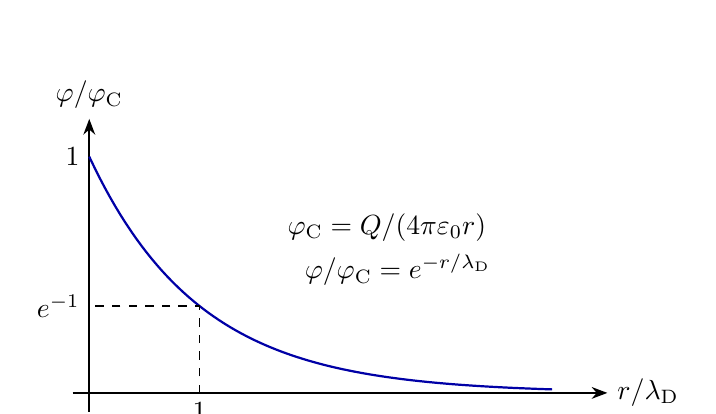
\begin{tikzpicture}[x=1.4cm,y=3cm]
\draw[arr] (-.15,0)--(4.7,0) node[right] {$r/\lambda_{\rm D}$};
\draw[arr] (0,-.08)--(0,1.16) node[above] {$\varphi/\varphi_{\rm C}$};
\draw[blue!65!black,thick,domain=0:4.2,samples=90] plot(\x,{exp(-\x)});
\draw[dashed] (1,0)--(1,.367879)--(0,.367879);
\node[below] at (1,0) {$1$}; \node[left] at (0,1) {$1$};
\node[left] at (0,.367879) {$e^{-1}$};
\node at (2.7,.7) {$\varphi_{\rm C}=Q/(4\pi\varepsilon_0r)$};
\node at (2.8,.52) {$\varphi/\varphi_{\rm C}=e^{-r/\lambda_{\rm D}}$};
\end{tikzpicture}
}
\ifdim\wd\diagrambox>.88\linewidth
\sbox{\diagrambox}{\resizebox{.88\linewidth}{!}{\usebox{\diagrambox}}}
\fi
\ifdim\ht\diagrambox>.29\textheight
\resizebox{!}{.29\textheight}{\usebox{\diagrambox}}
\else\usebox{\diagrambox}\fi
\par\smallskip{\small 图6-2　屏蔽势相对库仑势的比例为 $e^{-r/\lambda_{\rm D}}$；图中长度以德拜长度归一化。\par}
\endgroup\end{minipage}
\end{center}

高频电场中，电子虽然仍受力，但位移幅随 \(\omega^{-2}\)
减小，因此高频极化很弱，介电函数接近真空值。

\subsection{四、解题入口}\label{ux56dbux89e3ux9898ux5165ux53e3-5}

第（1）问由面电荷求场，再写单电子方程。第（2）问先展开电子密度，注意净电荷多一个
\(-e\)，再代入德拜长度定义并用两端边界选取常数。第（3）问从受迫运动求极化，把它与介电函数定义对照，最后判断
\(k^2\) 的正负。

对点电荷的线性化结果，要明确区分线性方程的形式近原点边界，与弱势条件在实际空间中的适用范围。

\subsection{五、解析}\label{ux4e94ux89e3ux6790-5}

（1.1）位移引起的电场。

取单位横向面积，薄层净电荷分别为 \(n_0e\xi\) 与
\(-n_0e\xi\)。每个无限薄层产生的场大小为
\(|\sigma|/(2\varepsilon_0)\)，在两层之间方向相同，相加得

\[
\boxed{\boldsymbol E=\frac{n_0e}{\varepsilon_0}\xi\,\hat{\boldsymbol x}.}
\tag{6.1}
\]

对
\(\xi<0\)，该有向表达式自动反号。薄层的有限厚度使薄层内部电场渐变；式（6.1）是两电荷分离区之间的主体区域电场，符合
\(|\xi|/L\ll1\) 的集体位移近似。

（1.2）恢复运动和等离子体频率。

电子受力为 \(-e\boldsymbol E\)，所以

\[
m_{\rm e}\ddot\xi=-\frac{n_0e^2}{\varepsilon_0}\xi,
\qquad
\ddot\xi+\omega_{\rm p}^2\xi=0.
\]

得到

\[
\boxed{\omega_{\rm p}=\sqrt{\frac{n_0e^2}{m_{\rm e}\varepsilon_0}}.}
\tag{6.2}
\]

若初始位移、速度为 \(\xi_0,u_0\)，解为
\(\xi=\xi_0\cos\omega_{\rm p}t+(u_0/\omega_{\rm p})\sin\omega_{\rm p}t\)。频率与位移幅无关，是线性恢复场的结果。

量纲上，\(e^2/\varepsilon_0\)
的单位为力乘长度平方，再乘数密度并除以质量得到
\(\mathrm{s^{-2}}\)，与角频率平方一致。

（2.1）密度与净电荷。

令 \(z=e\varphi/(k_{\rm B}T)\)，\(|z|\ll1\)，则 \(e^z=1+z+O(z^2)\)，故

\[
\boxed{\delta n(r)=\frac{n_0e}{k_{\rm B}T}\varphi(r).}
\]

正离子数密度保持 \(n_0\)，所以

\[
\rho_q=n_0e-en=-e\delta n,
\qquad
\boxed{\rho_q(r)=-\frac{n_0e^2}{k_{\rm B}T}\varphi(r).}
\tag{6.3}
\]

对
\(Q>0\)，\(\varphi>0\)、\(\delta n>0\)、\(\rho_q<0\)，与电子聚集的物理图像一致。

（2.2）德拜长度。

由题给定义，

\[
\lambda_{\rm D}^2=-\frac{\varepsilon_0\varphi}
{-n_0e^2\varphi/(k_{\rm B}T)}
=\frac{\varepsilon_0k_{\rm B}T}{n_0e^2}.
\]

故

\[
\boxed{\lambda_{\rm D}=\sqrt{\frac{\varepsilon_0k_{\rm B}T}{n_0e^2}}.}
\tag{6.4}
\]

定义中的负号不可遗漏：诱导电荷与电势异号，德拜长度应为正实数。在
\(\varphi=0\) 的点，应把该比值理解为由线性响应系数定义的极限。

（2.3）求球对称屏蔽势。

令 \(\psi=r\varphi\)，则方程转化为

\[
\psi''=\frac{\psi}{\lambda_{\rm D}^2}.
\]

特征根为 \(\pm1/\lambda_{\rm D}\)，所以

\[
\psi=Ae^{-r/\lambda_{\rm D}}+Be^{r/\lambda_{\rm D}}.
\]

要求远处 \(\varphi\to0\)，指数增长项必须消失，即
\(B=0\)。形式近原点匹配要求

\[
\lim_{r\to0}r\varphi=\frac{Q}{4\pi\varepsilon_0},
\]

故 \(A=Q/(4\pi\varepsilon_0)\)。最终

\[
\boxed{\varphi(r)=\frac{Q}{4\pi\varepsilon_0r}e^{-r/\lambda_{\rm D}}.}
\tag{6.5}
\]

当 \(r/\lambda_{\rm D}\ll1\)，指数因子约为
\(1-r/\lambda_{\rm D}\)，势的首项为库仑势。当
\(r/\lambda_{\rm D}\gg1\)，相对库仑势被指数抑制，静电影响主要集中在德拜尺度附近。

必须同时检查弱势条件。对理想点电荷，\(r\to0\) 时 \(|\varphi|\)
发散，因而线性化不可能一直成立到原点。式（6.5）是题给线性方程的点源解，其近原点条件用于确定点源强度；实际弱扰动的使用区间应避开强势核心。

一个保守的尺度判断是
\(r\gg r_*:=|eQ|/(4\pi\varepsilon_0k_{\rm B}T)\)，使未屏蔽库仑势已满足弱势条件。若要同时讨论``近处仍近似库仑势''的实际线性区间，需要
\(r_*\ll r\ll\lambda_{\rm D}\)。若这样的区间不存在，需采用非线性密度响应描述核心，不能只靠线性公式外推。

（2.3续）用总电荷检查屏蔽。

将式（6.5）代入 \(\rho_q=-\varepsilon_0\varphi/\lambda_{\rm D}^2\)，得

\[
\rho_q(r)=-\frac{Q}{4\pi\lambda_{\rm D}^2r}e^{-r/\lambda_{\rm D}}.
\]

在线性点源模型内，诱导总电荷为

\[
Q_{\rm ind}=4\pi\int_0^\infty r^2\rho_q\,dr
=-\frac{Q}{\lambda_{\rm D}^2}\int_0^\infty re^{-r/\lambda_{\rm D}}dr.
\]

令 \(u=r/\lambda_{\rm D}\)，积分等于
\(\lambda_{\rm D}^2\int_0^\infty ue^{-u}du=\lambda_{\rm D}^2\)，故
\(Q_{\rm ind}=-Q\)。

电场为

\[
E_r=-\frac{d\varphi}{dr}
=\frac{Q}{4\pi\varepsilon_0r^2}
\left(1+\frac r{\lambda_{\rm D}}\right)e^{-r/\lambda_{\rm D}}.
\]

其对应的包围净电荷 \(4\pi\varepsilon_0r^2E_r\) 在 \(r\to\infty\)
时趋于零，符合整体屏蔽。

（3.1）电子位移与极化。

在固定位置，把电场局部幅度记为 \(\boldsymbol E_0'\)，电子满足

\[
m_{\rm e}\ddot{\boldsymbol\eta}=-e\boldsymbol E_0'e^{-i\omega t}.
\]

取稳态受迫解 \(\boldsymbol\eta=\boldsymbol\eta_0e^{-i\omega t}\)，代入得

\[
-m_{\rm e}\omega^2\boldsymbol\eta_0=-e\boldsymbol E_0',
\qquad
\boxed{\boldsymbol\eta_0=\frac{e}{m_{\rm e}\omega^2}\boldsymbol E_0'.}
\]

极化为

\[
\boldsymbol P=-n_0e\boldsymbol\eta
=-\frac{n_0e^2}{m_{\rm e}\omega^2}\boldsymbol E.
\]

与定义比较：

\[
\varepsilon_0[\varepsilon(\omega)-1]
=-\frac{n_0e^2}{m_{\rm e}\omega^2},
\]

所以

\[
\boxed{\varepsilon(\omega)=1-\frac{\omega_{\rm p}^2}{\omega^2}.}
\tag{6.6}
\]

电子位移与电场复幅同相，而极化与电场反相，体现了自由电子惯性受迫运动的性质。这里是周期稳态解，任意自由漂移的齐次部分不属于介电响应幅。

（3.2）色散和传播范围。

代入题给色散式：

\[
k^2c^2=\omega^2-\omega_{\rm p}^2,
\qquad
\boxed{\omega^2=\omega_{\rm p}^2+c^2k^2.}
\tag{6.7}
\]

当 \(\omega>\omega_{\rm p}\)，\(k\) 为实数，可形成传播波；当
\(0<\omega<\omega_{\rm p}\)，取向 \(+x\) 衰减的根

\[
k=i\frac{\sqrt{\omega_{\rm p}^2-\omega^2}}c,
\]

场幅随 \(x\) 指数衰减，特征长度为
\(c/\sqrt{\omega_{\rm p}^2-\omega^2}\)。在截止点
\(\omega=\omega_{\rm p}\)，\(k=0\)，不属于具有有限波数的普通传播状态。

本题忽略碰撞，介电函数为实数；低频场的倏逝来自传播条件不满足，不是电子碰撞把能量转化为热。有限厚度介质中的穿透还要由边界条件决定。

\begin{center}
\begin{minipage}{\linewidth}
\centering\begingroup
\sbox{\diagrambox}{\small
\begin{tikzpicture}[x=1.7cm,y=1.2cm]
\draw[arr] (-.15,0)--(3.7,0) node[right] {$ck/\omega_{\rm p}$};
\draw[arr] (0,-.15)--(0,4) node[above] {$\omega/\omega_{\rm p}$};
\draw[dashed,gray] (0,0)--(3.3,3.3) node[right] {真空};
\draw[blue!65!black,thick,domain=0:3.3,samples=90] plot(\x,{sqrt(1+\x*\x)});
\fill (0,1) circle(1.8pt) node[left] {$1$};
\draw[dashed] (1,0)--(1,1.4142)--(0,1.4142);
\node[left] at (0,1.4142) {$\sqrt2$};
\node[below] at (1,0) {$1$};
\node at (2.4,1.1) {$\omega^2=\omega_{\rm p}^2+c^2k^2$};
\end{tikzpicture}
}
\ifdim\wd\diagrambox>.88\linewidth
\sbox{\diagrambox}{\resizebox{.88\linewidth}{!}{\usebox{\diagrambox}}}
\fi
\ifdim\ht\diagrambox>.29\textheight
\resizebox{!}{.29\textheight}{\usebox{\diagrambox}}
\else\usebox{\diagrambox}\fi
\par\smallskip{\small 图6-3　归一化色散曲线：传播支从截止频率开始，群速度小于光速。\par}
\endgroup\end{minipage}
\end{center}

由式（6.7），相速度与群速度分别为

\[
v_{\rm ph}=\frac{\omega}{k}>c,\qquad
v_{\rm g}=\frac{d\omega}{dk}=\frac{c^2k}{\omega}<c.
\]

相速度大于 \(c\) 不表示信号超光速；两者乘积为
\(c^2\)，可作为色散计算的检查。

（3.3）太阳风的频率量级。

按照题给量级：

\[
\omega_{\rm p}\sim
\sqrt{\frac{10^7(10^{-19})^2}{10^{-30}10^{-11}}}
=10^5\,\mathrm{s^{-1}}.
\]

因此普通截止频率

\[
f_{\rm p}=\frac{\omega_{\rm p}}{2\pi}\sim10^4\,\mathrm{Hz}.
\]

可见光 \(f_{\rm vis}\sim10^{14}\,\mathrm{Hz}\)
远大于截止频率，满足传播条件。其介电函数偏离1的量级为

\[
\left|\varepsilon-1\right|
\sim\left(\frac{10^5}{2\pi\times10^{14}}\right)^2
\approx2.5\times10^{-20}.
\]

故在本题无磁场、无碰撞的稀薄等离子体模型中，太阳风对该可见光近似透明。电子仍受到快速交变电场作用，但位移响应幅按
\(\omega^{-2}\) 很小，产生的极化不足以显著改变传播。

（4）从泊松方程重新建立屏蔽方程。

包含原点电荷时，电势满足

\[
\nabla^2\varphi
=-\frac{Q\delta^{(3)}(\boldsymbol r)+\rho_q}{\varepsilon_0}.
\]

用 \(\rho_q=-\varepsilon_0\varphi/\lambda_{\rm D}^2\)，得到

\[
\left(\nabla^2-\frac1{\lambda_{\rm D}^2}\right)\varphi
=-\frac Q{\varepsilon_0}\delta^{(3)}(\boldsymbol r).
\]

在 \(r>0\)，右端为零。球对称情况下，先写

\[
\nabla^2\varphi
=\frac1{r^2}\frac d{dr}\left(r^2\frac{d\varphi}{dr}\right)
=\varphi''+\frac2r\varphi'.
\]

令 \(\psi=r\varphi\)，逐项微分：

\[
\varphi'=\frac{\psi'}r-\frac{\psi}{r^2},\qquad
\varphi''=\frac{\psi''}r-\frac{2\psi'}{r^2}
+\frac{2\psi}{r^3}.
\]

两式组合后交叉项相消，得到
\(\nabla^2\varphi=\psi''/r\)，这才转化成常系数方程
\(\psi''=\psi/\lambda_{\rm D}^2\)。这里先排除原点，是因为点源的奇性不能当成普通函数直接代入局部微分式。

对包围原点的小球使用高斯定理，形式线性点源解的诱导电荷在小球内趋零，故

\[
-\lim_{r\to0}4\pi r^2\varphi'(r)=\frac Q{\varepsilon_0}.
\]

代入 \(\varphi=Ae^{-r/\lambda_{\rm D}}/r\)，左端为 \(4\pi A\)，又得
\(A=Q/(4\pi\varepsilon_0)\)。这由电通量明确了归一化，和先前近原点匹配的形式条件一致。

（5）计算任意半径内的屏蔽电荷。

诱导电荷云在半径 \(r\) 内的总量为

\[
Q_{\rm ind}(<r)
=-\frac Q{\lambda_{\rm D}^2}
\int_0^r s e^{-s/\lambda_{\rm D}}\,ds.
\]

令 \(u=s/\lambda_{\rm D}\)，分部积分给出

\[
\int_0^x u e^{-u}\,du
=\big[-(u+1)e^{-u}\big]_0^x
=1-(1+x)e^{-x}.
\]

于是

\[
Q_{\rm ind}(<r)
=-Q\left[1-\left(1+\frac r{\lambda_{\rm D}}\right)
e^{-r/\lambda_{\rm D}}\right].
\]

点源与诱导云相加，半径 \(r\) 内的净电荷为

\[
Q_{\rm net}(<r)=Q(1+x)e^{-x},\qquad x=\frac r{\lambda_{\rm D}}.
\]

这与电场计算的 \(4\pi\varepsilon_0r^2E_r\) 完全相同。净电荷比例的导数为

\[
\frac d{dx}\big[(1+x)e^{-x}\big]=-xe^{-x}<0\quad(x>0).
\]

所以屏蔽是随半径逐渐积累的过程。\(r=\lambda_{\rm D}\)
时，电势相对库仑势已降为 \(e^{-1}\)，但包围净电荷比例为
\(2/e\)；``屏蔽长度''不能解释为该半径外电荷已经全部抵消。两者分别描述势的比例与高斯通量的比例。

（6）由连续性方程理解纵向集体振荡。

为检查薄层模型的含义，取一维小位移场 \(\xi(x,t)\)。原长 \(dx\)
的电子段变为 \([1+\partial_x\xi]dx\)，粒子数守恒给出

\[
n_0dx=(n_0+\delta n)(1+\partial_x\xi)dx.
\]

丢掉两个小量的乘积，得到
\(\delta n=-n_0\partial_x\xi\)。固定正离子背景下，净电荷为

\[
\rho_q=-e\delta n=n_0e\,\partial_x\xi.
\]

高斯方程 \(\partial_xE=\rho_q/\varepsilon_0\) 因此成为

\[
\partial_x\left(E-\frac{n_0e}{\varepsilon_0}\xi\right)=0.
\]

对于没有额外均匀场、波数非零的纵向扰动，空间常数项取零，故
\(E=n_0e\xi/\varepsilon_0\)。电子动力学随即给出

\[
\ddot\xi=-\frac e{m_{\rm e}}E=-\omega_{\rm p}^2\xi.
\]

这与整体薄层位移具有同一恢复频率。纵向冷电子模式中没有本题横向电磁波的
\(c^2k^2\)
项，因为此处用的是电荷密度与纵向高斯场；不能把两类模式的传播方程混用。

（7）从麦克斯韦方程推出横向色散。

对均匀、非磁性介质中的横向波，\(\boldsymbol k\cdot\boldsymbol E=0\)。采用
\(e^{-i\omega t}\)，法拉第定律和安培定律分别给出

\[
\boldsymbol k\times\boldsymbol E=\omega\boldsymbol B,\qquad
\boldsymbol k\times\boldsymbol B
=-\omega\mu_0\varepsilon_0\varepsilon(\omega)\boldsymbol E.
\]

第一式再左乘 \(\boldsymbol k\times\)，利用三重积

\[
\boldsymbol k\times(\boldsymbol k\times\boldsymbol E)
=\boldsymbol k(\boldsymbol k\cdot\boldsymbol E)-k^2\boldsymbol E
=-k^2\boldsymbol E,
\]

便得到 \(k^2c^2=\varepsilon(\omega)\omega^2\)，其中
\(c^{-2}=\mu_0\varepsilon_0\)。色散式中的真空传播项来自磁场和位移电流，电子响应则通过
\(\varepsilon(\omega)\) 进入。

在 \(\omega>\omega_{\rm p}\) 时，

\[
\omega(k)=\sqrt{\omega_{\rm p}^2+c^2k^2},\qquad
\frac{d\omega}{dk}=\frac{c^2k}{\omega}.
\]

相位前进速率为 \(\omega/k\)，窄带波包的群速为 \(d\omega/dk\)；前者大于
\(c\)、后者小于 \(c\)，两者乘积为 \(c^2\)。截止附近
\(k\to0\)，群速趋零，而相速形式上很大。相速不等于信号前沿速度，不能由它判断超光速传递。

静态屏蔽与动态截止还可用

\[
\lambda_{\rm D}\omega_{\rm p}
=\sqrt{\frac{k_{\rm B}T}{m_{\rm e}}}
\]

联系起来：右端是此处定义的单方向热速度尺度。电子热运动在约一个集体响应时间内跨过的距离，与德拜尺度同量级。这是一种尺度解释，静态屏蔽势和横向倏逝长度仍具有不同方程与边界条件。

\subsection{六、关键洞察}\label{ux516dux5173ux952eux6d1eux5bdf-5}

由式（6.2）与（6.4）可得
\(\lambda_{\rm D}\omega_{\rm p}=\sqrt{k_{\rm B}T/m_{\rm e}}\)。左侧把静态屏蔽尺度和动态响应时间联系起来，右侧是电子的热速度尺度。

点源线性解在原点形式上带有库仑奇点，不等于弱势假设在原点成立。物理上说明实际应用区间，与数学上用点源归一化常数，应分别交代。

\subsection{七、易错点}\label{ux4e03ux6613ux9519ux70b9-5}

\begin{itemize}
\tightlist
\item
  在正电荷电势下写成电子减少，错用玻尔兹曼指数的符号。
\item
  把 \(\delta n\) 当成净电荷密度，漏掉 \(-e\)。
\item
  丢掉德拜长度定义的负号，得到虚长度。
\item
  将指数增长解保留，违反远处边界。
\item
  对 \(e^{-i\omega t}\) 求二阶导数时丢掉负号。
\item
  把 \(\omega_{\rm p}\) 直接当作以赫兹计的截止频率。
\item
  将倏逝等同于吸收，或以相速度大于光速判断信号超光速。
\end{itemize}

\subsection{八、课堂讲解建议}\label{ux516bux8bfeux5802ux8bb2ux89e3ux5efaux8bae-5}

三问都先画电荷与位移方向，再写方程。第（1）问用两薄层各自的场相加，明确为什么不是
\(\sigma/(2\varepsilon_0)\)。第（2）问让学生检查正电势对应的电子势能下降。

第（3）问保持复振幅约定一致，依次写位移、极化、介电函数和色散关系。用图6-3解释实波数、截止和虚波数，最后再作太阳风数量级计算。将``电子无法响应''解释为``响应幅很小''，避免形成电子完全不受力的印象。

\subsection{九、变式训练}\label{ux4e5dux53d8ux5f0fux8badux7ec3-5}

\subsubsection{变式1　密度与温度的缩放}\label{ux53d8ux5f0f1-ux5bc6ux5ea6ux4e0eux6e29ux5ea6ux7684ux7f29ux653e}

把数密度增为原来的4倍，温度增为原来的9倍。求等离子体频率、德拜长度和二者乘积的变化。

\textbf{解答。} 从动力学式得
\(\omega_{\rm p}\propto\sqrt{n_0}\)，故增为2倍。由静态响应
\(\lambda_{\rm D}\propto\sqrt{T/n_0}\)，故增为 \(3/2\) 倍。

两者乘积增为3倍，等于热速度 \(\sqrt{k_{\rm B}T/m_{\rm e}}\)
的变化。可见增加密度同时提高振荡频率和加强静态屏蔽，增加温度则削弱电子聚集而增大屏蔽长度。

\subsubsection{变式2　正离子也参与静态屏蔽}\label{ux53d8ux5f0f2-ux6b63ux79bbux5b50ux4e5fux53c2ux4e0eux9759ux6001ux5c4fux853d}

静态时正离子可移动，其温度为 \(T_i\)，电子温度为
\(T_e\)；未扰动时两者密度均为 \(n_0\)。求总德拜长度。

\textbf{解答。} 电子势能为 \(-e\varphi\)，离子势能为
\(+e\varphi\)，因此一阶响应为

\[
\delta n_e=\frac{n_0e\varphi}{k_{\rm B}T_e},\qquad
\delta n_i=-\frac{n_0e\varphi}{k_{\rm B}T_i}.
\]

净电荷为 \(e\delta n_i-e\delta n_e\)，即

\[
\rho_q=-\frac{n_0e^2\varphi}{k_{\rm B}}
\left(\frac1{T_e}+\frac1{T_i}\right).
\]

故

\[
\frac1{\lambda^2}=\frac{n_0e^2}{\varepsilon_0k_{\rm B}}
\left(\frac1{T_e}+\frac1{T_i}\right).
\]

若两温度相等，总德拜长度为仅电子响应时的
\(1/\sqrt2\)。这是静态平衡问题，不能据此把原题高频电子振荡的质量直接改成离子质量。

\subsubsection{变式3　指定频率的传播与衰减}\label{ux53d8ux5f0f3-ux6307ux5b9aux9891ux7387ux7684ux4f20ux64adux4e0eux8870ux51cf}

分别取 \(\omega=\sqrt2\omega_{\rm p}\) 和
\(\omega=\omega_{\rm p}/2\)。求前者的波数、相速度与群速度，后者的场衰减长度。

\textbf{解答。} 第一种情况 \(c^2k^2=\omega_{\rm p}^2\)，所以

\[
k=\frac{\omega_{\rm p}}c,\quad
v_{\rm ph}=\sqrt2c,\quad v_{\rm g}=\frac c{\sqrt2}.
\]

第二种情况 \(k^2=-3\omega_{\rm p}^2/(4c^2)\)。选择向右衰减的根，场为
\(e^{-\sqrt3\omega_{\rm p}x/(2c)}\)，衰减长度

\[
\ell=\frac{2c}{\sqrt3\omega_{\rm p}}.
\]

两结论分别来自实根与虚根；不能把第二种情况也套进实相速度表达式。

\subsubsection{变式4　加入碰撞阻尼}\label{ux53d8ux5f0f4-ux52a0ux5165ux78b0ux649eux963bux5c3c}

把电子运动改为
\(m_{\rm e}(\ddot{\boldsymbol\eta}+\nu\dot{\boldsymbol\eta})=-e\boldsymbol E\)，\(\nu>0\)。求介电函数和电导率，并检查无碰撞与低频极限。

\textbf{解答。} 用相同的 \(e^{-i\omega t}\) 约定，

\[
(-\omega^2-i\nu\omega)m_{\rm e}\boldsymbol\eta_0=-e\boldsymbol E_0,
\qquad
\boldsymbol\eta_0=\frac{e\boldsymbol E_0}
{m_{\rm e}\omega(\omega+i\nu)}.
\]

故

\[
\varepsilon(\omega)=1-\frac{\omega_{\rm p}^2}{\omega(\omega+i\nu)}.
\]

其虚部为
\(\omega_{\rm p}^2\nu/[\omega(\omega^2+\nu^2)]>0\)，对应该时间约定下的耗散响应。电流密度为
\(\boldsymbol J=-n_0e\dot{\boldsymbol\eta}\)，于是

\[
\sigma(\omega)=\frac{n_0e^2}{m_{\rm e}(\nu-i\omega)}.
\]

\(\nu\to0\) 恢复原介电函数；\(\omega\to0\) 时
\(\sigma\to n_0e^2/(m_{\rm e}\nu)\)，为正的直流电导率。与原题不同，这时传播或倏逝之外还存在真实碰撞吸收。

\clearpage

\section{第 7
题　一维光子晶体的相干反射与缺级}\label{ux7b2c-7-ux9898-ux4e00ux7ef4ux5149ux5b50ux6676ux4f53ux7684ux76f8ux5e72ux53cdux5c04ux4e0eux7f3aux7ea7}

折射率呈周期空间分布的材料称为光子晶体。假设所有介质均为线性、非磁性，折射率为实数。真空光速为
\(c\)，单色电场写为 \(\operatorname{Re}[E(x)e^{-i\omega t}]\)，真空波数
\(k=\omega/c\)。

（1）单界面位于 \(x=0\)，左侧折射率 \(n_1\)，右侧
\(n_2\)。光从左侧正入射，界面处 \(E\) 和 \(dE/dx\)
连续。定义电场幅反射系数 \(r=E_r/E_i\)、透射系数 \(t=E_t/E_i\)，求
\(r,t\)。

（2）晶体第一界面位于 \(x=0\)，每个周期先是折射率 \(n_2\)、厚度 \(d_2\)
的层，再是折射率 \(n_1\)、厚度 \(d_1\) 的层，共 \(N\)
个完整周期。晶体外两侧折射率均为 \(n_1\)。光从左侧沿 \(+x\)
正入射。\(N\gg1\) 时，反射幅的模随频率出现主极大。

（2.1）\(\delta n=n_1-n_2\) 为小量。求总反射系数 \(r_{\rm tot}\)
的模，保留对折射率差的一阶项；求第 \(m\) 个可能主极大的角频率
\(\omega_m\)，\(m=1,2,\ldots\)；求主极大不能实现的缺级条件。若
\(\omega_m\) 缺级，令 \(\omega=\omega_m+\epsilon\)，求模的首个非零近似。

（2.2）定义等效波矢大小 \(\bar k=\bar n k\)，其中

\[
\bar n=\frac{n_1d_1+n_2d_2}{d_1+d_2}.
\]

在 \(\omega_m\) 处，求从向前等效波矢 \(\bar k\) 到向后 \(-\bar k\)
的变化与空间周期 \(d_1+d_2\) 的关系，说明物理含义。本题45分。

\begin{center}
\begin{minipage}{\linewidth}
\centering\begingroup
\sbox{\diagrambox}{\small
\begin{tikzpicture}
\fill[gray!10] (-2,1.9) rectangle (0,4);
\fill[blue!12] (0,1.9) rectangle (2,4);
\draw[thick] (0,1.9)--(0,4);
\draw[arr] (-1.8,3.5)--(-.25,3.5) node[midway,above] {$E_i$};
\draw[arr] (-.25,2.7)--(-1.8,2.7) node[midway,above] {$E_r$};
\draw[arr] (.2,3.3)--(1.8,3.3) node[midway,above] {$E_t$};
\node at (-1,2.2) {$n_1$}; \node at (1,2.2) {$n_2$};
\node at (0,1.5) {$x=0$};
\fill[gray!10] (-2,-1.3) rectangle (0,.6);
\fill[gray!10] (6.4,-1.3) rectangle (7.5,.6);
\node at (-1,-.8) {$n_1$}; \node at (7,-.6) {$n_1$};
\foreach \p in {0,1,2,3} {
 \fill[blue!16] (1.6*\p,-1.3) rectangle (1.6*\p+.65,.6);
 \fill[gray!10] (1.6*\p+.65,-1.3) rectangle (1.6*\p+1.6,.6);
 \draw (1.6*\p,-1.3)--(1.6*\p,.6);
 \node at (1.6*\p+.325,-.6) {$n_2$};
 \node at (1.6*\p+1.12,-.6) {$n_1$};}
\draw[arr] (-2,-.3)--(-.2,-.3) node[midway,above] {入射};
\draw[arr] (-2,-1.3)--(8,-1.3) node[right] {$x$};
\draw[<->] (0,.9)--(.65,.9) node[midway,above] {$d_2$};
\draw[<->] (.65,.9)--(1.6,.9) node[midway,above] {$d_1$};
\draw[<->] (0,-1.9)--(6.4,-1.9) node[midway,below] {$N$ 个完整周期（示意）};
\node[below] at (0,-1.3) {$0$};
\end{tikzpicture}
}
\ifdim\wd\diagrambox>.88\linewidth
\sbox{\diagrambox}{\resizebox{.88\linewidth}{!}{\usebox{\diagrambox}}}
\fi
\ifdim\ht\diagrambox>.29\textheight
\resizebox{!}{.29\textheight}{\usebox{\diagrambox}}
\else\usebox{\diagrambox}\fi
\par\smallskip{\small 图7-1　单界面的入射、反射和透射，以及晶体的层序与完整周期。\par}
\endgroup\end{minipage}
\end{center}

\subsection{一、题型定位}\label{ux4e00ux9898ux578bux5b9aux4f4d-6}

本题从界面反射推出多界面相干叠加，数学形式与多缝干涉相似。每周期内两个界面的反射符号相反，构成单周期包络；各周期之间的反射相位差相同，构成几何级数。

折射率差小允许先计算单次反射路径，但大层数会增强相干反射。靠近主极大时，还须检查总幅是否仍在弱反射范围内。

\subsection{二、知识点}\label{ux4e8cux77e5ux8bc6ux70b9-6}

\begin{itemize}
\tightlist
\item
  \(e^{+inkx}\) 与 \(e^{-inkx}\) 分别代表向右、向左传播的空间幅。
\item
  边界导数条件包含反射波的负波矢。
\item
  电场幅系数可为负，负号表示相位反转；它不是能量反射率。
\item
  光程决定传播相位，反射路径需要计算往返光程。
\item
  相同相位差的 \(N\) 项相干和是几何级数。
\item
  缺级要求周期间同相增强与周期内相消同时发生。
\item
  反向散射的波矢差与周期结构的倒格矢相匹配。
\end{itemize}

\subsection{三、物理图像}\label{ux4e09ux7269ux7406ux56feux50cf-6}

记空间周期 \(a=d_1+d_2\)，单程周期光程 \(S=n_1d_1+n_2d_2\)。第 \(p\)
个周期，\(p=0,\ldots,N-1\)，有两个反射位置：\(x=pa\) 的 \(n_1\to n_2\)
界面，以及 \(x=pa+d_2\) 的 \(n_2\to n_1\) 界面。

第一类界面的反射系数是 \(r\)，第二类是 \(-r\)。两束反射在回到 \(x=0\)
时还相差相位 \(2kn_2d_2\)。不同周期之间相差 \(2kS\)。

\begin{center}
\begin{minipage}{\linewidth}
\centering\begingroup
\sbox{\diagrambox}{\small
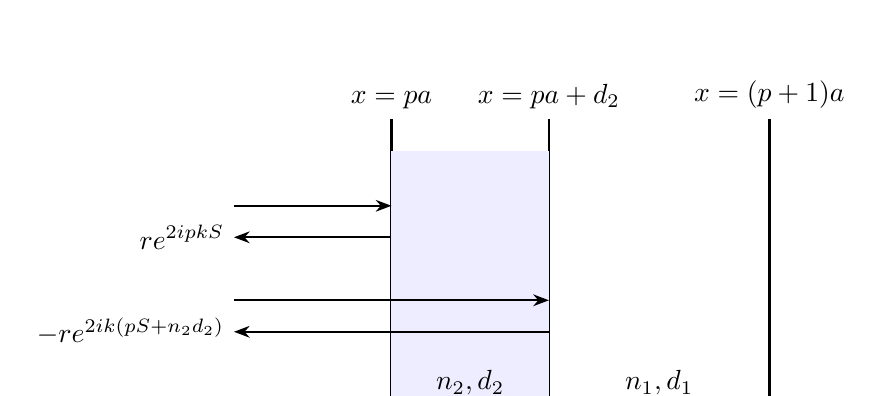
\begin{tikzpicture}
\draw[thick] (0,-1.5)--(0,2.2) node[above] {$x=pa$};
\draw[thick] (2,-1.5)--(2,2.2) node[above] {$x=pa+d_2$};
\draw[thick] (4.8,-1.5)--(4.8,2.2) node[above] {$x=(p+1)a$};
\fill[blue!7] (0,-1.5) rectangle (2,1.8);
\node at (1,-1.15) {$n_2,d_2$};
\node at (3.4,-1.15) {$n_1,d_1$};
\draw[arr] (-2,1.1)--(0,1.1);
\draw[arr] (0,.7)--(-2,.7);
\draw[arr] (-2,-.1)--(2,-.1);
\draw[arr] (2,-.5)--(-2,-.5);
\node[left] at (-2,.7) {$r e^{2ipkS}$};
\node[left] at (-2,-.5) {$-r e^{2ik(pS+n_2d_2)}$};
\end{tikzpicture}
}
\ifdim\wd\diagrambox>.88\linewidth
\sbox{\diagrambox}{\resizebox{.88\linewidth}{!}{\usebox{\diagrambox}}}
\fi
\ifdim\ht\diagrambox>.29\textheight
\resizebox{!}{.29\textheight}{\usebox{\diagrambox}}
\else\usebox{\diagrambox}\fi
\par\smallskip{\small 图7-2　每周期的两条单次反射路径；往返相位分别为 $2pkS$ 与 $2pkS+2kn_2d_2$。\par}
\endgroup\end{minipage}
\end{center}

因此增强有两层条件：各周期反射要同相，周期内的一对反射不能互相抵消。前者给出布拉格中心，后者给出包络和缺级。

\subsection{四、解题入口}\label{ux56dbux89e3ux9898ux5165ux53e3-6}

先写左右电场并用两个边界条件求
\(r,t\)。对晶体，保留每个界面一次反射的贡献，把 \(2N\)
项先按周期成对，再求几何级数。

求主极大时不能把分母为零当成发散：分子也趋零，其比值极限为
\(N\)。求缺级附近时要保留周期光程 \(S\)，最后在 \(\epsilon\to0\)
的极限中消去它。

\subsection{五、解析}\label{ux4e94ux89e3ux6790-6}

（1）单界面幅系数。

令入射幅为1。左侧与右侧分别写为

\[
E_-(x)=e^{in_1kx}+r e^{-in_1kx},\qquad
E_+(x)=t e^{in_2kx}.
\]

在 \(x=0\)，电场连续给出 \(1+r=t\)，导数连续给出

\[
in_1k(1-r)=in_2kt.
\]

消去 \(t\)：

\[
n_1-n_1r=n_2+n_2r,
\]

所以

\[
\boxed{r=\frac{n_1-n_2}{n_1+n_2},\qquad
t=\frac{2n_1}{n_1+n_2}.}
\tag{7.1}
\]

当 \(n_2>n_1\)，\(r<0\)，反射场有 \(\pi\)
相位变化。透射幅可能大于1，但不表示透射能量超过入射能量。非磁性实折射率介质中，

\[
R=|r|^2,\qquad T=\frac{n_2}{n_1}|t|^2,
\]

代入得到 \(R+T=1\)，是单界面结果的守恒检查。

（2.1）说明一阶路径近似。

反向界面的系数为 \(r_{21}=-r\)。一对正反界面的透射幅乘积为

\[
t_{12}t_{21}=\frac{4n_1n_2}{(n_1+n_2)^2}=1-r^2.
\]

因此在固定层数的一阶反射计算中，往返透射系数乘积可取1。多次反射路径含更高次的
\(r\)，不属于本题要求的一阶项；只留下 \(2N\) 条单次反射路径。

一阶叠加在布拉格附近可能增至
\(O(Nr)\)，要把它作为准确弱反射近似使用，充分的保守条件是
\(N|r|\ll1\)。若这个条件不满足，仍可利用一阶式识别相位匹配中心，但强反射率和带隙须由完整多次反射模型计算。

（2.1续）写每周期的反射幅。

到第一个界面的往返光程为 \(2pS\)，到第二个界面的往返光程为
\(2pS+2n_2d_2\)。该周期贡献为

\[
r_p=r e^{2ipkS}-r e^{2ik(pS+n_2d_2)}
=r(1-e^{2ikn_2d_2})e^{2ipkS}.
\]

于是

\[
r_{\rm tot}=r(1-e^{2ikn_2d_2})
\sum_{p=0}^{N-1}e^{2ipkS}.
\tag{7.2}
\]

几何级数公式给出

\[
r_{\rm tot}=r(1-e^{2ikn_2d_2})
\frac{1-e^{2iNkS}}{1-e^{2ikS}}.
\]

当 \(e^{2ikS}=1\) 时，应直接用有限和的值
\(N\)，而不是把这个商理解成无穷大。

由 \(|1-e^{2iu}|=2|\sin u|\) 得

\[
\boxed{|r_{\rm tot}|=
\frac{2|\delta n|}{n_1+n_2}|\sin(kn_2d_2)|
\left|\frac{\sin(NkS)}{\sin(kS)}\right|.}
\tag{7.3}
\]

这里保留了相位中的实际光程。其含折射率差的高阶影响不改变式（7.3）所代表的单次反射一阶结构。

（2.1续）可能主极大的频率。

各周期反射同相要求 \(2k_mS=2m\pi\)，即

\[
\boxed{\omega_m=\frac{m\pi c}{S},\qquad m=1,2,\ldots.}
\tag{7.4}
\]

在该布拉格中心，周期和为 \(N\)。若周期内包络不为零，则

\[
|r_{\rm tot}(\omega_m)|
=2N|r|\left|\sin\left(\frac{m\pi n_2d_2}{S}\right)\right|.
\]

对于 \(N\gg1\)，主峰集中在式（7.4）附近。有限 \(N\)
时若包络具有非零斜率，总函数的实际极大点会相对布拉格中心发生小移位；式（7.4）是本题采用的大
\(N\) 主极大位置近似。包络非零且变化平缓时，这个移位为 \(O(N^{-2})\)
的频率尺度修正。

（2.1续）缺级。

当 \(k_mn_2d_2=l\pi\) 时，同一周期内两个反射贡献相消。于是缺级条件是

\[
\boxed{\frac{m n_2d_2}{S}=l,\qquad
l\in\mathbb Z,\quad 1\le l<m.}
\tag{7.5}
\]

正整数范围来自
\(0<n_2d_2/S<1\)。缺级不表示该频率周围完全没有反射；它表示本应增强的布拉格中心恰好被周期内相消压成零。

令 \(q=n_2d_2/S\)。若 \(q=p/s\) 为最简有理数，则缺级阶数是
\(m=s,2s,\ldots\)；若 \(q\)
为无理数，不存在满足式（7.5）的整数阶精确缺级。

（2.1续）缺级附近首个非零项。

取 \(\omega=\omega_m+\epsilon\)，\(k=k_m+\epsilon/c\)。在缺级中心，

\[
|\sin(kn_2d_2)|=
\left|\sin\left(l\pi+\frac{\epsilon n_2d_2}{c}\right)\right|
\simeq\frac{n_2d_2}{c}|\epsilon|.
\]

周期和的比值则为

\[
\left|\frac{\sin(NkS)}{\sin(kS)}\right|
=\left|\frac{\sin(N\epsilon S/c)}{\sin(\epsilon S/c)}\right|
\longrightarrow N.
\]

因此

\[
\boxed{|r_{\rm tot}(\omega_m+\epsilon)|
\simeq\frac{2N|\delta n|n_2d_2}{c(n_1+n_2)}|\epsilon|.}
\tag{7.6}
\]

此式要求
\(|\epsilon|NS/c\ll1\)，使观察点处于缺级中心足够近的区域。模必须非负，所以保留
\(|\epsilon|\)；若写反射强度，则首项与 \(\epsilon^2\) 成正比。

\begin{center}
\begin{minipage}{\linewidth}
\centering\begingroup
\sbox{\diagrambox}{\small
\begin{tikzpicture}[x=.68cm,y=.9cm]
\foreach \p in {0,1,2,3,4} \draw[arr] (\p*1.2,1)--(\p*1.2+1,1);
\node at (3,1.75) {$2kS=2m\pi$：各周期同相};
\draw[arr] (0,-1.4)--(1.5,-1.4);
\draw[arr] (3,-1.4)--(1.5,-1.4);
\node at (5,-1.4) {$r-r e^{2il\pi}=0$};
\node at (3,-2.1) {缺级：同周期内相消};
\begin{scope}[shift={(12,-1)},x=1cm,y=1cm]
\draw[arr] (-1.5,0)--(1.6,0) node[right] {$\epsilon$};
\draw[arr] (0,-.2)--(0,2) node[above] {$|r_{\rm tot}|$};
\draw[thick,blue!65!black] (-1.2,1.4)--(0,0)--(1.2,1.4);
\node[below] at (0,0) {$0$};
\end{scope}
\end{tikzpicture}
}
\ifdim\wd\diagrambox>.88\linewidth
\sbox{\diagrambox}{\resizebox{.88\linewidth}{!}{\usebox{\diagrambox}}}
\fi
\ifdim\ht\diagrambox>.29\textheight
\resizebox{!}{.29\textheight}{\usebox{\diagrambox}}
\else\usebox{\diagrambox}\fi
\par\smallskip{\small 图7-3　周期间相干增强与周期内缺级的区别；缺级中心附近的幅模呈线性尖谷。\par}
\endgroup\end{minipage}
\end{center}

（2.2）波矢变化和空间周期。

按题给定义，\(\bar k=(S/a)k\)。在式（7.4）的频率，

\[
\bar k_m=\frac{S}{a}\frac{m\pi}{S}=\frac{m\pi}{a}.
\]

向前与向后波矢之差的大小为

\[
\boxed{2\bar k_m=\frac{2m\pi}{a}.}
\tag{7.7}
\]

从入射波矢 \(+\bar k_m\) 到反射波矢 \(-\bar k_m\) 的有向变化为
\(-2\bar k_m\)；其大小等于第 \(m\) 个倒格矢 \(2m\pi/a\)。

相位解释最直接：每增加一个完整周期的往返路径，相位增加
\(2\bar k_ma=2m\pi\)，故各周期反射同相。也可理解为周期结构允许与其倒格矢匹配的反向散射。此处的
\(\bar k\)
是题目定义的等效传播量，完整强对比光子晶体的布洛赫波矢还需要另行求解。

（补充核对）缺级与守恒的相容性。

单次反射式可能给出
\(2N|r|>1\)，而无损结构的实际反射幅不应超过1。这不说明能量不守恒，而说明在该参数下更高次路径必须保留。缺级中心相消属于一阶反射结论；在严格一维无损层状模型的特定整周期相位条件下，还可用传输矩阵进一步检查其精确性。

（3）逐项求几何级数的幅与相位。

令 \(z=e^{2ikS}\)。有限和 \(G_N=1+z+\cdots+z^{N-1}\) 满足

\[
(1-z)G_N=1-z^N.
\]

利用 \(1-e^{2iu}=-2ie^{iu}\sin u\)，不仅能求模，还能保留共同相位：

\[
G_N=e^{i(N-1)kS}\frac{\sin(NkS)}{\sin(kS)}.
\]

单周期因子为 \(1-e^{2ikn_2d_2}=-2ie^{ikn_2d_2}\sin(kn_2d_2)\)，因此

\[
r_{\rm tot}
=-2ir\,e^{i[(N-1)kS+kn_2d_2]}
\sin(kn_2d_2)\frac{\sin(NkS)}{\sin(kS)}.
\]

共同复相位不改变幅模，却影响反射场与别的参考场的干涉。三角函数比可为负；把它整体取绝对值只适用于求模，不能在复振幅求和过程中提前抹去符号。

在布拉格中心 \(kS=m\pi\)，几何级数原式每项均为1，故
\(G_N=N\)。三角函数比的极限本身可能带有
\((-1)^{(N-1)m}\)，共同相位又提供相同符号，两者相乘才回到
\(N\)。这说明求模时看不到的相位仍需在复幅中一致处理。

（4）定量说明有限层数主峰的移位。

设该级次不缺级，记

\[
q=\frac{n_2d_2}{S},\qquad y=kS-m\pi,\qquad a_m=m\pi q.
\]

中心附近的幅模除去常数后为 \(|\sin(a_m+qy)|\,|\sin(Ny)/\sin y|\)。当
\(|Ny|\ll1\)，

\[
\frac{\sin(Ny)}{\sin y}
=N\left[1-\frac{N^2-1}{6}y^2+O(N^4y^4)\right].
\]

要找极大，可对幅的对数求导。包络不为零且变化平缓时，

\[
\frac d{dy}\log|r_{\rm tot}|
=q\cot a_m
-\left[q^2\csc^2a_m+\frac{N^2-1}{3}\right]y
+O(y^2)+O(N^4y^3).
\]

因此峰的领先阶移位为

\[
y_{\rm peak}\simeq
\frac{q\cot a_m}
{q^2\csc^2a_m+(N^2-1)/3},\qquad
\delta\omega_{\rm peak}=\frac cS y_{\rm peak}.
\]

远离缺级、\(q\cot a_m\)
为通常有限量时，\(y_{\rm peak}=O(N^{-2})\)；主峰宽度却为
\(O(N^{-1})\)，所以大 \(N\) 下以布拉格中心代表主极大位置是合理近似。若
\(\sin a_m\)
很小，对数展开不再平缓，应回到原函数求峰，不能将这一公式用于缺级中心。

（5）建立完整层传播矩阵。

单次路径法给出弱反射答案。作为完整替代模型，取场状态

\[
\boldsymbol u(x)=
\begin{pmatrix}E(x)\\E'(x)/(ik)\end{pmatrix}.
\]

题给的两个连续条件正好要求这个状态在界面连续。均匀层内
\(E''+n^2k^2E=0\)，由入口的场和导数决定出口：

\[
\boldsymbol u(x+d)=M(n,d)\boldsymbol u(x),
\]

\[
M(n,d)=
\begin{pmatrix}
\cos\delta&i\sin\delta/n\\
in\sin\delta&\cos\delta
\end{pmatrix},\qquad \delta=nkd.
\]

矩阵由正、反传播两束波共同解出的，因此已经包含完整多次反射，而非只选择单次路径。其行列式为
\(\cos^2\delta+\sin^2\delta=1\)。

本题每周期先通过 \(n_2\) 层，再通过 \(n_1\) 层，列向量右侧先作用，故

\[
M_{\rm cell}=M(n_1,d_1)M(n_2,d_2),\qquad
P=M_{\rm cell}^{\,N}.
\]

不能颠倒乘法顺序后仍保留同一入口定义。晶体两侧折射率均为
\(n_1\)，将入口入射幅设为1，则

\[
\boldsymbol u_{\rm left}
=\begin{pmatrix}1+r_N\\n_1(1-r_N)\end{pmatrix},\qquad
\boldsymbol u_{\rm right}
=\begin{pmatrix}t_N\\n_1t_N\end{pmatrix}.
\]

令

\[
\begin{aligned}
a&=P_{11}+n_1P_{12},& b&=P_{11}-n_1P_{12},\\
c_1&=P_{21}+n_1P_{22},& d&=P_{21}-n_1P_{22},
\end{aligned}
\]

两个出口条件成为 \(t_N=a+br_N\)、\(n_1t_N=c_1+dr_N\)。消去透射幅，得到

\[
r_N=\frac{c_1-n_1a}{n_1b-d},\qquad
t_N=a+br_N.
\]

这样可以在任意层数下计算反射，并检查同侧介质中的
\(|r_N|^2+|t_N|^2=1\)。小折射率差、固定 \(N\)
时展开矩阵结果，必须恢复前面的单次路径式；相干增强导致 \(N|r|\)
不小时，应使用完整矩阵结果。

（6）矩阵如何解释缺级与周期结构。

直接乘开一个周期的矩阵，半迹为

\[
\frac{\operatorname{tr}M_{\rm cell}}2
=\cos\delta_1\cos\delta_2
-\frac12\left(\frac{n_1}{n_2}+\frac{n_2}{n_1}\right)
\sin\delta_1\sin\delta_2.
\]

因为行列式为1，两个本征值互为倒数。若写作 \(e^{\pm iKa}\)，有
\(\cos(Ka)=\operatorname{tr}M_{\rm cell}/2\)。这是完整周期模型中的布洛赫波矢
\(K\)，与题目人为定义的平均波矢 \(\bar k\)
有不同定义；弱对比下两者在传播相位的领先阶可相联系。

在缺级中心，\(\delta_2=l\pi\)，且
\(\delta_1=(m-l)\pi\)。于是每一层的矩阵都是带符号的单位矩阵：

\[
M_2=(-1)^lI,\qquad M_1=(-1)^{m-l}I,
\]

\[
M_{\rm cell}=(-1)^mI,\qquad P=(-1)^{mN}I.
\]

代入入口、出口条件，严格得到
\(r_N=0\)、\(t_N=(-1)^{mN}\)。因此对本题无损、两侧同介质、完整周期的层状模型，满足两个整半波光学厚度条件的缺级中心也具有精确零反射。其附近的线性尖谷则由频率微小偏离破坏这一整相位条件产生。

\subsection{六、关键洞察}\label{ux516dux5173ux952eux6d1eux5bdf-6}

反射的频谱由``单周期的一对界面''与``多个周期的排列''共同决定。只看周期排列能得到主峰中心，却无法解释缺级；只看一对界面则无法解释峰随层数变窄。

层数大和折射率差小是两个独立条件。若先固定小折射率差再让层数无限大，近峰的单次反射近似会失效。需要根据所求量区分相位匹配的预测与反射率的定量计算。

\subsection{七、易错点}\label{ux4e03ux6613ux9519ux70b9-6}

\begin{itemize}
\tightlist
\item
  忘记反射波导数中的负号，求错单界面系数。
\item
  将两类界面反射都写成 \(+r\)，丢掉周期内相消。
\item
  用单程相位代替往返相位，主峰频率相差一倍。
\item
  在 \(x=Na\) 处多算一个不存在的折射率界面。
\item
  分母为零时判断反射发散，没有求有限和的极限。
\item
  缺级展开中遗漏光程 \(S\)，中间式出现量纲不一致。
\item
  幅模写成与有向 \(\epsilon\) 成正比，而非与 \(|\epsilon|\) 成正比。
\item
  把弱反射幅平方式外推到大于1的反射率。
\end{itemize}

\subsection{八、课堂讲解建议}\label{ux516bux8bfeux5802ux8bb2ux89e3ux5efaux8bae-6}

先完成一个界面的边界条件，再只画一个周期，标出反射符号与往返相位。确认周期内贡献后，才将它复制为
\(N\) 项几何级数。

求主极大时先令各项同相，直接得到和为
\(N\)；这样可以避免把三角函数比误看成发散。缺级部分选用等光学厚度的例子，展示奇数阶增强、偶数阶消失。最后讨论增加层数引起的峰变窄与近似失效。

\subsection{九、变式训练}\label{ux4e5dux53d8ux5f0fux8badux7ec3-6}

\subsubsection{变式1　等光学厚度双层}\label{ux53d8ux5f0f1-ux7b49ux5149ux5b66ux539aux5ea6ux53ccux5c42}

令 \(n_1d_1=n_2d_2\)，求哪些布拉格级次缺级，并求不缺级中心的一阶反射幅。

\textbf{解答。} 此时 \(q=n_2d_2/S=1/2\)。在第 \(m\) 阶中心，包络为
\(|\sin(m\pi/2)|\)。偶数 \(m\) 时为零，故缺级；奇数 \(m\) 时为1，故

\[
|r_{\rm tot}(\omega_m)|=2N|r|.
\]

第一中心频率为 \(\omega_1=\pi c/S\)，对应各层单程相位
\(\pi/2\)，即常见的四分之一波光学厚度条件。幅随 \(N\) 线性增加仅限
\(N|r|\ll1\)；更厚结构须计入多次反射。

\subsubsection{变式2　指定缺级阶数}\label{ux53d8ux5f0f2-ux6307ux5b9aux7f3aux7ea7ux9636ux6570}

设 \(n_2d_2/S=2/5\)，求首个缺级、物理厚度比及前四阶中心幅。

\textbf{解答。} 缺级要求 \(2m/5\) 为整数，最小正阶为
\(m=5\)，其后为10、15等。由 \(5n_2d_2=2(n_1d_1+n_2d_2)\) 得

\[
\frac{d_2}{d_1}=\frac{2n_1}{3n_2}.
\]

前四阶幅为 \(2N|r||\sin(2m\pi/5)|\)，即

\[
2N|r|\{\sin(2\pi/5),\ \sin(\pi/5),\
\sin(\pi/5),\ \sin(2\pi/5)\}.
\]

第5阶的周期间反射仍同相，却被周期内相消压为零。这里缺级由光学厚度比决定，不能只按物理厚度
\(d_2/a\) 判断。

\subsubsection{变式3　允许主峰的零点宽度}\label{ux53d8ux5f0f3-ux5141ux8bb8ux4e3bux5cf0ux7684ux96f6ux70b9ux5bbdux5ea6}

在包络非零且主峰附近变化缓慢的条件下，求第 \(m\)
阶中心两侧最近的干涉零点与零点间宽度。

\textbf{解答。} 写 \(\omega=\omega_m+\epsilon\)，周期因子为
\(|\sin(N\epsilon S/c)/\sin(\epsilon S/c)|\)。最近非零根来自
\(N\epsilon S/c=\pm\pi\)，故

\[
\epsilon_\pm=\pm\frac{\pi c}{NS}.
\]

两零点间频率宽度为

\[
\Delta\omega_{\rm zero}=\frac{2\pi c}{NS}.
\]

它随层数反比减小。若换成普通频率，宽度为
\(c/(NS)\)。这不是半高宽；缺级中心附近也不能直接沿用允许主峰的包络常量近似。

\par\noindent\begin{minipage}{\linewidth}
\setlength{\parindent}{2em}\setlength{\parskip}{.35em}
\subsubsection{变式4　一层薄膜的精确多次反射}\label{ux53d8ux5f0f4-ux4e00ux5c42ux8584ux819cux7684ux7cbeux786eux591aux6b21ux53cdux5c04}

仅取一层折射率 \(n_2\)、厚度 \(d_2\) 的薄膜，两侧均为 \(n_1\)。令
\(\delta=n_2kd_2\)，求精确反射幅，比较一阶式。

\textbf{解答。} 第一界面直接反射为
\(r\)。进入薄膜、在右界面反射并返回左侧的第一项为
\(-r(1-r^2)e^{2i\delta}\)。每增加一次薄膜内部往返，又乘
\(r^2e^{2i\delta}\)，因为从膜内看两界面的反射系数均为 \(-r\)。

几何级数相加：

\[
r_{\rm slab}=r-\frac{r(1-r^2)e^{2i\delta}}
{1-r^2e^{2i\delta}}
=\frac{r(1-e^{2i\delta})}{1-r^2e^{2i\delta}}.
\]

透射幅为

\[
t_{\rm slab}=\frac{(1-r^2)e^{i\delta}}
{1-r^2e^{2i\delta}}.
\]

同折射率入射、出射介质使功率透射率等于
\(|t_{\rm slab}|^2\)。分母模平方为 \((1-r^2)^2+4r^2\sin^2\delta\)，从而

\[
|r_{\rm slab}|^2+|t_{\rm slab}|^2
=\frac{4r^2\sin^2\delta+(1-r^2)^2}
{(1-r^2)^2+4r^2\sin^2\delta}=1.
\]

当 \(|r|\ll1\)，精确式变为 \(r(1-e^{2i\delta})+O(r^3)\)，恰好恢复本题
\(N=1\) 的单次反射贡献；当 \(\delta=l\pi\)，精确反射也为零。

\end{minipage}\par

\end{document}
